\documentclass[11pt,a4paper]{article}
\usepackage[T1]{fontenc}
\usepackage[utf8]{inputenc}
\usepackage{lmodern}
\usepackage[margin=27mm]{geometry}
\usepackage{amsmath,amssymb,amsthm,mathtools}
\usepackage{microtype,booktabs}
\usepackage{graphicx}
\usepackage[colorlinks=true,linkcolor=blue,citecolor=blue,urlcolor=blue]{hyperref}
\numberwithin{equation}{section}
\newtheorem{theorem}{Theorem}[section]
\newtheorem{lemma}[theorem]{Lemma}
\newtheorem{proposition}[theorem]{Proposition}
\newtheorem{corollary}[theorem]{Corollary}
\theoremstyle{definition}
\newtheorem{definition}[theorem]{Definition}
\theoremstyle{remark}
\newtheorem{remark}[theorem]{Remark}
\newcommand{\dd}{\mathop{}\!\mathrm d}
\newcommand{\cH}{\mathcal H}
\newcommand{\cF}{\mathcal F}
\newcommand{\cS}{\mathcal S}
\newcommand{\cE}{\mathcal E}
\newcommand{\cM}{\mathcal M}
\newcommand{\cD}{\mathcal D}
\newcommand{\Cc}{C_c^\infty}
\newcommand{\FP}{\mathrm{FP}}
\newcommand{\GA}{\mathrm{GA}}
\newcommand{\gen}{\mathrm{gen}}
\newcommand{\spec}{\mathrm{spec}}
\newcommand{\Sym}{\operatorname{Sym}}
\newcommand{\supp}{\operatorname{supp}}
\newcommand{\sech}{\operatorname{sech}}
\newcommand{\norm}[1]{\left\lVert#1\right\rVert}
\newcommand{\ip}[2]{\left\langle#1,#2\right\rangle}
\newcommand{\rhoP}{\rho_{\mathrm{Pl}}}
\newcommand{\KP}{K_{\mathrm P}}
\newcommand{\one}{\mathbf 1}
\DeclareMathOperator*{\esssup}{ess\,sup}
\title{Physical state spaces and Gaussian observables\\
for quantum observers in de Sitter space}
\author{Alan Day \and Chengheng\thanks{AI research assistant (OpenAI).}}
\date{Working research draft --- 30 October 2026}
\begin{document}
\maketitle
\begin{abstract}
We study two quantum observers and free principal-series matter on
two-dimensional de Sitter space in the strict $G_{\!N}\to0$ limit. We specify a
weak positive-frequency condition directly on finite gauge-fixed position
states and identify the resulting maximal space with the closure of actual
group-averaged observer wave packets. The analytic step is a complete
position-test core controlled by a fractional radial moment: a low-energy
spectral cutoff converges in the orbit norm although a first-moment estimate
would not suffice. The identification retains both continuous
Clebsch--Gordan channels and all internal discrete paths. With explicit
Gaussian proper-time smearing and repeated observer mass projections,
bounded equivariant creation blocks descend through a common group cutoff.
Their symmetric field is essentially self-adjoint on the full finite-particle
domain. On explicit seed tests, the creation block also admits an
absolutely convergent position pairing for every physical input; auxiliary
position and group cutoffs can be removed in that pairing. For annihilation,
finite emitted-mode position integrals converge in physical dual norm at
each seed test; on physical seed inputs, a positive Fej\'er regulator also
gives an absolutely convergent uncut position formula.
We also record the connection to ordered four-point functions of two
independent matter species. These are statements about a specified
weak-frequency realization and regulated observables, not a construction of
a finite-$G_N$ holographic dual.
\end{abstract}

\section{Introduction and scope}
The two-observer model of Kolchmeyer and Liu~\cite{KL} makes observer recoil
and relational correlators accessible while the background remains fixed.
An important distinction in this model is between a kinematical Hilbert
space, non-normalizable invariant coefficients, and a physical Hilbert
space defined by a gauge-fixed position norm. Statements about one of these
spaces need not extend to the others by ordinary Hilbert-space density.
In particular, evaluation on a continuous spectral diagonal is not a bounded
operation on the kinematical tensor product.

We work with de Sitter radius $L=1$, the proper group $G=SO^+(2,1)$, and
real principal-series matter parameters $\nu>0$. The physical observer mass
associated with a representation label $s$ is
\begin{equation}
 m(s)=\sqrt{s^2+\tfrac14}.
\end{equation}
Unless a zero-threshold extension is explicitly stated, each actual observer
has a fixed lower label $s_*>0$. This restriction is never imposed on an
internal matter or recoupling label. Parity and anti-linear time reversal are
not gauged here. The scalar field is free; observer recoil at $G_{\!N}\to0$ is not
finite-$G_N$ gravitational scattering.

Our construction uses the complete unitary principal--principal and
principal--discrete decompositions in Appendix E of~\cite{KL}, the group
averaging normalization of~\cite{MY}, one-dimensional scattering
theory~\cite{GPR,GS}, and the analytic-vector criterion~\cite{Nelson}.
These are established inputs. This draft records the explicit chain of
domain estimates and identifications for the chosen realization; no priority
claim is made. A reconstructed local vertex, rather than an unannounced
alteration of a printed formula, is used where needed; its conventions and
source discrepancy are recorded in Appendix~\ref{app:vertex}.

The central state-space statement is
\begin{equation}
 \cH_N^{\max,w}(s_*)=\cH_N^{\gen}(s_*)=J_N\cH_N^{\spec}(s_*).
 \label{eq:main-space}
\end{equation}
The left-hand side is defined by independent position-test conditions,
not by the generated closure. The superscript $w$ is essential: an
unspecified formal mode sum is not assigned a convergence topology by this
notation. Sections~\ref{sec:orbit}--\ref{sec:physical} prove the identity.
Section~\ref{sec:fields} constructs the regulated weak field. The
direct position interpretation of its creation block is proved in
Section~\ref{sec:position}, and the annihilation mode limit in
Section~\ref{sec:annihilation}. The
four-point interpretation and its numerical limits are stated in
Section~\ref{sec:fourpoint}.
Sections~\ref{sec:crosslimit} and \ref{sec:endpoint} retain the successive
reduction steps; their compact-limit hypothesis and assembly question
are discharged in Section~\ref{sec:assembly}.
Section~\ref{sec:logtime} then gives the logarithmic-time packet limit
and its ordered early/late plateaux. The full holographic problem
is not settled by these strict-$G_N\to0$ results.

\tableofcontents
\section{Position norms and a controlled group average}
\label{sec:orbit}
Let $X=\mathrm{dS}_2$ with global coordinates $(t,\theta)$ and
\begin{equation}
 \dd x=\cosh t\,\dd t\,\dd\theta,\qquad \theta\in[0,2\pi).
\end{equation}
Let $\mathcal K$ be a separable Hilbert space carrying a strongly continuous
unitary representation $V$ of $G$. It will subsequently be a fixed
matter-particle sector. On $Y=X\times X$ the diagonal action is
$(U(g)\psi)(y)=V(g)\psi(g^{-1}y)$.

Outside the null set where the two embedding vectors have inner product
$\pm1$, the position pairs form six free orbit families. Take the left point
to be $(0,0)$ and the right point to be one of
\begin{equation}
 (\pm\tau,0),\ (\pm\tau,\pi),\quad \tau>0;
 \qquad (0,\pm\alpha),\quad 0<\alpha<\pi.
\end{equation}
Writing this disjoint set of sections as $Z$ and its section map as $s(z)$,
the measure decomposition is
\begin{equation}
 \dd y=\dd g\,\dd\mu(z),\qquad
 \dd\mu=\sinh\tau\,\dd\tau\quad\text{or}\quad\sin\alpha\,\dd\alpha.
 \label{eq:coarea}
\end{equation}
The normalization agrees with $\dd g=\dd\theta_1\dd\theta_2
\sinh\lambda\dd\lambda$. Near the identity the two-boost/rotation
Jacobian for the first type of section has absolute value $\tanh\tau$;
multiplication by the position density $\cosh\tau$ gives $\sinh\tau$.
The spacelike section gives $|\sin\alpha|$. This fixes the constant
without dividing by an infinite group volume.

Define the ambient gauge-fixed space $\cF(\mathcal K)=L^2(Z,\dd\mu;\mathcal K)$.
For $\psi\in L^2(Y;\mathcal K)$ set
\begin{align}
 F_\psi(g,z)&=V(g^{-1})\psi(gs(z)),\\
 a_\psi(z)&=\int_G\norm{F_\psi(g,z)}\dd g,\\
 \cD_{\mathrm{orb}}&=\{\psi\in L^2(Y;\mathcal K):a_\psi\in L^2(Z)\}.
\end{align}
On this domain define $B\psi(z)=\int_GF_\psi(g,z)\dd g$ as a Bochner
integral and its invariant extension by $(\eta\psi)(gs(z))=V(g)B\psi(z)$.

\begin{proposition}[Orbit Fubini identity]
For $\phi,\psi\in\cD_{\mathrm{orb}}$, the group average is absolutely
convergent and
\begin{equation}
 \int_G\ip{\phi}{U(g)\psi}\dd g=\ip{B\phi}{B\psi}_{\cF(\mathcal K)}.
 \label{eq:fp-ga}
\end{equation}
For inverse-symmetric compact cutoffs $0\le\chi_R\le1$ tending to one,
the orbit integrals $B_R\psi$ converge to $B\psi$ in $\cF(\mathcal K)$.
\end{proposition}
\begin{proof}
Unimodularity and a Haar change of variables give
\begin{equation}
 \int_G\bigl|\ip{\phi}{U(g)\psi}\bigr|\dd g
 \le\int_Za_\phi(z)a_\psi(z)\dd\mu(z)
 \le\norm{a_\phi}_2\norm{a_\psi}_2.
\end{equation}
Fubini separates the two Bochner integrals and gives \eqref{eq:fp-ga}.
The cutoff error is bounded by
$\norm{\int_G(1-\chi_R(g))\norm{F_\psi(g,\cdot)}\dd g}_2$,
which tends to zero by dominated convergence. A finite-cutoff group average
is generally not invariant. An invariant extension of its section values is
a different object and is not presumed to retain positive frequency.
\end{proof}

For single angular modes $u_L,u_R$ and $v\in\mathcal K$, let
$f_i=|u_i|$ and $A_{f_i}(g)=\ip{f_i}{U_X(g)f_i}$.
Nonnegative Tonelli and \eqref{eq:coarea} give the exact identity
\begin{equation}
 \norm{a_{u_Lu_Rv}}_2^2
 =\norm v^2\int_G A_{f_L}(g)A_{f_R}(g)\dd g.
 \label{eq:orbit-autocorrelation}
\end{equation}
No decay assumption on a matter matrix coefficient is used.

\begin{lemma}[Finite position states are distributions]
For every $k\in\cF(\mathcal K)$, the extension
$Rk(gs(z))=V(g)k(z)$ lies in $L^1_{\mathrm{loc}}(Y;\mathcal K)$.
The map $R$ is continuous and injective. For every $\phi\in\cD_{\mathrm{orb}}$,
\begin{equation}
 T_k(\phi):=\int_Y\ip{Rk(y)}{\phi(y)}\dd y
 =\ip{k}{B\phi},\qquad |T_k(\phi)|\le\norm k_2\norm{a_\phi}_2.
 \label{eq:position-pairing}
\end{equation}
\label{lem:position-distribution}
\end{lemma}
\begin{proof}
The radial bound below implies that a compact smooth position test belongs
to $\cD_{\mathrm{orb}}$, with $\norm{a_\phi}_2\le C_C\sup_C\norm\phi$
on a fixed compact set $C$: dominate its norm by two compact radial
envelopes and apply \eqref{eq:orbit-autocorrelation}.
Tonelli gives
\begin{equation}
 \int_Y\norm{Rk(y)}\norm{\phi(y)}\dd y
 =\int_Z\norm{k(z)}a_\phi(z)\dd\mu(z).
\end{equation}
A compact cutoff equal to one on $C$ proves the local $L^1$ bound and
\eqref{eq:position-pairing}. If $Rk=0$ almost everywhere, integrate over
the image of a finite positive Haar-measure set times $Z$ in
\eqref{eq:coarea}; then $k=0$ almost everywhere. No trace of an arbitrary
$L^1$ function on a section is taken.
\end{proof}

For a smooth noncompact orbit test, \eqref{eq:position-pairing} is also the
limit of compact smooth position cutoffs. The orbit norm of
$(1-\xi_j)\phi$ tends to zero when $0\le\xi_j\le1$ tend to one.
Thus these pairings are determined by the position distribution.
\section{A complete spectral core in the orbit norm}
\label{sec:spectral}
For a single angular mode use the unitary radial variable
\begin{equation}
 u(t,\theta)=\frac{e^{in\theta}}{\sqrt{2\pi\cosh t}}Q(t),\qquad
 b_\alpha(u)=\norm Q_2+
 \int_{\mathbb R}(1+|t|)^\alpha|Q(t)|\dd t.
 \label{eq:fractional-norm}
\end{equation}
Write the last integral as $M_\alpha(Q)$. The Casimir minus $1/4$ becomes
\begin{equation}
 H_k=-\partial_t^2+(1/4-k^2)\sech^2t,\qquad
 k=|n|,\quad D(H_k)=H^2(\mathbb R).
\end{equation}
All scattering estimates below are at fixed $k$ unless stated otherwise.

\subsection{The radial estimate for absolute orbit integration}
The repulsive operator $H_0$ has no bound states and no zero resonance.
For the latter, a bounded solution of $H_0h=0$ has
$h'(\pm\infty)=0$ and $h'=O(e^{-2|t|})$ by integration of the equation.
Integration by parts then gives
$\int(|h'|^2+\tfrac14\sech^2t|h|^2)\dd t=0$, so $h=0$.

Choose Jost solutions $F_{0,+}\sim e^{ist}$ at $+\infty$ and
$F_{0,-}(t,s)=F_{0,+}(-t,s)$:
\begin{align}
 F_{0,+}(t,s)&=e^{ist}{}_2F_1\left(\tfrac12,\tfrac12;1-is;
                         \tfrac{1-\tanh t}{2}\right),\\
 T_0(s)&=\frac{\Gamma(1/2-is)^2}{\Gamma(1-is)\Gamma(-is)},
 \qquad |T_0(s)|^2=\tanh^2\pi s,\\
 e_{0,\pm}(t,s)&=(2\pi)^{-1/2}T_0(s)F_{0,\pm}(t,s).
\end{align}
The distorted Fourier transform is unitary with two channels and measure
$\dd s$, by~\cite[Theorem 2.3]{GPR}. Volterra estimates on the good
half-axis and the scattering relation on the other half-axis give
\begin{equation}
 |e_{0,\pm}(t,s)|\le C\min\{1,s(1+|t|)\}.
 \label{eq:threshold-bound}
\end{equation}
For example $|F_{0,+}|\le C$ on $t\ge0$ and
$|F_{0,+}|\le C(1+|t|)$ at low energy on $t\le0$;
$T_0(s)=O(s)$ yields the second bound. The identity
$T_0F_{0,+}=\overline{F_{0,-}}+R_0F_{0,-}$, with $|R_0|\le1$,
yields the uniform bound on the other half-axis.

Let $f=|u|$, which is rotation invariant. Its radial transform is $|Q|$,
and let $q_f$ be the sum of the squares of its two spectral coefficients.
For $0<\alpha\le1$, \eqref{eq:threshold-bound} gives
\begin{equation}
 q_f(s)\le C M_\alpha(Q)^2\min(s^{2\alpha},1),\qquad
 \int_0^\infty q_f(s)\dd s=\norm Q_2^2.
\end{equation}
The spherical subrepresentation of $L^2(X)$ has principal spectrum of
multiplicity two: the radial Casimir is purely absolutely continuous above
$1/4$, while a final discrete representation has no $K=SO(2)$ fixed vector.
Its unit spherical matrix coefficient is
$P_{-1/2+is}(\cosh\lambda)$, with group Schur weight~\cite{MY,DLMF}
\begin{equation}
 \KP(s)=\frac{4\pi^2}{s\tanh\pi s}=\rhoP(s)^{-1}.
\end{equation}
The radial and group multiplicity bases differ by a measurable unitary
matrix, leaving $q_f$ unchanged. Consequently
\begin{equation}
 \norm{A_f}_{L^2(G)}^2=\int_0^\infty\KP(s)q_f(s)^2\dd s
 \le C_\alpha b_\alpha(u)^4,\qquad \tfrac14<\alpha\le1.
 \label{eq:autocorrelation-bound}
\end{equation}
At zero the integrable power is $s^{4\alpha-2}$; above one use the
boundedness of $\KP$, the bound on $q_f$, and Parseval. The equality is
first applied to smooth compact spectral densities and then extended by
simultaneous $L^1(\dd s)$ and $L^2(\KP\dd s)$ approximation. This does
not exchange arbitrary distributional Schur kernels.

Combining \eqref{eq:orbit-autocorrelation} and
\eqref{eq:autocorrelation-bound} yields
\begin{equation}
 \norm{a_{u_Lu_Rv}}_2
 \le C_\alpha b_\alpha(u_L)b_\alpha(u_R)\norm v.
 \label{eq:product-orbit-bound}
\end{equation}
This constant is independent of the angular labels, since it uses the
radial operator of the absolute values. It proves the compact-test
estimate used in Lemma~\ref{lem:position-distribution}.

\subsection{All angular sectors, including bound states}
Set $\ell_k=k-1/2$ and $A_k=\partial_t+\ell_k\tanh t$. Then
\begin{equation}
 A_k^*A_k=H_k+\ell_k^2,\qquad
 A_kA_k^*=H_{k-1}+\ell_k^2.
\end{equation}
The second operator is strictly positive, with lower bound $1/4$ for
$k=1$ and $2k-2$ for $k\ge2$. Polar decomposition gives an isometry onto
$(\ker A_k)^\perp$,
\begin{equation}
 V_k=A_k^*(H_{k-1}+\ell_k^2)^{-1/2},\qquad
 \ker A_k=\operatorname{span}\{\sech^{\ell_k}t\}.
\end{equation}
It intertwines $H_{k-1}$ and $H_k$. Induction proves the full decomposition
\begin{equation}
 H_k\simeq H_0\oplus\bigoplus_{\Delta=1}^k\{-(\Delta-1/2)^2\}.
 \label{eq:darboux-spectrum}
\end{equation}
The bound states $b_{k,\Delta}$ are exponentially decreasing and follow
from the same intertwiners. Their Casimir is $\Delta(1-\Delta)$.
The no-bound-state hypothesis of~\cite{GPR} was used only for $H_0$.

The Jost solutions and scattering coefficients are
\begin{align}
 F_{k,+}(t,s)&=e^{ist}{}_2F_1\left(\tfrac12-k,\tfrac12+k;1-is;
                         \tfrac{1-\tanh t}{2}\right),\\
 T_k(s)&=T_0(s)(-1)^k\prod_{j=1}^k\frac{j-1/2-is}{j-1/2+is},\\
 R_k(s)&=-\frac{i(-1)^k}{\sinh\pi s}T_k(s).
 \label{eq:full-scattering}
\end{align}
Thus $T_k(s)=-i(-1)^k\pi s+O(s^2)$ and $R_k(0)=-1$.
With $W_k=F_{k,-}F'_{k,+}-F'_{k,-}F_{k,+}$,
$W_k(0)=2(-1)^{k+1}/\pi\ne0$, excluding a zero resonance.
The normalized modes $e_{k,\pm}=(2\pi)^{-1/2}T_kF_{k,\pm}$ are the
unitary continuous basis: applying $V_k$ to the preceding modes multiplies
them by the unit phases $\mp(\ell_k-is)/\sqrt{\ell_k^2+s^2}$.

\subsection{Spectral cutoff in a stronger position topology}
For $Q\in\Cc(\mathbb R)$ its continuous coefficients satisfy
\begin{equation}
 \begin{gathered}
 a_\pm(s)=\int\overline{e_{k,\pm}(t,s)}Q(t)\dd t
          =s\beta_\pm(s)\quad\text{near }0,\qquad \beta_\pm\in C^\infty,\\
 \sup_{s\ge1}s^L|\partial_s^ja_\pm(s)|<\infty
       \quad\text{for every }j,L.
 \end{gathered}
 \label{eq:spectral-endpoints}
\end{equation}
The zero follows from $T_k=O(s)$ on compact position sets. For high
energy, integrate $H_k^M$ onto $Q$ and use compact-position bounds on the
spectral derivatives of $e_{k,\pm}$.

These derivative bounds follow from a uniform Volterra estimate. On
$t\ge0$ write $F_{k,+}=e^{ist}m_+$; the kernel for $m_+$ is
$D_s(v)=\int_0^ve^{2isr}\dd r$. Since
$|\partial_s^jD_s(v)|\le2^jv^{j+1}/(j+1)$ and the potential has all
polynomial moments with an exponential tail, successive parameter
differentiation yields
\begin{equation}
 \sup_{s\ge0}|\partial_s^j(m_+(t,s)-1)|\le C_{k,j}e^{-2t}.
 \label{eq:jost-remainder}
\end{equation}
The other good half-axis is identical. Gamma-ratio asymptotics in
\eqref{eq:full-scattering} give bounded derivatives of $T_k,R_k$ on
$[0,\infty)$. On the bad half-axis the scattering relation implies that
derivatives of the full modes grow only polynomially in $|t|$.

Choose $\chi=1$ on $[0,1]$, $\chi=0$ on $[2,\infty)$, smooth in between.
The low-spectral part is
\begin{equation}
 L_\epsilon Q(t)=\sum_\pm\int_0^\infty
 e_{k,\pm}(t,s)\chi(s/\epsilon)a_\pm(s)\dd s.
\end{equation}
On each half-axis its plane-wave amplitudes have the form
$c_\epsilon(s)=s\chi(s/\epsilon)B(s)$ with the first two derivatives of
$B$ bounded. Hence
\begin{equation}
 c_\epsilon(0)=0,\quad \norm{c_\epsilon}_1=O(\epsilon^2),\quad
 |c_\epsilon'(0)|+\norm{c_\epsilon''}_1=O(1).
\end{equation}
Two integrations by parts retain the second endpoint term and give
\begin{equation}
 |L_\epsilon Q(t)|\le C\min(\epsilon^2,|t|^{-2})+
 C\epsilon^2e^{-2|t|}
 \le\frac{C'\epsilon^2}{(1+\epsilon|t|)^2}.
\end{equation}
For $0\le\alpha<1$,
\begin{equation}
 M_\alpha(L_\epsilon Q)=O(\epsilon^{1-\alpha}),\qquad
 \norm{L_\epsilon Q}_2=O(\epsilon^{3/2}).
 \label{eq:low-cutoff}
\end{equation}
This controls the linked large-position/low-energy region.

At high energy \eqref{eq:spectral-endpoints} permits arbitrarily many
integrations by parts without endpoint terms. The tail beyond a smooth
cutoff at $R$ is bounded by
$C_{L,M}R^{-L}(1+|t|)^{-M}+C_LR^{-L}e^{-2|t|}$.
Retaining all bound states, define
\begin{align}
 Q_{\epsilon,R}(t)
 &=\sum_{\Delta=1}^k\ip{b_{k,\Delta}}Q\,b_{k,\Delta}(t)\notag\\
 &\quad+\sum_\pm\int_0^\infty e_{k,\pm}(t,s)
 (1-\chi(s/\epsilon))\chi(s/R)a_\pm(s)\dd s.
\end{align}
For $R>2\epsilon$ its error is exactly the low plus high tail. Thus
\begin{equation}
 \norm{Q-Q_{\epsilon,R}}_2+M_\alpha(Q-Q_{\epsilon,R})\longrightarrow0,
 \quad \epsilon\downarrow0,\ R\uparrow\infty,\quad \alpha<1.
 \label{eq:weighted-spectral-core}
\end{equation}
We henceforth take $1/4<\alpha<1$, for example $\alpha=1/2$.

\begin{theorem}[Completeness of the orbit-test core]
Let $\cS_{\mathrm{all}}$ be the span of products of two fixed-angular-mode
compact smooth continuous-spectral packets or bound modes, with arbitrary
$v\in\mathcal K$. It is contained in $\cD_{\mathrm{orb}}$. Every
$\phi\in\Cc(Y;\mathcal K)$ has approximants $\psi_j\in\cS_{\mathrm{all}}$
such that
\begin{equation}
 \norm{\phi-\psi_j}_{L^2(Y;\mathcal K)}+
 \norm{a_{\phi-\psi_j}}_2\longrightarrow0.
\end{equation}
In particular, $\overline{B\cS_{\mathrm{all}}}=\cF(\mathcal K)$.
\label{thm:ambient-core}
\end{theorem}
\begin{proof}
On a common compact position set, approximate $\phi$ uniformly by finite
matter-rank, finite angular-Fourier, smooth radial tensor sums. Fixed radial
cutoffs retain compact support. Lemma~\ref{lem:position-distribution}
controls this orbit error. For each of the finitely many factors use
\eqref{eq:weighted-spectral-core} and \eqref{eq:product-orbit-bound}.
A diagonal choice gives the limit. If $k$ is orthogonal to
$B\cS_{\mathrm{all}}$, it is orthogonal to all $B\phi$ with $\phi$ compact
smooth. Equation \eqref{eq:position-pairing} gives $Rk=0$ as a
distribution; injectivity gives $k=0$.
\end{proof}

\begin{remark}[A hard interior cutoff is different]
Deleting a narrow band around $s_*>0$ need not converge in this topology.
An amplitude nonzero at $s_*$ gives a packet of scale
$\epsilon f(\epsilon t)e^{is_*t}$, whose $M_\alpha$ generally scales as
$\epsilon^{-\alpha}$. The zero in \eqref{eq:spectral-endpoints} was
essential. The actual threshold will be imposed after identifying the
physical spectral Hilbert space.
\end{remark}

\section{Weak frequency constraints and the physical space}
\label{sec:physical}
\subsection{The single-observer frequency split}
Let $\Psi_n^s$ be the normalized positive-frequency modes of~\cite{KL},
and $\widetilde\Psi_n^s(t,\theta)=(-1)^n\Psi_n^s(-t,\theta)$.
Appendix~\ref{app:normalization} proves their wave-packet normalization
and mutual orthogonality by radial unitary evolution. They span the full
continuous multiplicity-two spectrum at each angular label. Together with
the bound modes of \eqref{eq:darboux-spectrum}, they form the core of
Theorem~\ref{thm:ambient-core}.

Let $H_+\subset L^2(X)$ be the original positive-frequency subspace and
$H_\perp=H_+^\perp$. Both are $G$-invariant. Write $\cS_+$ for the finite
span of positive-frequency packets with coefficients in $\Cc((0,\infty))$
and $\cS_\perp$ for the negative-frequency packets and bound modes. For
$\mathcal K_N=\Sym^N P_\nu$ define
\begin{equation}
 \cE_{\epsilon\delta}=\operatorname{span}\{u_Lu_Rv:
 u_L\in\cS_\epsilon,\ u_R\in\cS_\delta,\ v\in\mathcal K_N\},
 \quad \epsilon,\delta\in\{+,\perp\}.
\end{equation}
Their $B$ images are mutually orthogonal: between distinct sectors one
observer factor in each group matrix coefficient is zero. Absolute group
averaging and Theorem~\ref{thm:ambient-core} give
\begin{equation}
 \cF(\mathcal K_N)=\cF_{++}\oplus\cF_{+\perp}
 \oplus\cF_{\perp+}\oplus\cF_{\perp\perp},\quad
 \cF_{\epsilon\delta}=\overline{B\cE_{\epsilon\delta}}.
 \label{eq:four-sectors}
\end{equation}
This constructs a bounded physical frequency projection. It does not
evaluate a kinematical projection at a measure-zero trivial representation
in a regular Plancherel decomposition.

\begin{definition}[Weak positive frequency]
A state $k\in\cF(\mathcal K_N)$ is weakly positive frequency in both
observers if
\begin{equation}
 T_k(\phi)=0\quad\text{for every }\phi\in
 \cE_{+\perp}+\cE_{\perp+}+\cE_{\perp\perp}.
 \label{eq:weak-positive}
\end{equation}
The pairings are the absolute position integrals \eqref{eq:position-pairing}.
\end{definition}
This definition uses only single-observer frequency and position tests.
By \eqref{eq:four-sectors}, its solution space is exactly $\cF_{++}$.

\subsection{Actual product amplitudes and all multiplicities}
For $N\ge1$, complete normalized CG analysis gives at fixed actual
right-observer label $a$
\begin{equation}
 (P_a\otimes\Sym^NP_\nu)^{\mathrm P}
 \simeq\int_{d>0}^{\oplus}\dd d\,(P_d\otimes\cM_{N,d,a}).
 \label{eq:cg-multiplicity}
\end{equation}
Inductively add one principal-series particle at a time. Only
principal--principal and principal--discrete decompositions are needed.
The final discrete summands are retained separately; internal discrete
paths remain in $\cM$. Bose symmetrization is a decomposable orthogonal
projection on multiplicity, creating no new spectral type. The original
magnetic basis trivializes the measurable field in $a$; explicit CG
coefficients and their removable limits give jointly measurable transforms.

Each $P_d$ has one unit $K=0$ vector, while a final discrete representation
has none. Hence
\begin{equation}
 U_{N,a}:(P_a\otimes\Sym^NP_\nu)^{(0)}
 \longrightarrow\int_{d>0}^{\oplus}\dd d\,\cM_{N,d,a}
\end{equation}
is unitary. Take a countable original finite-mode Bose basis $e_i(a)$ and
write $u_i(a,d)=U_{N,a}e_i(a)$, so $\int\norm{u_i(a,d)}^2\dd d=1$.

For a compact smooth left packet $f$ of magnetic label zero and an
arbitrary right total-$K=0$ vector $v$, the group-averaged amplitude obeys
\begin{equation}
 g_{f,v}(d)=\KP(d)f(d)v(d),\qquad
 \norm{g_{f,v}}_{\spec}\le B_f\norm v,\qquad
 B_f^2=\esssup_{d>0}\KP(d)|f(d)|^2.
 \label{eq:fixed-left-bound}
\end{equation}
The left mass integration must be performed first. Indeed
\begin{equation}
 |D^s_{00}(g)|\le\Xi_0(\lambda):=P_{-1/2}(\cosh\lambda)
 \le C(1+\lambda)e^{-\lambda/2}
\end{equation}
uniformly in $s>0$, by the circle integral of the Legendre function.
Compact left spectral integration gives the left coefficient $L(g)$
decay $e^{-\lambda/2}(1+\lambda)^{-r}$ up to exponentially smaller terms.
For $r\ge3$, $\int_G|L|\Xi_0\dd g<\infty$. The right cross-spectral
density is in $L^1(\dd d)$ by Cauchy--Schwarz, so Fubini is absolute.
The wave-packet Schur relation gives \eqref{eq:fixed-left-bound};
no absolute integration at two fixed masses is asserted.

For the actual original product $v(a)=k_R(a)e_i(a)$,
\begin{equation}
 g_{i;f,k_R}(d,a)=\KP(d)f(d)k_R(a)u_i(a,d).
 \label{eq:actual-amplitude}
\end{equation}
These amplitudes are dense in
\begin{equation}
 \cH_N^{\spec,0}=\int_{d>0}^{\oplus}\rhoP(d)\dd d
                  \int_{a>0}^{\oplus}\dd a\,\cM_{N,d,a}.
 \label{eq:full-physical-spectrum}
\end{equation}
To prove this, take $h$ orthogonal to all \eqref{eq:actual-amplitude}.
Since $\rhoP\KP=1$, we have
\[
 \int f(d)k_R(a)\ip{h(d,a)}{u_i(a,d)}\dd a\dd d=0.
\]
On compact $A\times D$ the absolute integral is bounded by
$\norm h_{\spec}\sqrt{|A|\sup_D\rhoP^{-1}}$.
Product-test totality implies that the pairing vanishes almost everywhere
for all countably many $i$ simultaneously. Restrict $h$ to $A\times D$
and apply $U_{N,a}^{-1}$; every original basis coefficient vanishes.
Compact exhaustion gives $h=0$, without a bounded diagonal-trace map.

For all finite left magnetic labels the amplitude is
\begin{equation}
 g_\psi(d)=\KP(d)\sum_j(-1)^{m_j}f_j(d)v^{\mathrm P}_{j,-m_j}(d).
 \label{eq:finite-magnetic-amplitude}
\end{equation}
These terms add coherently. In the compact picture every unit
magnetic-basis matrix coefficient is bounded by $\Xi_0$, so the same
left-packet estimate applies. At fixed right total magnetic label only
finitely many final discrete representations occur; exponential decay
makes their mixed integrals absolute, and cross-series Schur terms vanish.
Both norms and cross-pairings of the full product class therefore equal
the spectral inner product. The dense small class
\eqref{eq:actual-amplitude} has the same FP closure as $B\cE_{++}$.

For $N=0$ the right total label is $d=a$. The spectral space is
$L^2(\rhoP(d)\dd d)$ and $g_{f,k_R}=\KP f k_R$ has dense image.
There is no independent $\dd a$ integral. We obtain a concrete
surjective isometry $J_N^0:\cH_N^{\spec,0}\to\cF_{++}$ for every finite
$N$, specified on actual seeds by $J_N^0g_\psi=B\psi$.

\subsection{Observer thresholds and maximality}
Let $\cS_{+,<}$ contain positive-frequency packets supported in
$(0,s_*)$. In addition to \eqref{eq:weak-positive}, require
\begin{equation}
 T_k(u_Lu_Rv)=0
 \label{eq:weak-threshold}
\end{equation}
when either $u_L\in\cS_{+,<}$ and $u_R\in\cS_+$ or conversely.
Define $\cH_N^{\max,w}(s_*)$ to contain all finite FP states satisfying
these two independent test conditions.

\begin{theorem}[Maximal weak-frequency realization]
Identity \eqref{eq:main-space} holds as an equality of concrete subspaces
of $\cF(\mathcal K_N)$. For $N\ge1$, its spectral space is
\eqref{eq:full-physical-spectrum} restricted to $a,d\ge s_*$. For $N=0$
only $d\ge s_*$ remains.
\label{thm:maximal-space}
\end{theorem}
\begin{proof}
Equation \eqref{eq:four-sectors} first puts the state in
$\cF_{++}=J_N^0\cH_N^{\spec,0}$. Use \eqref{eq:actual-amplitude} with
$f$ supported below $s_*$ and repeat the local $L^1$/inverse-CG argument
to obtain $g=0$ on $d<s_*$. Taking instead $k_R$ below $s_*$ gives
$g=0$ on $a<s_*$. Conversely, \eqref{eq:finite-magnetic-amplitude}
retains left support as $d$ support and right support as $a$ support,
since CG analysis is at fixed $a$. Every low-observer-spectrum test is
therefore orthogonal to a high-supported $g$. The fixed-threshold actual
product construction has dense image in exactly that spectral subspace.
The vacuum follows from $\KP f k_R$. Threshold atoms are not additional
vectors in this identified $L^2$ space.
\end{proof}

The topology qualification is substantive. Equation (4.40) of~\cite{KL}
does not prescribe a test topology for an arbitrary non-normalizable
coefficient sum. If it admits the absolute test pairings here with the
stated positive-frequency support, Theorem~\ref{thm:maximal-space}
applies. It is not a theorem about every formal summation prescription.

There is also a sufficient limit criterion. Suppose
$k_j\in\cH_N^{\gen}(s_*)$, $\sup_j\norm{k_j}_{\FP}<\infty$, and
$Rk_j\to F$ locally as distributions. Hilbert weak compactness gives a
weakly convergent subsequence. Lemma~\ref{lem:position-distribution}
identifies its limit as $F=Rk$. The generated space is weakly closed,
so $k$ belongs to it; injectivity makes every weak cluster point the same.
The full sequence converges weakly and
$\norm k\le\liminf_j\norm{k_j}$. Convergence of the norms to $\norm k$
gives strong convergence. A local distributional limit without a uniform
FP bound is not covered.

\section{Gaussian local kernels and their weak descent}
\label{sec:fields}
We now keep $s_*>0$, a real matter label $\nu>0$, and a proper-time width
$\sigma>0$ fixed. Start with the original finite-mode local matrix element
of~\cite[(5.4)]{KL}, not an assumed unregulated physical field:
\begin{equation}
 t^{b n_b}_{a n_a;\nu n}
 =\int_X\overline{\Psi^a_{n_a}(x)}
       \,\overline{\psi^\nu_n(x)}\,\Psi^b_{n_b}(x)\dd x.
 \label{eq:local-mode}
\end{equation}
Here $b$ is the observer label before creation and $a$ after creation.
The fixed-mode integral is absolutely convergent on positive compact
spectral sets. With the conventions of Appendix~\ref{app:vertex},
\begin{equation}
 t^{b n_b}_{a n_a;\nu n}
 =\sqrt{\frac{\pi}{r(\nu)}}\,
   \overline{\mathcal V^{\,b}_{\nu,a,\mathrm{rec}}}
   C^{b n_b,S}_{a n_a|\nu n},\qquad r(s)=s\tanh\pi s.
\end{equation}
The coefficient $C$ is a CG synthesis coefficient; its analysis adjoint
uses the conjugate. Interchanging them would reverse the local kernel.

\subsection{A bounded kinematical creation map}
The negative-sign time convention of~\cite{KL} and a normalized real
Gaussian centered at $\tau$ give
\begin{equation}
 h_{\sigma,\tau}(a,b)
 =\exp\!\left[-\frac{\sigma^2}{2}(m(a)-m(b))^2
               -i(m(a)-m(b))\tau\right].
 \label{eq:gaussian-time}
\end{equation}
Set $w(b)=\pi r(b)/4=\pi^3\rhoP(b)$. At fixed $a$ the normalized
$S$-channel synthesis $J_a$ is an isometry from
$\int^\oplus_{b>0}P_b\dd b$ into $P_a\otimes P_\nu$.
Its coefficients are $\sqrt{w(b)}C^{b n_b,S}_{a n_a|\nu n}$.
Define
\begin{align}
 F_{\nu,\sigma,\tau}(a,b)
 &=\sqrt{\frac{\pi}{r(\nu)}}\,
 \frac{\overline{\mathcal V^{\,b}_{\nu,a,\mathrm{rec}}}}{\sqrt{w(b)}}
 h_{\sigma,\tau}(a,b),\label{eq:scalar-creation}\\
 (T_{\nu,\sigma,\tau}u)(a)
 &=J_a[F_{\nu,\sigma,\tau}(a,\cdot)u(\cdot)],\qquad a,b\ge s_*.
\end{align}
The full CG transform has other channels; $J_a$ selects just the one
local creation vertex. The scalar modulus is
\begin{align}
 |F_{\nu,\sigma,\tau}(a,b)|^2
 &=V_\nu(a|b)e^{-\sigma^2[m(a)-m(b)]^2},\\
 V_\nu(a|b)&=\frac{a\tanh(\pi a)\cosh^2(\pi b)}{16\pi^5}
 \prod_{\epsilon_1,\epsilon_2,\epsilon_3=\pm1}
 \Gamma\!\left(\frac14+
  \frac i2(\epsilon_1\nu+\epsilon_2a+\epsilon_3b)\right).
 \label{eq:positive-kernel}
\end{align}
The gamma factors form four conjugate pairs, so the weight is positive.
Synthesis isometry and nonnegative Tonelli imply
\begin{align}
 T^*T&=A_\sigma(\hat s_R),\\
 A_\sigma(b)&=\int_{s_*}^\infty
       V_\nu(a|b)e^{-\sigma^2[m(a)-m(b)]^2}\dd a,\notag\\
 \norm T^2&=\esssup_{b\ge s_*}A_\sigma(b)=:\mathfrak M<\infty.
 \label{eq:T-bound}
\end{align}
One sufficient uniform estimate is
\begin{equation}
 V_\nu(a|b)\le C_\nu
 \frac{e^{-2\pi(a-b)_+}}{1+|a-b|}.
 \label{eq:gamma-envelope}
\end{equation}
To obtain it, apply the global bound
$|\Gamma(1/4+ix)|^2\le C(1+|x|)^{-1/2}e^{-\pi|x|}$
to the four conjugate pairs. The sum of absolute gamma arguments gives
exponential suppression at least $e^{-2\pi(a-b)_+}$ after the
$\cosh^2(\pi b)$ factor. The two large sum arguments supply the factor
$(1+a+b)^{-1}$ that controls the prefactor $a$; the two difference
arguments give $(1+|a-b|)^{-1}$, with constants depending on fixed $\nu$.
Bounded regions are absorbed into the constant. On $|a-b|\ge1$,
$|m(a)-m(b)|\ge|a-b|/2$; splitting there proves the uniform integral
bound in \eqref{eq:T-bound}.

The map $T$ is a bounded $G$ intertwiner. For
$W_N=H_{R,\ge s_*}\otimes\Sym^NP_\nu$ set
\begin{equation}
 C_N=\sqrt{N+1}\,(1_R\otimes P_{\Sym^{N+1}})(T\otimes1),
 \qquad \norm{C_N}\le\sqrt{(N+1)\mathfrak M}.
 \label{eq:bose-block}
\end{equation}
This gives the standard normalized Fock creation factor. There is no
general identity $C_N^*C_N=(N+1)A_\sigma(\hat s_R)$ after symmetrization.
In particular $\hat s_R$ is not the total representation label $d$.

\subsection{A common group cutoff defines the physical weak kernel}
The complete right-system decomposition makes $C_N$ decomposable:
$C_N=\int^\oplus(1_{P_d}\otimes c_N(d))\dd d$ on the principal part,
with $\norm{c_N(d)}\le\sqrt{(N+1)\mathfrak M}$ almost everywhere.
Let
\begin{equation}
 \cE_N^0=\operatorname{span}\{|f,0\rangle_L\otimes v:
           f\in\Cc((s_*,\infty)),\ v\in W_N^{(0)}\}.
\end{equation}
The right vector may have infinite magnetic support and noncompact total
spectrum. The left-packet argument leading to \eqref{eq:fixed-left-bound}
still gives absolute scalar group averaging on this space, with
$\mathcal A_N(f\otimes v)=\KP f v$ and
$Q_{\GA}(S_1,S_2)=\ip{\mathcal A_NS_1}{\mathcal A_NS_2}$.
Both $C_N$ and $C_N^*$ preserve the corresponding total-$K=0$ test classes.
They need not preserve $\cD_{\mathrm{orb}}$.

Take $\eta_{N,R}=\int_G\chi_R(g)U_N(g)\dd g$, with the inverse-symmetric
compact cutoffs used previously. The local weak creation form is
\begin{equation}
 \mathcal B_N^{\mathrm{loc}}(\Phi,\Psi)
 :=\lim_{R\to\infty}
 \ip{\Phi}{(1_L\otimes C_N)\eta_{N,R}\Psi}_{\mathrm{kin}}.
 \label{eq:weak-local-definition}
\end{equation}
Its origin in the local mode integral can be retained explicitly. Choose
finite-rank orthogonal projections $P_j,Q_j$ from finite original magnetic
modes and compact mass packets in the input and output spaces. Then
$Q_jC_NP_j\to C_N$ strongly and uniformly boundedly. Each finite matrix
element comes from \eqref{eq:local-mode} with
\eqref{eq:gaussian-time}. At fixed $R$ take $j\to\infty$ first, and only
then take $R\to\infty$. A finite-rank approximation is not assumed to
intertwine $G$.

For the restored bounded intertwiner, finite-$R$ Bochner integration gives
$(1\otimes C_N)\eta_{N,R}=\eta_{N+1,R}(1\otimes C_N)$.
Absolute scalar group averaging now proves existence and cutoff
independence of \eqref{eq:weak-local-definition}. Computing it yields
\begin{equation}
 \mathcal B_N^{\mathrm{loc}}(\Phi,\Psi)
 =\int_{d\ge s_*}\rhoP(d)
   \ip{\mathcal A_{N+1}\Phi(d)}{c_N(d)\mathcal A_N\Psi(d)}\dd d.
 \label{eq:weak-local-identified}
\end{equation}
This is an identification of the previously defined form, not its
definition by a spectral right-hand side.

The bound on $c_N$ makes the form zero on either physical null space and
bounded in the two physical norms. Riesz representation and the isometries
$J_N$ therefore produce a unique bounded physical creation block
\begin{equation}
 \mathsf C_N=J_{N+1}c_NJ_N^{-1},\qquad
 \norm{\mathsf C_N}\le\sqrt{(N+1)\mathfrak M}.
 \label{eq:physical-creation}
\end{equation}
The same cutoff applied to $C_N^*$ gives its physical adjoint.
An output can also be constructed in position norm: for fixed $f$,
approximate $C_Nv$ in the right Hilbert norm by actual original product
packets $w_j$. Equation \eqref{eq:fixed-left-bound} bounds the physical
error by $B_f\norm{w_j-C_Nv}$. Their true orbit averages converge to
the Riesz output independently of the approximation.

\begin{theorem}[Essential self-adjointness of the regulated weak field]
On $\cH=\bigoplus_{N\ge0}\cH_N^{\gen}(s_*)$, let $\cD_{\mathrm{fin}}$
contain every vector with finitely many nonzero particle sectors, with
arbitrary Hilbert vectors in each such sector. The symmetric field
$\Phi_{\sigma,\tau}=\mathsf C+\mathsf C^*$ is essentially self-adjoint
on this dense invariant domain.
\label{thm:field}
\end{theorem}
\begin{proof}
For $\psi$ supported in $N\le r$, the block bound gives
\begin{equation}
 \norm{\Phi_{\sigma,\tau}^{\,j}\psi}
 \le(2\sqrt{\mathfrak M})^j
      \sqrt{\frac{(r+j)!}{r!}}\,\norm\psi.
\end{equation}
The analytic-vector series converges for every positive radius. Nelson's
criterion~\cite{Nelson} proves essential self-adjointness.
\end{proof}

By Theorem~\ref{thm:maximal-space}, this is also the field on the specified
maximal weak-frequency space. The theorem concerns the common-cutoff weak
realization; it does not identify unrestricted position multiplication.

\section{A direct position integral for the creation block}
\label{sec:position}
We now remove the auxiliary spacetime and group cutoffs from a specific
position pairing. The proper-time Gaussian and the actual observer
threshold remain fixed. The output is tested by an original seed, not
by a second invariant wavefunction integrated over the full gauge orbit.
This distinction avoids the group-volume divergence noted after
(5.8) of~\cite{KL}. Transposition to test vectors is standard; the
domain estimates below supply the additional input needed here.
In particular, the invariant-domain requirements in
refined algebraic quantization~\cite[Section II]{GM} cannot be replaced
by formal commutation with the constraints. The distinction between
operators on invariants and co-invariants is also discussed
in~\cite[Section 5.1]{HM}.

\subsection{Test vectors and observer time}
Let $\mathcal P_N$ be the finite span of actual product seeds
\begin{equation}
 \phi(y)=u_{0,f_L}(x_L)\,u_{n_R,f_R}(x_R)\,v_N,
 \qquad f_L,f_R\in\Cc((s_*,\infty)),
 \label{eq:position-seeds}
\end{equation}
where $v_N$ is a finite linear combination of normalized matter occupation
vectors and $n_R+J_{\mathrm m}=0$ term by term. These are the small
total-$K=0$ seeds used in Section~\ref{sec:physical}; $B\mathcal P_N$
is dense in the physical sector. The case $N=0$ has $n_R=0$.

Write $E_R(u)=e^{iuH_R}$ on the kinematical observer space. It induces
a strongly continuous physical unitary $\mathsf U_N(u)$:
in the identified spectrum it multiplies by $e^{iu m(a)}$, where
$a$ is the actual right-observer label, with $a=d$ for $N=0$.
Thus, on these seeds,
\begin{equation}
 \mathsf U_N(u)B\psi=B E_R(u)\psi,\qquad
 \norm{\mathsf U_N(u)k}_{\FP}=\norm k_{\FP}.
 \label{eq:physical-observer-time}
\end{equation}
This construction uses the already identified state space and does not
assume a local field. Since the mass phase preserves compact spectral
support, $E_R(u)\mathcal P_N\subset\mathcal P_N$ for every finite $u$.

For a finite-mode matter vector define the ordinary, finite sum
\begin{equation}
 \mathfrak a_\nu(x)v=\sum_n\psi^\nu_n(x)a_n v.
 \label{eq:finite-annihilation}
\end{equation}
The sum is finite on this domain. Fixed-$n$ mode asymptotics give
$\sup_x|\psi_n^\nu(x)|<\infty$; more precisely
$|\psi_n^\nu(t,\theta)|\le c_{n,\nu}(\cosh t)^{-1/2}$.
Consequently
\begin{equation}
 \norm{\mathfrak a_\nu(x)v}\le
 \sum_{n\in F_v}c_{n,\nu}\norm{a_nv}=:c_v.
 \label{eq:finite-annihilation-bound}
\end{equation}
No uniform estimate as the occupied mode set $F_v$ grows is asserted.

For $\phi\in\mathcal P_{N+1}$ set
\begin{equation}
 \zeta_{\phi,u}(y)=
 \mathfrak a_\nu(x_R)\,[E_R(u)\phi](y)\in\mathcal K_N.
 \label{eq:transposed-test}
\end{equation}
Although $\zeta_{\phi,u}$ need not obey the observer positive-frequency
condition, it is an ambient orbit test. For a single product in
\eqref{eq:position-seeds}, its pointwise norm is at most
$c_v|u_{0,f_L}(x_L)u_{n_R,e^{ium}f_R}(x_R)|$.
The norm inequality survives untwisting because the matter representation
is unitary.

\begin{lemma}[Polynomial orbit bound for the transposed test]
For every fixed $\phi\in\mathcal P_{N+1}$ there is a constant $C_\phi$
such that
\begin{equation}
 \zeta_{\phi,u}\in\cD_{\mathrm{orb}},\qquad
 \norm{a_{\zeta_{\phi,u}}}_2\le C_\phi(1+|u|)^2.
 \label{eq:transposed-orbit-bound}
\end{equation}
For every fixed seed $\psi\in\mathcal P_N$,
$\norm{a_{E_R(u)\psi}}_2\le C_\psi(1+|u|)^2$ as well.
\end{lemma}
\begin{proof}
Fix $\alpha=1/2$ in \eqref{eq:product-orbit-bound}. The two-ended packet
expansion used in Section~\ref{sec:spectral}, with two integrations by
parts in its compact mass variable, yields
\[
 \sup_t(1+|t|)^2
 \left|\sqrt{2\pi\cosh t}\,u_{n,e^{ium}f}(t,0)\right|
 \le C_{n,\supp f}\sum_{j=0}^2\norm{\partial_s^j(e^{ium(s)}f(s))}_1
 \le C_f(1+|u|)^2.
\]
The same estimate on the bounded-$t$ part follows from smoothness of
the modes. The exponent $2$ is enough because
$\int(1+|t|)^{-3/2}\dd t<\infty$; the radial $L^2$ norm is unchanged
by the mass phase. Apply \eqref{eq:product-orbit-bound} and the
pointwise domination following \eqref{eq:transposed-test}.
Finite sums satisfy the triangle inequality for the orbit seminorm.
\end{proof}

\subsection{The uncut integral and its identification}
Let
\begin{equation}
 g_{\sigma,\tau}(u)=
 \frac{1}{\sqrt{2\pi}\sigma}e^{-(u-\tau)^2/(2\sigma^2)}.
\end{equation}
For an arbitrary physical input $k\in\cH_N^{\max,w}(s_*)$ and
$\phi\in\mathcal P_{N+1}$, define directly
\begin{equation}
 \mathcal I_N^+(\phi,k)=
 \int_{\mathbb R}g_{\sigma,\tau}(u)\dd u
 \int_Y
 \ip{\zeta_{\phi,u}(y)}
    {[R\mathsf U_N(u)k](y)}\dd y.
 \label{eq:direct-position-creation}
\end{equation}
Inner products are conjugate-linear in the first entry. Both observer
legs of the test and the physical input already obey the threshold.
The two factors $E_R(u)$ and $\mathsf U_N(u)$ therefore produce
$e^{-iu[m(a)-m(b)]}$ in a finite-mode matrix element, with precisely
the sign in \eqref{eq:gaussian-time}.

\begin{theorem}[Direct creation pairing]
Integral \eqref{eq:direct-position-creation} is absolutely convergent
after taking the norm of each pointwise Hilbert pairing. It satisfies
\begin{equation}
 \mathcal I_N^+(\phi,k)
 =\ip{B\phi}{\mathsf C_N k}_{\FP},
 \qquad
 |\mathcal I_N^+(\phi,k)|
 \le\sqrt{(N+1)\mathfrak M}\,
       \norm{B\phi}_{\FP}\norm k_{\FP}.
 \label{eq:direct-position-identified}
\end{equation}
Here $\mathsf C_N$ is the previously constructed Gaussian creation
block at the same $\sigma,\tau,s_*$. Thus the direct formula determines
the same physical output for every physical input.
\label{thm:direct-position}
\end{theorem}
\begin{proof}
First use \eqref{eq:position-pairing} and
\eqref{eq:transposed-orbit-bound}, before invoking any field:
\begin{align}
 &\int_{\mathbb R}g_{\sigma,\tau}(u)\dd u
 \int_Y\norm{\zeta_{\phi,u}(y)}
          \norm{[R\mathsf U_N(u)k](y)}\dd y\notag\\
 &\hspace{12mm}\le C_\phi\norm k_{\FP}
       \int_{\mathbb R}g_{\sigma,\tau}(u)(1+|u|)^2\dd u<\infty.
 \label{eq:direct-absolute-bound}
\end{align}
Jointly measurable representatives can be chosen: approximate $k$
by physical seed images, use strong continuity of $\mathsf U_N$,
and use the continuity of $R$ into local $L^1$ on each compact
time interval and compact subset of $Y$. The resulting pairing is
independent of representatives. This also proves continuity in $k$.

It remains to identify this independently defined integral.
Take first $k=B\psi$, $\psi\in\mathcal P_N$, and put
$\psi_u=E_R(u)\psi$. The stronger, pre-cancellation estimate is
\begin{align}
 &\int_G\dd g\int_Y\dd y\,
     \norm{\zeta_{\phi,u}(y)}\norm{[U_N(g)\psi_u](y)}
   =\int_Z a_{\zeta_{\phi,u}}a_{\psi_u}\dd\mu\notag\\
 &\hspace{12mm}\le C_\phi C_\psi(1+|u|)^4 .
 \label{eq:triple-fubini-bound}
\end{align}
The equality follows by the same nonnegative coarea and Haar changes of
variables as \eqref{eq:fp-ga}. Its Gaussian integral is finite, so
the $u$, $g$, and $y$ integrals may now be interchanged.
In particular the group-first integral is
$R\mathsf U_N(u)B\psi$, not a finite-cutoff non-invariant state.

For fixed $g$, the $u,y$ integral equals
$\ip{\phi}{(1_L\otimes C_N)U_N(g)\psi}_{\rm kin}$.
Here is a finite-mode justification that does not assume an infinite
mode interchange. The test-side annihilation in
\eqref{eq:finite-annihilation} leaves finitely many matter vectors.
Only their overlaps with the transformed input matter vector contribute.
Integration in $\theta_L$ selects the test's left mode, and integration
in $\theta_R$ selects finitely many input observer modes by
$n_b=n_a+n$. At fixed $g$ their mass coefficients are the original
compact packets times smooth principal-series matrix coefficients.
Each surviving radial matrix element is therefore the absolutely
convergent triple-mode integral \eqref{eq:local-mode}.
The Gaussian integral supplies \eqref{eq:gaussian-time}.
The same finite selection follows for the bounded $C_N$ by
approximating the transformed input in its original-mode Hilbert basis;
the forbidden components have identically zero matrix elements.
Thus no uniform large-angular-label bound has been assumed.

Integrating over $g$ now gives the previously defined form
\eqref{eq:weak-local-definition}, hence
$\ip{B\phi}{\mathsf C_NB\psi}_{\FP}$.
Finally $B\mathcal P_N$ is dense, \eqref{eq:direct-absolute-bound}
is continuous in its physical input, and $\mathsf C_N$ is bounded.
Approximation extends the identity to all $k$ and proves the physical
norm bound in \eqref{eq:direct-position-identified}.
\end{proof}

The identification also proves that \eqref{eq:direct-position-creation}
vanishes for a physically null test seed. Representative independence
and the bound by $\norm{B\phi}$ follow from the identity; they do not
follow from a bound involving $C_\phi$ alone.

There is a useful cutoff consequence. Let $0\le\xi_j\le1$ be compact
position cutoffs tending pointwise to one. For each fixed test $\phi$,
the error from inserting $\xi_j(y)$ in
\eqref{eq:direct-position-creation} is at most
\begin{equation}
 \norm k_{\FP}
 \int_{\mathbb R}g_{\sigma,\tau}(u)
       \norm{a_{(1-\xi_j)\zeta_{\phi,u}}}_2\dd u
 \longrightarrow0.
 \label{eq:position-cutoff-error}
\end{equation}
At fixed $u$ this is dominated convergence in the orbit norm; the
polynomial bound supplies the Gaussian majorant. A proper-time cutoff
has the analogous tail bound from \eqref{eq:direct-absolute-bound}.
Hence removal of these cutoffs converges uniformly on the physical
input unit ball for a fixed test, with no exchange of conditionally
convergent integrals.

\subsection{What is still not a direct position theorem}
Theorem~\ref{thm:direct-position} identifies the projected, time-smeared
creation pairing on an explicit dense physical test family and arbitrary
physical inputs. It does not assert that the raw product
$\varphi^+(x_R)Rk(y)$ is a pointwise $\mathcal K_{N+1}$ vector,
or that raw multiplication preserves observer positive frequency.
The test-side finite sum is the essential domain choice.

The annihilation block is already the physical adjoint
$\mathsf C_N^*$, but its unrestricted direct position formula requires
an additional argument. Transposing it would put
$\mathfrak a_\nu^\dagger(x_R)$ on the test: even for the matter vacuum
this is an infinite-mode point-field expression, so
\eqref{eq:finite-annihilation-bound} is unavailable.
Nor does the present proof remove the Gaussian, establish the
$s_*=0$ field extension, or justify integrating two physical invariant
states over the full unreduced position space.

\section{Annihilation as an integrated mode limit}
\label{sec:annihilation}
We retain all assumptions and seed classes of Section~\ref{sec:position}.
The obstruction noted there is a point-field obstruction, not yet an
obstruction to convergence after integration. The following construction
resolves the integrated question for every physical input. A stronger
absolute position formula will then be obtained on physical seed images.

\subsection{Finite emitted-mode filters}
Choose finite-support real diagonal contractions on $P_\nu$,
\begin{equation}
 F_M|n\rangle=f_M(n)|n\rangle,\qquad
 0\le f_M(n)\le1,\qquad f_M(n)\longrightarrow1\quad(n\in\mathbb Z).
 \label{eq:mode-filter}
\end{equation}
Set $\mathfrak a_M(x)=\sum_n f_M(n)\psi_n^\nu(x)a_n$.
On each fixed particle sector both this finite sum and its adjoint are
bounded operators, uniformly in $x$ for fixed $M$. The bound may grow with
$M$. In particular, for $\phi\in\mathcal P_N$,
\begin{equation}
 \zeta^-_{M,\phi,u}(y)=\mathfrak a_M^\dagger(x_R)[E_R(u)\phi](y),
 \qquad
 \norm{a_{\zeta^-_{M,\phi,u}}}_2\le C_{M,\phi}(1+|u|)^2.
 \label{eq:ann-test-bound}
\end{equation}
Indeed $\|\mathfrak a_M^\dagger(x)v\|\le
\sqrt{N+1}\big(\sum_n f_M(n)^2|\psi_n^\nu(x)|^2\big)^{1/2}\|v\|$;
the finite-mode envelope and the packet estimate of the previous section
apply. This defines, independently of a physical field operator,
\begin{equation}
 \mathcal I^-_{N,M}(\phi,k)=
 \int_{\mathbb R}g_{\sigma,\tau}(u)\dd u\int_Y
 \ip{\zeta^-_{M,\phi,u}(y)}{[R\mathsf U_{N+1}(u)k](y)}\dd y,
 \quad k\in\cH_{N+1}^{\max,w}(s_*).
 \label{eq:ann-cut-integral}
\end{equation}
Equation~\eqref{eq:position-pairing} proves absolute convergence and
continuity in $k$ at each fixed $M$. It does not supply an $M$-independent
absolute majorant for arbitrary $k$.

On the kinematical right system define
\begin{equation}
 C_{N,M}=\sqrt{N+1}(1_R\otimes P_{\Sym^{N+1}})
 (1_R\otimes F_M\otimes1_{\rm spectators})(T\otimes1).
 \label{eq:filtered-creation}
\end{equation}
The filter acts on the newly emitted leg before Bose symmetrization.
It is not a filter on all output particles. Thus
\begin{equation}
 \norm{C_{N,M}}\le b_N:=\sqrt{(N+1)\mathfrak M},\qquad
 C_{N,M}v\longrightarrow C_Nv\quad(v\in W_N).
 \label{eq:filtered-strong}
\end{equation}
Strong convergence follows from $F_M\to1$ strongly and boundedness of $T$.
Since $F_M$ commutes with rotations, $C_{N,M}$ preserves right total $K$.
It generally fails to intertwine boosts. No physical operator descended
from $C_{N,M}$, and no preservation of physical null seeds at finite $M$,
is assumed.

\subsection{Fixed-left continuity transfers the limit}
On the expanded class $\cE_N^0$ of Section~\ref{sec:fields} write
$\mathcal G_N=J_N\mathcal A_N$. This agrees with $B$ on actual seeds and
satisfies
\begin{equation}
 \norm{\mathcal G_N(|f,0\rangle_L\otimes v)}_{\FP}
 \le B_f\norm v,\qquad v\in W_N^{(0)}.
 \label{eq:expanded-physical-map}
\end{equation}
This bound concerns arbitrary right vectors of total $K=0$; it does not
require any map producing $v$ to intertwine $G$.

\begin{theorem}[Integrated annihilation limit]
For every fixed $\phi\in\mathcal P_N$, the directly defined functionals
\eqref{eq:ann-cut-integral} satisfy
\begin{equation}
 \sup_{\norm k_{\FP}\le1}
 \left|\mathcal I^-_{N,M}(\phi,k)
       -\ip{B\phi}{\mathsf C_N^*k}_{\FP}\right|
 \longrightarrow0.
 \label{eq:ann-dual-limit}
\end{equation}
The limit is independent of every filter sequence obeying
\eqref{eq:mode-filter}. In particular it is the same for sharp symmetric
cutoffs and Fej\'er weights. It is independent of physically null changes
of the test seed, although an individual finite-$M$ functional need not be.
\label{thm:ann-integrated}
\end{theorem}
\begin{proof}
First let $k=B\psi$, $\psi\in\mathcal P_{N+1}$. The joint absolute bound
\eqref{eq:triple-fubini-bound}, now with $\zeta^-_{M,\phi,u}$, is at most
$C_{M,\phi}C_\psi(1+|u|)^4$. Hence the Gaussian permits the interchange
of $u$, $g$, and $y$. At fixed $g$ the emitted sum is finite. Angular
integration selects only finitely many observer modes of the transformed
input; its mass supports remain compact. The original local matrix
element~\eqref{eq:local-mode} therefore gives
\begin{equation}
 \mathcal I^-_{N,M}(\phi,B\psi)
 =\int_G\ip{(1_L\otimes C_{N,M})\phi}{U_{N+1}(g)\psi}_{\rm kin}\dd g.
 \label{eq:ann-finite-ga}
\end{equation}
To check the phase, the time factors on the two sides of the local
pairing give $e^{-iu(m_{\rm out}-m_{\rm in})}$. In
\eqref{eq:ann-finite-ga} the creation coefficient is in the first,
conjugate-linear entry, so its Gaussian phase is conjugated exactly as
required for annihilation. The real Gaussian center is still $\tau$.
No time reversal or change to $-\tau$ has been made.

The first vector in \eqref{eq:ann-finite-ga} lies in $\cE_{N+1}^0$:
the left packet is unchanged and the right total magnetic label is zero.
Absolute scalar group averaging on that class gives
\begin{equation}
 \mathcal I^-_{N,M}(\phi,k)=\ip{\kappa_M(\phi)}k_{\FP},\qquad
 \kappa_M(\phi)=\mathcal G_{N+1}[(1_L\otimes C_{N,M})\phi].
 \label{eq:ann-riesz}
\end{equation}
Initially this identity holds on seed inputs. At fixed $M$, the left side
is continuous in the physical input by \eqref{eq:ann-test-bound}; the
right side is continuous by Hilbert duality. Physical density extends it
to every $k$. In particular we have not commuted $C_{N,M}$ through a
group average.

Write $\phi=\sum_{j=1}^r |f_j,0\rangle_L\otimes v_j$.
For the unfiltered intertwiner the existing descent gives
$\mathcal G_{N+1}[(1_L\otimes C_N)\phi]=\mathsf C_NB\phi$.
Consequently
\begin{equation}
 \norm{\kappa_M(\phi)-\mathsf C_NB\phi}_{\FP}
 \le\sum_{j=1}^r B_{f_j}\norm{(C_{N,M}-C_N)v_j}
 \longrightarrow0.
 \label{eq:ann-error}
\end{equation}
Equations~\eqref{eq:ann-riesz} and \eqref{eq:ann-error} prove
\eqref{eq:ann-dual-limit}. Only the limiting intertwiner is used for
physical descent. The bound in \eqref{eq:ann-error} is a fixed-test bound,
not a uniform bound over all representatives with unit $\norm{B\phi}$.
\end{proof}

\subsection{An absolute uncut formula on seed inputs}
For this stronger statement use specifically
\begin{equation}
 f_M(n)=\left(1-\frac{|n|}{M+1}\right)_+,\qquad
 K_M(\theta)=\frac1{M+1}\left|\sum_{j=0}^M e^{ij\theta}\right|^2.
 \label{eq:fejer-filter}
\end{equation}
The standard positive-kernel argument~\cite[Appendix B]{VasyFourier}
extends to Hilbert-valued continuous functions. For completeness,
$K_M\ge0$, $\int K_M\dd\theta/(2\pi)=1$, and outside any fixed
neighborhood of zero its integral tends to zero, since
$K_M(\theta)\le[(M+1)\sin^2(\theta/2)]^{-1}$.
Uniform continuity and this bound prove uniform convergence of the
convolution to a continuous periodic Hilbert-valued function. The same
positivity bounds the norm of every convolution by its supremum norm.

For a finite occupation-mode vector $v\in\mathcal K_{N+1}$ define
\begin{equation}
 A_{g,v}(x)=V_N(g)\mathfrak a_\nu(g^{-1}x)v.
 \label{eq:covariant-ann-orbit}
\end{equation}
This is a finite sum of smooth transformed scalar modes times fixed
Hilbert vectors, with $\sup_{g,x}\norm{A_{g,v}(x)}\le c_v$.
Covariance of the positive-frequency one-particle representation implies
that its angular Fourier coefficients are those of
$\sum_n\psi_n^\nu(x)a_nV_{N+1}(g)v$. This equality can first be read
after smearing in $x$, where the annihilation operator is defined on
every fixed particle sector; smoothness of \eqref{eq:covariant-ann-orbit}
then identifies the Fourier coefficients. No point evaluation on an
arbitrary one-particle Hilbert vector is needed. Fej\'er convolution gives
\begin{equation}
 \mathfrak a_M(x)V_{N+1}(g)v\longrightarrow A_{g,v}(x),\qquad
 \norm{\mathfrak a_M(x)V_{N+1}(g)v}\le c_v.
 \label{eq:ann-fejer-domination}
\end{equation}
Convergence is uniform in the angle for fixed $g$ and time coordinate;
no uniform convergence in $g$ is claimed.

For a product seed $\psi(y)=u_L(x_L)u_R(x_R)v$ put
$u_{R,u}=E_R(u)u_R$ and define
\begin{equation}
 D_\psi(u;y)=\int_G u_L(g^{-1}x_L)u_{R,u}(g^{-1}x_R)
                    A_{g,v}(x_R)\dd g.
 \label{eq:uncut-seed-ann}
\end{equation}
Extend this definition by linearity to $\mathcal P_{N+1}$.
The scalar absolute orbit integral of the observer product is finite
almost everywhere, by the seed orbit bound. Thus
\eqref{eq:uncut-seed-ann} is a Bochner integral almost everywhere in
$(u,y)$. For finite $M$, boundedness of $\mathfrak a_M(x_R)$ lets it
pass through the seed's Bochner group average. Equation
\eqref{eq:ann-fejer-domination} and dominated convergence then show
\begin{equation}
 D_\psi(u;y)=\lim_{M\to\infty}
 \mathfrak a_M(x_R)[R\mathsf U_{N+1}(u)B\psi](y)
 \quad\text{almost everywhere}.
 \label{eq:point-fejer-limit}
\end{equation}
Joint representatives can be chosen by the local $L^1$ construction in
Section~\ref{sec:position}. Coarea and the two seed orbit bounds give
\begin{equation}
 \int_{\mathbb R}g_{\sigma,\tau}(u)\dd u\int_Y
 \norm{[E_R(u)\phi](y)}\norm{D_\psi(u;y)}\dd y<\infty.
 \label{eq:uncut-ann-absolute}
\end{equation}
Indeed, before the $g$ integral, the upper bound is a constant times
the product of the observer seed envelopes. Its $g,y$ integral is at
most $C_{\phi,\psi}(1+|u|)^4$. This same majorant is independent of $M$
in \eqref{eq:ann-fejer-domination}. We may therefore take the limit
inside the direct integral and apply Theorem~\ref{thm:ann-integrated}:
\begin{equation}
 \int_{\mathbb R}g_{\sigma,\tau}(u)\dd u\int_Y
 \ip{[E_R(u)\phi](y)}{D_\psi(u;y)}\dd y
 =\ip{B\phi}{\mathsf C_N^*B\psi}_{\FP}.
 \label{eq:uncut-ann-identified}
\end{equation}
The pointwise Fej\'er limit depends only on $B\psi$: if $B\psi=0$,
every finite-$M$ expression in \eqref{eq:point-fejer-limit} vanishes
almost everywhere, and hence so does its limit.

\subsection{Scope of the two conclusions}
For arbitrary physical inputs the proved statement is convergence of
integrated functionals in physical dual norm at each fixed seed test.
For the dense physical seed images, \eqref{eq:uncut-ann-absolute} gives
the stronger absolute uncut formula with the pointwise Fej\'er meaning
\eqref{eq:point-fejer-limit}. Neither assertion proves pointwise
convergence or an absolute norm majorant for every physical input.
Sharp cutoffs share the integrated limit but have not been assigned the
positive majorant used for the seed formula. These distinctions complete
the specified weak position interpretation of both field blocks while
leaving unrestricted point multiplication, zero threshold, and removal
of Gaussian smearing open.

\section{Two species and ordered four-point functions}
\label{sec:fourpoint}
\subsection{Species grading and the common domain}
For two independent real scalar species use
\begin{equation}
 \mathcal K_{p,q}=\Sym^pP_{\nu_A}\otimes\Sym^qP_{\nu_B}.
\end{equation}
The state-space proof is unchanged: add one principal representation at a
time and symmetrize only within a species. The creation bounds are
$\sqrt{(p+1)\mathfrak M_A}$ for $A$ and
$\sqrt{(q+1)\mathfrak M_B}$ for $B$. There is no interspecies Bose
projection or extra $\sqrt2$ in a vacuum-to-one-of-each process.
The full finite-total-particle domain is invariant and consists of analytic
vectors for each regulated field. Products of a finite number of these
fields are therefore defined on every vector in that domain.

Bounded equivariant maps, their adjoints, and their finite compositions
descend compatibly: the amplitude map satisfies
$\mathcal A_{\mathrm{out}}C=c(d)\mathcal A_{\mathrm{in}}$.
This also applies to actual observer spectral projections and to the
time factors in \eqref{eq:gaussian-time}. The same fixed-group-cutoff,
mode-limit-first construction supplies the local weak interpretation.

Let $I=[s_*,\Lambda]$ and let $E_I$ be the spectral projection of the
actual right observer. Define the compressed field first on the common
finite-particle domain by $E_I\Phi_\alpha E_I$ and then take its unique
self-adjoint closure, denoted $\Phi_{\alpha,I}$. The block bounds and
analytic-vector proof persist after this compression. This is more precise
than assuming that an arbitrary compression of an unbounded self-adjoint
operator is self-adjoint.

For a normalized matter-vacuum packet $\Omega_f$,
\begin{equation}
 \norm{\Omega_f}^2=\int\rhoP(d)|f(d)|^2\dd d=1,\qquad
 P(d)=\rhoP(d)|f(d)|^2,
\end{equation}
assume $\supp P\subset I$. Products of the compressed fields then insert
$E_I$ at every intermediate actual right-observer edge. A label restriction
in one ordered CG tree is an orthogonal spectral restriction in that tree;
it is not automatically the same history projection in another tree.
If the external packet lies outside $I$, the compressed-field expression
also truncates the external state and cannot be identified with an
internal-only cutoff.

\subsection{Noncrossed contractions}
For a common width $\sigma$ define
\begin{equation}
 H_{\alpha,I}(d;u)=\int_I V_{\nu_\alpha}(a|d)
 e^{-\sigma^2[m(a)-m(d)]^2}e^{iu[m(a)-m(d)]}\dd a.
\end{equation}
Complete normalized CG orthogonality and the local scalar modulus give,
with times listed from left to right,
\begin{align}
 \langle A_1A_2B_3B_4\rangle_f
 &=\int P(d)H_{A,I}(d;t_1-t_2)
                    H_{B,I}(d;t_3-t_4)\dd d,\label{eq:aabb}\\
 \langle A_1B_2B_3A_4\rangle_f
 &=\int P(d)\dd d\int_I V_{\nu_A}(a|d)
 e^{-\sigma^2[m(a)-m(d)]^2}
 e^{i(t_1-t_4)[m(a)-m(d)]}
 H_{B,I}(a;t_2-t_3)\dd a.
 \label{eq:abba}
\end{align}
Here $A_j=\Phi_{A,I}(t_j)$ and $B_j=\Phi_{B,I}(t_j)$.
These are complete correlators for independent species. An adjacent pair
of the same species must return to the vacuum in \eqref{eq:aabb};
a nested pair yields the two successive positive weights in
\eqref{eq:abba}. They are not obtained by replacing a packet average of a
product by a product of packet averages.

\subsection{Crossing and its time orientation}
The two ordered one-of-each states are synthesized by two different
normalized CG trees. Their inner product is the corresponding $S/S$
Racah matrix element, with the four scalar local factors.
Appendix~\ref{app:vertex} checks its gamma normalization against the
reconstructed mode vertex. Thus the zero-time crossed density agrees with
(B.25)--(B.27) of~\cite{KL}; for equal species labels it agrees with the
assembled function (A.14).

Write that equal-label Hartle--Hawking density as
\begin{equation}
 X_H(a,b,c,d)=
 a\sinh(\pi a)\,b\tanh(\pi b)\,
 c\sinh(\pi c)\,d\tanh(\pi d)\,\mathcal S^\nu(a,b,c,d).
\end{equation}
The outer conditional density uses
$\rho_H(d)=\rhoP(d)\sech^2(\pi d)$, and the normalized external packet
measure is $P(d)\dd d$, not an additional Plancherel measure.
For the operator order $A_1B_2A_3B_4$, the right-to-left observer path is
\begin{equation}
 d\xrightarrow{B_4}c\xrightarrow{A_3}b
   \xrightarrow{B_2}a\xrightarrow{A_1}d.
\end{equation}
Let $m_x=m(x)$. The exact crossed correlator of the compressed fields is
\begin{align}
 X_{P,I}(t_1,t_2,t_3,t_4)
 &=\int P(d)\dd d\int_{I^3}\dd a\,\dd b\,\dd c\,
       \frac{X_H(a,b,c,d)}{\rho_H(d)}
       e^{-\frac{\sigma^2}{2}\mathcal Q}\,e^{-i\mathcal T},\\
 \mathcal Q&=(m_d-m_a)^2+(m_a-m_b)^2+
             (m_b-m_c)^2+(m_c-m_d)^2,\\
 \mathcal T&=(m_d-m_a)t_1+(m_a-m_b)t_2+
             (m_b-m_c)t_3+(m_c-m_d)t_4.
 \label{eq:cross-time}
\end{align}
At $(t,0,t,0)$ this is the archived phase
$\exp[-it(m_d-m_c+m_b-m_a)]$. The half factor in each of the four
Gaussian exponents is required. Coincident spectral labels are taken by
the removable limits of the assembled kernel, not by evaluating divergent
individual hypergeometric terms.

The operator identification follows first for compact spectral tests and
finite original modes with their normalized CG transforms. Bounded
creation blocks on each particle sector and the isometries $J_{p,q}$
extend it to arbitrary vacuum packets. This is sufficient for the
$C^1$ packet below; it need not be a smooth core vector. The original
unregulated spacetime-integral action on every physical distribution is
not used in this argument.

For equal matter parameters and widths, set
\[
 u=\Phi_{A,I}(t)\Phi_{B,I}(0)\Omega_f,\qquad
 v=\Phi_{B,I}(0)\Phi_{A,I}(t)\Omega_f.
\]
The ordered-tree norm is time independent and both norms equal $N_{P,I}$.
Since $\langle v,u\rangle=X_{P,I}(t,0,t,0)$,
\begin{equation}
 \norm{[\Phi_{A,I}(t),\Phi_{B,I}(0)]\Omega_f}^2
 =2\bigl(N_{P,I}-\operatorname{Re}X_{P,I}(t,0,t,0)\bigr).
 \label{eq:commutator-norm}
\end{equation}
This concerns the specified regulated and compressed fields. No operator
norm bound for a full unbounded commutator, nor a Lyapunov exponent,
follows from four sampled times.

\subsection{The archived finite-packet calculation}
The existing calculation uses $\nu=0.6$, $\sigma=1$, $I=[0.2,3]$, and
\begin{equation}
 P(d)=\frac{8}{3w}\sin^4\!\left(\frac{\pi(d-0.7)}{w}\right)
             \one_{[0.7,0.9]}(d),\qquad w=0.2.
\end{equation}
The corresponding $f=\sqrt{P/\rhoP}$ is a normalized vacuum vector.
Table~\ref{tab:fourpoint} retains numerical digits for traceability rather
than claiming that many digits of integral accuracy.
\begin{table}[htbp]
\centering
\begin{tabular}{rrrr}
\toprule
$t$ & $\operatorname{Re}X_{P,I}$ & $\operatorname{Im}X_{P,I}$
    & $2(N_{P,I}-\operatorname{Re}X_{P,I})$\\
\midrule
0   & 0.003277669823 & $5.05\,10^{-29}$ & 0.000237967563\\
0.5 & 0.003240097524 & 0.000166440545 & 0.000313112161\\
1   & 0.003127420450 & 0.000329368340 & 0.000538466309\\
2   & 0.002683193016 & 0.000618126682 & 0.001426921178\\
\bottomrule
\end{tabular}
\caption{Archived finite-packet values at $(t,0,t,0)$ for the fixed
internal interval $[0.2,3]$. They have empirical quadrature errors.}
\label{tab:fourpoint}
\end{table}

The positive quantities are
\begin{equation}
 C_{2,P,I}=0.06733672557,\qquad
 D_{P,I}=0.004543308000,\qquad N_{P,I}=0.003396653605.
\end{equation}
In particular $D_{P,I}-C_{2,P,I}^2\simeq9.07339\,10^{-6}$.
For the single-species fourth moment at zero time, Bose symmetrization
gives $D_{P,I}+N_{P,I}+\operatorname{Re}X_{P,I}(0)$.

The maximum internal quadrature refinement change was about
$1.17\,10^{-6}$. The external quadrature change was smaller than that
internal empirical scale and is not an independently certified error.
The separate analytic bound on the crossing tail beyond spectral cap 20
is $2\,10^{-11}$, but neither the finite interval between caps 3 and 20 nor
the original box quadrature has a certified total error. The operator
identification does not improve those numerical error statements or turn
the values in Table~\ref{tab:fourpoint} into rigorous intervals.

\section{Preparing the crossed large-mass limit}
\label{sec:crosslimit}
The large-mass limit must specify whether an observer threshold moves
with the prepared state. We first obtain estimates independent of the
large mass, then isolate the remaining local Racah limit. The latter is
stated as a hypothesis, not inferred from a pointwise asymptotic formula.

\subsection{Two distinct preparation protocols}
Use exact observer energy $m(s)=\sqrt{s^2+1/4}$, its inverse
$s(m)=\sqrt{m^2-1/4}$, and $j(m)=m/s(m)$. Let $\pi_0(r)$ be a fixed
probability density on $r\ge0$. A translated normalized vacuum packet is
specified by
\begin{equation}
 \rhoP(d)|f_M(d)|^2\dd d=\pi_0(r)\dd r,
 \qquad m(d)=M+r.
 \label{eq:translated-energy-packet}
\end{equation}
The phase of $f_M$ is immaterial to these pure-right vacuum correlators.
The earlier flat clock variable is $p=2\pi r$; if its density is $P(p)$,
then $\pi_0(r)=2\pi P(2\pi r)$.
We distinguish two compressions applied at every insertion:
\begin{equation}
 Q^{\rm fixed}=\one_{H_R\ge m_*},\quad m_*>1/2;
 \qquad Q^{\rm moving}_M=\one_{H_R\ge M},\quad M\ge1.
 \label{eq:two-thresholds}
\end{equation}
The left observer is already in the support of the packet. Its matching
threshold projection acts trivially throughout a pure-right correlator.
In excess energy the first boundary retreats to $m_*-M$, whereas the
second remains at zero. The fixed-threshold problem retains our positive
$s_*$ assumption and does not assert the $s_*=0$ field extension.

The microcanonical preparation of~\cite[(6.29), (B.43)]{KL} has a window
on the external state, without a moving threshold at every intermediate
insertion. Its variables $s_i=\Lambda+q_i$ are representation labels;
our $M+r_i$ are exact energies. On bounded offsets, differences of the
two labels agree with energy differences up to $O(M^{-2})$.
The paper's fixed-time delta limit and its scrambling-time limit are
different distributional limits. Its two time origins are
$\log(2\Lambda)$ in (6.32) and $\log(2\Lambda/e)$ in (B.45).
Neither distinction is removed by a normalization convention for our
packet.

\subsection{Uniform tails without an absolute bound on the Racah kernel}
The one-step positive density in exact energy is
\begin{equation}
 K(m'|m)=j(m')V_\nu(s(m')|s(m))
                  e^{-\sigma^2(m'-m)^2}.
 \label{eq:energy-positive-kernel}
\end{equation}
Fix $\nu,\sigma>0$ and a common lower mass $m_*>1/2$ for all states
under consideration. Equation~\eqref{eq:gamma-envelope} and
$j(m')\le j(m_*)$ give a constant $C$ such that
\begin{equation}
 0\le K(m'|m)\le B(m'-m):=C e^{-\sigma^2(m'-m)^2}.
 \quad A:=\int_{\mathbb R}B(u)\dd u<\infty.
 \label{eq:uniform-energy-envelope}
\end{equation}
Additional intermediate projections only reduce positive norms.
For a vacuum fiber at energy $m_0$, the squared norm of either ordered
one-of-each state is the integral of
$K(m_1|m_0)K(m_2|m_1)$ and is at most $A^2$.
This uses the normalized ordered CG tree, not orthogonality of arbitrary
noncommuting projection histories.

\begin{proposition}[Mass-independent spectral-tail control]
In each ordered tree retain only
$|m_1-m_0|\le R$ and $|m_2-m_0|\le R$. Let $X_{M,R}$ pair the two
retained trees, and let $X_M$ be the uncut crossed pairing. Define
$b(R)=\int_{|u|>R}B(u)\dd u$. For either protocol in
\eqref{eq:two-thresholds}, any normalized packet, and all real times,
\begin{equation}
 |X_M-X_{M,R}|\le 2A\sqrt{2A\,b(R/2)}.
 \label{eq:uniform-cross-tail}
\end{equation}
Discarding additionally the external packet tail $r>L$ changes the
crossed pairing by at most
$A^2\int_L^\infty\pi_0(r)\dd r$.
\label{prop:uniform-cross-tail}
\end{proposition}
\begin{proof}
Write $u=m_1-m_0$, $v=m_2-m_1$. Leaving the retained path implies
$|u|>R/2$ or $|v|>R/2$. Ordered-channel orthogonality identifies its
squared norm with the positive excluded path integral. Thus it is at
most $2A b(R/2)$, uniformly in $m_0$ and time. Subtract the two pairings
and apply Cauchy--Schwarz, using norm at most $A$ for each tree.
The fiber bound $|X_{m_0}|\le A^2$ gives the external-tail assertion.
\end{proof}
The cutoff in this proposition is a numerical path restriction centered
on the external energy. It is not an additional fixed experimental mass
window. In particular, the old box $[0.2,3]$ cannot follow $M\to\infty$.
The constants are analytic finite constants; no certified numerical
value of $C$ is claimed.

\subsection{The unresolved compact distribution limit}
Let $\mathcal C_\nu(a,b,c;d)=X_H(a,b,c,d)/\rho_H(d)$ with exactly the
normalization in Section~\ref{sec:fourpoint}. In the variables
\begin{equation}
 d=s(M+r),\quad a=s(M+r+x),\quad
 b=s(M+r+y),\quad c=s(M+r+z),
\end{equation}
define the density relative to $\dd x\,\dd y\,\dd z$ by
\begin{equation}
 \widetilde{\mathcal C}_M(r;x,y,z)
 =j(M+r+x)j(M+r+y)j(M+r+z)\mathcal C_\nu(a,b,c;d).
 \label{eq:translated-cross-density}
\end{equation}
All masses in a compact set of offsets are positive for sufficiently
large $M$. The natural local hypothesis is
\begin{equation}
 \widetilde{\mathcal C}_M
 \longrightarrow v_\nu(x)v_\nu(z)\delta(y-x-z)
 \quad\text{in }\cD'(\mathbb R^4_{r,x,y,z}),
 \label{eq:local-racah-hypothesis}
\end{equation}
where
\begin{equation}
 v_\nu(u)=\frac{e^{-\pi u}}{16\pi^3}
 \left|\Gamma\left(\tfrac14+\tfrac i2(\nu+u)\right)
        \Gamma\left(\tfrac14+\tfrac i2(\nu-u)\right)\right|^2,
 \qquad k(u)=v_\nu(u)e^{-\sigma^2u^2}.
 \label{eq:limit-step-weight}
\end{equation}
The normalization is consistent with the assembled factors (B.41),
(B.42), (B.46) of~\cite{KL}: their conditional density on the delta
surface has coefficient
$e^{-\pi(x+z)}\Gamma_4(\nu,x)\Gamma_4(\nu,z)/(256\pi^6)$.
This coefficient check is not a proof of
\eqref{eq:local-racah-hypothesis}.

There is a specific unresolved analytic step. The exact ${}_4F_3(1)$
series has excess one. The ${}_2F_1(1)$ appearing in (B.33) has
excess $i(s_1-s_2+s_3-s_4)$, with zero real part. Its gamma expression
therefore involves continuation, not ordinary absolute summation at
one. Uniform control of the four combined branches near that excess
being zero is required. The fixed-label simplification alone does not
bound the remainder against a compact smooth test, especially near the
delta surface and coincident-label charts.

\begin{proposition}[Conditional reduction to a finite-energy problem]
If \eqref{eq:local-racah-hypothesis} holds, the exact crossed correlators
of both protocols converge for every fixed probability density $\pi_0$.
The convergence is uniform on compact sets of the four real times. For
the moving threshold the limit is
\begin{align}
 X_\infty(\mathbf t)
 &=\int_{\mathbb R^2}k(x)k(z)
      K_0((-x)_++(-z)_+)
      e^{ix(t_1-t_3)+iz(t_2-t_4)}\dd x\dd z,\notag\\
 K_0(q)&=\int_q^\infty\pi_0(r)\dd r,\qquad q\ge0.
 \label{eq:moving-cross-candidate}
\end{align}
For the fixed threshold, $K_0$ in this expression is replaced by one.
No rate or logarithmically growing time interval follows from this
proposition.
\label{prop:conditional-cross-limit}
\end{proposition}
\begin{proof}
First truncate external $r$ and path offsets by
Proposition~\ref{prop:uniform-cross-tail}. Approximate $\pi_0$ in $L^1$
by smooth compact densities; the fiber norm bound controls the error by
$A^2$ times that $L^1$ error. For the moving boundary, replace each
intermediate hard step by a smooth step differing only in an energy
layer of width $\eta$. The excluded norm squared is at most
$2\eta A\sup B$ per tree, because either the first or the final energy
is in the layer. Thus the pairing error is $O(\sqrt\eta)$ uniformly in
$M$. External layers are controlled by the mass of $\pi_0$ in them.
Smooth cutoffs on the retained offsets can similarly be chosen, or the
outer cutoff can be enlarged. We now have a compact smooth test for
\eqref{eq:local-racah-hypothesis}.

The exact Gaussian and time factors in these coordinates are
\begin{align}
 \mathcal Q&=x^2+(y-x)^2+(y-z)^2+z^2,\notag\\
 \mathcal T&=-xt_1+(x-y)t_2+(y-z)t_3+zt_4.
\end{align}
On $y=x+z$ they give $k(x)k(z)$ and the phase in
\eqref{eq:moving-cross-candidate}. The four surviving moving-threshold
conditions are $r,r+x,r+z,r+x+z\ge0$, equivalent to
$r\ge(-x)_++(-z)_+$. The fixed boundary eventually leaves any compact
set of offsets, and gives no such condition. Remove the smooth layers,
then the truncations, using the uniform bounds and their limiting
positive-weight counterparts.

Finally, differentiating a tree's time phase introduces one of its
energy increments. Equation~\eqref{eq:uniform-energy-envelope} has a
finite second increment moment, so the tree derivatives and hence the
four-point Lipschitz constants are bounded independently of $M$.
A finite time net upgrades pointwise convergence to uniform convergence
on compact time sets. This argument supplies no growing time net with
controlled convergence rate.
\end{proof}

\subsection{A boundary contribution in the comparison model}
Independently of the unproved hypothesis, define a flat-energy comparison
model with a clock on $L^2(\mathbb R_+)$ and two independent particle
species labelled by increments $x\in\mathbb R$. An emission has amplitude
$\sqrt{k(x)}$, changes clock energy from $r$ to $r+x$, and is projected
onto $r+x\ge0$. Negative particle labels here encode frequencies; they
are not an assumed physical Hamiltonian spectrum of de Sitter matter.
On the vacuum and one-particle sectors this construction is bounded
since $k\in L^1$. Smearing times multiply each emission by $e^{-ixt}$.
It is a comparison of ordered amplitudes, not a constructed full
de Sitter dual.

For equal species parameters the two ordered norms and their crossed
overlap at $(t,0,t,0)$ are, respectively,
\begin{align}
 N_\infty&=\int k(x)k(z)
       K_0(\max(0,-x,-x-z))\dd x\dd z,\notag\\
 X_\infty&=\int k(x)k(z)K_0((-x)_++(-z)_+)\dd x\dd z.
 \label{eq:comparison-norms}
\end{align}
These are direct formulas in this explicitly defined model.
The second formula is also the conditional prediction of
Proposition~\ref{prop:conditional-cross-limit} for the exact problem.
Both are independent of $t$ at this repeated-time configuration.
Subtracting the two ordering indicators gives the positive identity
\begin{equation}
 \mathcal D_{\rm edge}:=2(N_\infty-X_\infty)
 =2\int_0^\infty\pi_0(r)\dd r\int_0^\infty k(x)\dd x
                                  \int_r^{r+x}k(-u)\dd u>0.
 \label{eq:comparison-boundary-floor}
\end{equation}
Indeed the only unequal region is an energy gain $x>0$ followed by a
loss $u>r$, while $u\le r+x$ allows the final clock state. The reverse
order is removed at its first step. Since $k$ is strictly positive at
all finite real increments, the inner integrals are positive for every
finite $r$, proving strict positivity for any probability density.
This is the commutator norm squared in the comparison model; its
identification with a large-mass limit of the exact commutator remains
conditional on \eqref{eq:local-racah-hypothesis}.

If a fixed packet is shifted by an additional excess energy $h\to\infty$,
dominated convergence in \eqref{eq:comparison-boundary-floor} gives
$\mathcal D_{\rm edge}\to0$. Removing the clock boundary altogether
gives $N_\infty=X_\infty=(\int k)^2$. A nonzero repeated-time
commutator for a moving threshold can therefore include a static
projection contribution. It cannot by itself diagnose recoil growth or
a Lyapunov exponent. Establishing the local distribution limit and then
its time-dependent remainder is the next exact-model task.

\section{Resolving the hypergeometric endpoint before assembling the kernel}
\label{sec:endpoint}
We now give an exact integral representation and a two-term asymptotic
for each balanced hypergeometric factor. This is a special-function step
towards \eqref{eq:local-racah-hypothesis}, not a proof of that hypothesis.
The four beta-like prefactors in (B.21)--(B.24) of~\cite{KL} still have
to be combined, particularly on their removable-pole surfaces.

\subsection{An exact Euler representation}
Write a factor, after permuting its parameters, as
\begin{equation}
 H_\Lambda={}_4F_3(A,C,b,d;E,F,g;1),\quad
 A=W+A_0,\quad C=W+C_0,\quad W=\pm2i\Lambda,
 \label{eq:endpoint-H}
\end{equation}
where $E=A+\alpha$, $F=C+\beta$, $g=b+d+\delta$, and
$\alpha+\beta+\delta=1$. All of $A_0,C_0,b,d,\alpha,\beta$
have real part $1/2$ in the real-label problem; $\delta$ is purely
imaginary. The offsets range over a fixed compact set and $\Lambda>0$.
Let $\mathrm B$ denote Euler's beta function, not the function in KL (B.23).
Twice applying the Euler transform~\cite[16.5.2]{DLMF} gives
\begin{align}
 H_\Lambda&=\mathcal N_\Lambda\int_0^1\!\int_0^1
 u^{A-1}(1-u)^{\alpha-1}v^{C-1}(1-v)^{\beta-1}
 {}_2F_1(b,d;g;uv)\,\dd u\dd v,\notag\\
 \mathcal N_\Lambda&=
 \frac{\Gamma(E)\Gamma(F)}
 {\Gamma(A)\Gamma(C)\Gamma(\alpha)\Gamma(\beta)}.
 \label{eq:endpoint-exact-euler}
\end{align}
The identity includes the argument one. One may first insert an argument
$0<z<1$ and pass to $z=1$. The Euler representation of the Gauss function
has a third weight with real exponents $-1/2$, and an additional factor
$(1-zuvt)^{-b}$. Near $u=v=t=1$ its modulus is bounded by a constant times
$[\xi\eta\zeta(\xi+\eta+\zeta)]^{-1/2}$, where
$\xi=1-u$, $\eta=1-v$, $\zeta=1-t$. This is integrable in three dimensions.
All other faces are integrable beta endpoints. Dominated convergence
therefore justifies the endpoint identity without using a divergent
Gauss series at one.

For $\delta\ne0$, the ordinary, unregularized connection formula is
\begin{align}
 {}_2F_1(b,d;g;z)
 &=G_+\,{}_2F_1(b,d;1-\delta;1-z)\notag\\
 &\quad+G_- (1-z)^\delta
 {}_2F_1(g-b,g-d;1+\delta;1-z),\notag\\
 G_+&=\frac{\Gamma(g)\Gamma(\delta)}
 {\Gamma(g-b)\Gamma(g-d)},\qquad
 G_-=\frac{\Gamma(g)\Gamma(-\delta)}{\Gamma(b)\Gamma(d)}.
 \label{eq:endpoint-connection}
\end{align}
This follows from~\cite[15.8.4]{DLMF} after restoring $\Gamma(g)$.
All powers here use the real logarithm for $0<z<1$.

\subsection{A uniform two-branch expansion}
\begin{proposition}
For the compact real-offset families specified above, and any fixed
$0<\epsilon<1/4$,
\begin{equation}
 H_\Lambda=G_++\frac{G_-}{\Gamma(1-\delta)}W^{-\delta}
                 +O(\Lambda^{-1+\epsilon}).
 \label{eq:endpoint-two-branch}
\end{equation}
The error is uniform, including at $\delta=0$, where the sum is interpreted
by its removable limit. With $\log W=\log(2\Lambda)\pm i\pi/2$, that limit is
\begin{equation}
 \frac{\Gamma(b+d)}{\Gamma(b)\Gamma(d)}
       [\log W+\psi(1)-\psi(b)-\psi(d)].
 \label{eq:endpoint-zero}
\end{equation}
No uniform estimate for the complete Racah kernel is asserted here.
\label{prop:endpoint}
\end{proposition}
\begin{proof}
Set $u=e^{-p}$, $v=e^{-q}$, $w=p+q$, $t=p/w$, and
$a=\alpha+\beta=1-\delta$. Equation~\eqref{eq:endpoint-exact-euler} becomes
\begin{equation}
 H_\Lambda=\mathcal N_\Lambda\int_0^\infty e^{-Ww}
        w^{a-1}J(w)\,{}_2F_1(b,d;g;e^{-w})\,\dd w,
 \label{eq:endpoint-fourier}
\end{equation}
where, putting $h(z)=(1-e^{-z})/z$ with $h(0)=1$,
\begin{align}
 J(w)=\int_0^1 &t^{\alpha-1}(1-t)^{\beta-1}
 e^{-w[A_0t+C_0(1-t)]}\notag\\
 &\times h(wt)^{\alpha-1}h(w(1-t))^{\beta-1}\dd t.
 \label{eq:endpoint-J}
\end{align}
This is smooth near zero, uniformly on the compact parameter sets, and
$J(0)=\mathrm B(\alpha,\beta)$. At large $w$ the integrand amplitude
and all its derivatives decay exponentially times a polynomial. This
follows from $\Re A_0,\Re C_0>0$, the behavior $h(z)\sim z^{-1}$,
and the convergent Gauss series at $e^{-w}=0$.

Away from $\delta=0$, the connection formula splits the amplitude at zero
into $G_+w^{a-1}$ and $G_-w^{a+\delta-1}=G_-$, each multiplied by a smooth
factor with value $\mathrm B(\alpha,\beta)$. A smooth cutoff at zero and
the Abel boundary value of the Laplace integral give the leading Fourier
integrals $\Gamma(a)W^{-a}$ and $W^{-1}$. The remainders have powers
$w^a$ and $w$ with bounded differentiated amplitudes. Splitting at
$w=|W|^{-1}$ and integrating by parts on dyadic annuli (more than three
times if needed) bounds their transforms by
$O(|W|^{-\Re a-1})$ and $O(|W|^{-2})$, respectively. The part away from
zero is rapidly decreasing by integration by parts.

Uniform gamma-ratio asymptotics give
\[
 \mathcal N_\Lambda\mathrm B(\alpha,\beta)
 =\frac{W^a}{\Gamma(a)}[1+O(\Lambda^{-1})].
\]
Consequently the two leading terms are those in
\eqref{eq:endpoint-two-branch}. On compact complex parameter sets with
$|\Re\delta|\le\epsilon$ and separated from zero, the error is
$O(\Lambda^{-1+\epsilon})$; the second term's modulus is at most a constant
times $\Lambda^\epsilon$.

To cover coalescence, keep $A_0,C_0,b,d,\alpha$ fixed and vary $\delta$
holomorphically, setting $\beta=1-\alpha-\delta$ and $g=b+d+\delta$.
On $|\delta|=\epsilon$ all Euler endpoint real parts remain positive.
Both $H_\Lambda$ and the combined leading expression are holomorphic
inside this circle. Indeed $\Gamma(-\delta)/\Gamma(1-\delta)=-1/\delta$
makes the cancellation explicit:
\begin{equation}
 G_++\frac{G_-W^{-\delta}}{\Gamma(1-\delta)}
 =\frac{\Gamma(g)}{\Gamma(b)\Gamma(d)}
 \frac{\displaystyle
  \frac{\Gamma(1+\delta)\Gamma(b)\Gamma(d)}
       {\Gamma(b+\delta)\Gamma(d+\delta)}-e^{-\delta\log W}}
 {\delta}.
 \label{eq:endpoint-stable}
\end{equation}
The maximum-modulus principle transfers the boundary error estimate
to the disk. Expanding its numerator at zero gives
\eqref{eq:endpoint-zero}. A finite compact covering completes uniformity.
\end{proof}

For KL (B.33), with $s_i=\Lambda+q_i$ and $s_A=s_B=\nu$, one choice is
\begin{align}
 A_0&=\tfrac12-i(q_3+q_4+\nu),&
 C_0&=\tfrac12-i(q_2+q_3-\nu),\notag\\
 b&=\tfrac12+i(q_4-q_3-\nu),&
 d&=\tfrac12+i(q_2-q_3+\nu),\notag\\
 \alpha&=\tfrac12+i(q_4-q_3+\nu),&
 \beta&=\tfrac12+i(q_2-q_1-\nu),\notag\\
 \delta&=i(q_1-q_2+q_3-q_4),&W&=-2i\Lambda.
 \label{eq:endpoint-B33-map}
\end{align}
The other three factors in (B.21)--(B.24) have the same structure after
permutations, with either sign of $W$. For a fixed nonzero
$\delta=i\chi$, $|W^{-\delta}|=e^{\pm\pi\chi/2}$ is independent of
$\Lambda$. Thus a single hypergeometric factor cannot generally be
replaced pointwise by $G_+$ alone.

This does not refute the assembled distributional asymptotic in KL:
the extra terms may cancel between the four branches. Our finite-point
diagnostics show substantial cancellation at one generic offset tuple,
but do not prove it or cover the opposite-label coincidence surfaces.
The next step is to multiply by the exact beta-like prefactors, prove the
cancellation of the additional leading terms, and bound the combined
remainder across those surfaces before applying the spectral-tail result.

\section{Assembly and the fixed-time crossed limit}
\label{sec:assembly}
This section completes the compact distribution step for the specified
equal-species, strict-$G_N\to0$ model. We use the exact four terms in
KL (B.21)--(B.24), rather than dropping the second endpoint branch of
an individual hypergeometric function. The delta coefficient agrees with
KL (B.46); the purpose here is to control the combined remainder and the
finite-packet limit. No originality claim or finite-$G_N$ result is intended.

\subsection{Finite parameters and the four coefficients}
Put $s_j=\Lambda+q_j$, with real offsets in a fixed compact set, and define
\begin{align}
 p&=\tfrac12+\tfrac i2(q_4-q_2-2\nu),&
 q&=\tfrac12+\tfrac i2(q_4-q_2+2\nu),\notag\\
 e&=i(q_1-q_3),& \delta&=i(q_1-q_2+q_3-q_4),\notag\\
 t&=(\delta-e)/2,&v&=(\delta+e)/2.
 \label{eq:assembly-vars}
\end{align}
Here the scalar $q$ is distinguished from the four offsets $q_j$.
Write
\begin{equation}
 c(z)=\sqrt\pi\,\frac{\Gamma((1-z)/2)}{\Gamma(z/2)}.
 \qquad c(z)c(1-z)=\pi.
 \label{eq:assembly-c}
\end{equation}
The beta-like function of KL (B.23) is exactly
$B(u,w)=c(u)c(w)/c(u+w-1)$. Uniform gamma-ratio estimates give
\begin{equation}
 B(u,\pm2i\Lambda+w_0)
 =c(u)\Lambda^{u-1}[1+O(\Lambda^{-1})]
 \label{eq:assembly-beta-asym}
\end{equation}
on compact offset sets away from the indicated meromorphic poles.
There is no arbitrary constant in the phase of this formula: the powers
come from the principal logarithms of the two opposite large arguments.

Set $D=c(1-p-t)c(q+v)c(1-q+t)c(p-v)$. Denote the exact prefactors of
the four hypergeometric functions by $P_{j,\Lambda}$, in the order
of the two terms of the first $G$, then the two terms of the second $G$
in KL (B.21). Thus $\pi^3S=\sum_jP_{j,\Lambda}H_{j,\Lambda}$.
The complete parameter and leading-prefactor table is
\begin{center}
\small
\begin{tabular}{c c c c c c}
\toprule
$j$ & $b_j$ & $d_j$ & $g_j$ & $\delta_j$ & $W_j$\\
\midrule
1 & $1-p-v$ & $p-v$ & $1-e$ & $\delta$ & $-2i\Lambda$\\
2 & $1-q+t$ & $q+t$ & $1-e$ & $-\delta$ & $2i\Lambda$\\
3 & $1-q+v$ & $q+v$ & $1+e$ & $-\delta$ & $2i\Lambda$\\
4 & $1-p-t$ & $p-t$ & $1+e$ & $\delta$ & $-2i\Lambda$\\
\bottomrule
\end{tabular}
\end{center}
\begin{align}
 P_{j,\Lambda}&=\Lambda^{\delta_j-1}P_j^0[1+O(\Lambda^{-1})],\notag\\
 (P_1^0,P_2^0,P_3^0,P_4^0)
 &=D\left(\frac{c(p+v)}{c(p-v)c(e)},
 \frac{c(1-q-t)}{c(1-q+t)c(e)},
 \frac{c(q-v)}{c(q+v)c(-e)},
 \frac{c(1-p+t)}{c(1-p-t)c(-e)}\right).
 \label{eq:assembly-prefactors}
\end{align}
For example, write the original $h$ variables as
$h_1=p$, $h_3=q$, $h_2=H$, $h_4=1-H$, $h=K$, $h'=L$.
Then $H-K=t$, $H-L=v$, $K-L=e$. The first prefactor consists of
$B(1+H-K-q,2-2H)$, $B(1+K-p-H,p+H-L)$,
and $B(H+q-L,K+H-q)$. Applying \eqref{eq:assembly-beta-asym}
to the first and third yields $P_1^0$. The second term follows by
the other choice of $h_4$, and the second $G$ by
$(p,q,H,K,L)\mapsto(q,p,1-H,1-K,1-L)$.
This determines the table without choosing branches by numerical size.

\subsection{Cancellation and a pole-free leading expression}
The additional endpoint branch of term $j$, after multiplying by its
leading prefactor, has coefficient
\begin{equation}
 E_j=-\frac{P_j^0\Gamma(g_j)}
 {\delta_j\Gamma(b_j)\Gamma(d_j)}
 (W_j/\Lambda)^{-\delta_j}
 \label{eq:assembly-extra}
\end{equation}
in $\Lambda\pi^3S$. The identity $\sum_jE_j=0$ is exact as a meromorphic
identity. To check it explicitly, put
$P=\pi p/2$, $Q=\pi q/2$, $T=\pi t/2$, $V=\pi v/2$.
Using $c(z)=2^z\Gamma(1-z)\sin(\pi z/2)$, their sum is
$2D e^{i\pi\delta/2}/[\pi\delta\sin(\pi e/2)]$ times
\begin{align}
 &-\sin(P+V)\cos(P-V)+\cos(Q+T)\sin(Q-T)\notag\\
 &\hspace{8mm}-\sin(Q-V)\cos(Q+V)+\cos(P-T)\sin(P+T)=0.
 \label{eq:assembly-trig-zero}
\end{align}
The equality follows by writing each product as a sum of two sines.

The remaining coefficients also simplify. Define
\begin{align}
 U_+&=2^{1-\delta}\pi\cos(\pi\delta/2)
           \frac{c(p+v)c(q+v)}{c(p-t)c(q-t)},\notag\\
 U_-&=2^{1+\delta}\pi\cos(\pi\delta/2)
           \frac{c(p-v)c(q-v)}{c(p+t)c(q+t)}.
 \label{eq:assembly-U}
\end{align}
They equal, respectively,
$\sum_{j=1,4}P_j^0\Gamma(g_j)/[\Gamma(g_j-b_j)\Gamma(g_j-d_j)]$
and the analogous sum over $j=2,3$. One way to verify the first identity
is to factor
$D/[c(p-v)c(p-t)\Gamma(p+t)\Gamma(p+v)]$ from the two terms.
The remaining numerator is
\[
 \sin(P-T)\cos(P+T)-\sin(P-V)\cos(P+V)
 =\cos(\pi\delta/2)\sin(\pi e/2),
\]
which cancels the apparent $e$ pole. The second identity follows by the
same interchange as above. In particular,
\begin{equation}
 U_+|_{\delta=0}=U_-|_{\delta=0}=2\pi
 \label{eq:assembly-residue}
\end{equation}
for every allowed $p,q,e$, including $e=0$.

\begin{theorem}[Uniform assembled remainder]
On compact real-offset sets, with fixed $\nu>0$, for any
$0<\epsilon<1/4$,
\begin{align}
 S(\Lambda+q_1,\ldots,\Lambda+q_4,\nu,\nu)
 &=S_\Lambda^0+O(\Lambda^{-2+\epsilon}),\notag\\
 S_\Lambda^0&=\frac{1}{\pi^3\Lambda}
   [\Lambda^\delta\Gamma(\delta)U_+
       +\Lambda^{-\delta}\Gamma(-\delta)U_-].
 \label{eq:assembled-asymptotic}
\end{align}
The bracket has its removable value at $\delta=0$; the estimate includes
both opposite-label coincidence surfaces and their intersection.
\label{thm:assembled-remainder}
\end{theorem}
\begin{proof}
First stay away from $e=0$ and $\delta=0$. Multiplying the endpoint
expansion of Proposition~\ref{prop:endpoint} by
\eqref{eq:assembly-prefactors}, and using the exact cancellation above,
gives the displayed remainder. To pass through the apparent poles,
we require estimates in a small complex tube, not just continuity on
the real labels.

The Euler/Fourier proof extends to such tubes: the real parts of
$A_0,C_0,\alpha,\beta,b,d,g-d$ remain positive, the balanced identity
$\alpha+\beta+\delta=1$ remains exact, and the triple-corner integrability
is unchanged under sufficiently small perturbations. On compact subsets
of this tube separated from $\delta=0$, that proof gives a remainder
$O(\Lambda^{-1+\eta})$ when $|\Re\delta|\le\eta$.
The prefactors have size $O(\Lambda^{-1+\eta})$ off $e=0$, while their
relative gamma-ratio error is $O(\Lambda^{-1})$. Thus the combined
remainder is $O(\Lambda^{-2+2\eta})$ there. Choose $2\eta<\epsilon$.

The exact $S$ is holomorphic in a mass-independent small tube about any
compact real-offset set, by its real triple integral KL (B.10)--(B.14).
For completeness, use signed logarithmic coordinates for its three
integration variables. The real-label envelope is an exponential
decay times the four hyperplane singularities
$|u|^{-1/2}$, $|v|^{-1/2}$, $|w|^{-1/2}$, $|u+v+w|^{-1/2}$.
A small imaginary perturbation of the labels weakens the exponential
rate and changes each singular exponent by at most $C\eta$.
Choose the tube so that each exponent is below one and their sum at
the common origin is below three, while the exponential rate stays
positive. The same envelope with these margins dominates parameter
derivatives, proving holomorphy. The large real mass appears only in
oscillatory phases and does not shrink this tube.

The explicit $U_\pm$ are holomorphic throughout the tube: their $c$
arguments remain near real part $1/2$. Equation~\eqref{eq:assembly-residue}
removes the $\delta$ pole, and there is no $e$ denominator. Hence
$S-S_\Lambda^0$ is holomorphic in $e$ and $\delta$ across the relevant
surfaces. Apply the maximum-modulus principle on small disks in these
variables, using a product of circles near their intersection. The
boundary estimates just obtained transfer to the interiors. Compact
covering gives the asserted real-parameter estimate. In this chart
only $e=0$ is an apparent prefactor pole; the other opposite-label
surface introduces none, so is already included.
\end{proof}

For numerical evaluation at $\delta=0$, define
$\ell(z)=\partial_z\log c(z)
=-[\psi((1-z)/2)+\psi(z/2)]/2$. Then
\begin{equation}
 S_\Lambda^0\big|_{\delta=0}
 =\frac{4}{\pi^2\Lambda}
 \left[\log(\Lambda/2)-\gamma_E
 +\frac12\sum_{z=p,q}\{\ell(z+e/2)+\ell(z-e/2)\}\right].
 \label{eq:assembly-zero-value}
\end{equation}
No coincident-label perturbation is needed in this formula.

\subsection{The local distribution and exact-energy variables}
Write $\chi=q_1-q_2+q_3-q_4$, so $\delta=i\chi$.
Equation~\eqref{eq:assembly-residue} isolates the singular part of
$\Lambda S_\Lambda^0$ as
\begin{equation}
 \frac{4}{\pi^2}\frac{\sin(\chi\log\Lambda)}{\chi}.
 \label{eq:assembly-sinc}
\end{equation}
After subtracting this expression, the two remaining amplitudes are
smooth through $\chi=0$ and multiply $e^{\pm i\chi\log\Lambda}$.
Their pairing with a compact smooth test tends to zero by integration
by parts. The sinc distribution therefore proves
\begin{equation}
 \Lambda S\longrightarrow\frac4\pi\delta(\chi)
 \quad\hbox{in distributions on the four offsets}.
 \label{eq:raw-S-delta}
\end{equation}
This also shows $\Lambda S=O(1+\log\Lambda)$ pointwise on compact real
offset sets, a useful bound when changing coordinates.

Return to the ordering $(a,b,c,d)$ used in our conditional kernel and
write $\mathcal C_\nu=F_\Lambda S$. Directly from A.14 and
Section~\ref{sec:fourpoint},
\begin{equation}
 F_\Lambda=
 \frac{abc\sinh(\pi a)\tanh(\pi b)\sinh(\pi c)\cosh^2(\pi d)}
 {1024\pi^9}\,\Gamma_{16}(a,b,c,d).
 \label{eq:assembly-external-F}
\end{equation}
Here $\Gamma_{16}$ is exactly the sixteen-gamma product of A.14.
Its eight large arguments give
$16\pi^4\Lambda^{-2}e^{-\pi(a+b+c+d)}[1+O(\Lambda^{-1})]$;
the remaining eight factors, denoted $\Gamma_{\rm diff}$, depend only
on adjacent label differences. Consequently
\begin{equation}
 \frac{F_\Lambda}{\Lambda}
 \longrightarrow\frac{e^{\pi(d-b)}}{1024\pi^5}\Gamma_{\rm diff}
 \label{eq:assembly-F-limit}
\end{equation}
smoothly on compact offsets, with an $O(\Lambda^{-1})$ remainder in
every fixed derivative order. The phases $\Lambda^{i\eta\nu}$ of the
four large gamma pairs cancel because $\sum\eta=0$.

On $a=d+x$, $c=d+z$, $b=d+x+z$, multiplication of
\eqref{eq:raw-S-delta} by \eqref{eq:assembly-F-limit} gives
\begin{equation}
 \frac{e^{-\pi(x+z)}}{256\pi^6}
 \prod_{u=x,z}\left|
 \Gamma\left(\tfrac14+\tfrac i2(\nu+u)\right)
 \Gamma\left(\tfrac14+\tfrac i2(\nu-u)\right)\right|^2
 =v_\nu(x)v_\nu(z).
 \label{eq:assembly-delta-weight}
\end{equation}
The two orderings of $\chi$ differ by a sign only, leaving the delta
measure unchanged.

Finally, the exact-energy change $s(M+\xi)-M=\xi+O(M^{-1})$ is a
smooth diffeomorphism close to the identity on every compact set.
In a four-variable test pairing, its Jacobian cancels the three internal
factors in \eqref{eq:translated-cross-density}, leaving only the inverse
external Jacobian, which tends smoothly to one. The transformed test
differs by $O(M^{-1})$ in every fixed smooth seminorm. The compact
$O(1+\log M)$ bound just proved makes this difference vanish even
against the moving kernel. Thus we obtain the formerly conditional step:
\begin{theorem}[Compact limit and finite-packet consequence]
For the model and normalizations of Sections~\ref{sec:fourpoint} and
\ref{sec:crosslimit}, equation~\eqref{eq:local-racah-hypothesis} holds.
Proposition~\ref{prop:conditional-cross-limit} therefore applies without
its extra hypothesis: both threshold protocols have their stated
fixed-time limits, uniformly on compact sets of real times, for every
fixed probability density $\pi_0\in L^1(\mathbb R_+)$.
\label{thm:fixed-time-crossed}
\end{theorem}
The moving-threshold commutator limit is the positive static term
\eqref{eq:comparison-boundary-floor}: the ordered norms converge by
the one-step gamma-ratio limit and the same Gaussian domination.
For a fixed threshold the repeated-time commutator limit is zero.
These statements retain the fixed Gaussian width and strict $G_N\to0$.
They do not determine the scrambling-time remainder, a Lyapunov exponent,
or a finite-$G_N$ holographic dual.

\section{The logarithmic-time limit with finite preparation}
\label{sec:logtime}
We keep the state, group, equal independent matter species, exact energy,
fixed proper Gaussian width and the two threshold protocols of
Section~\ref{sec:crosslimit}. The limit is still strictly $G_N\to0$.
The result below is a distribution and packet limit in this model, not
a finite-gravity scrambling theorem. Throughout this section the repeated
times are $(t_M,0,t_M,0)$, with
\begin{equation}
 t_M=\log(2M)+T,\qquad T\in\mathbb R.
 \label{eq:logtime-scaling}
\end{equation}
The order of limits in the early and late plateaux below is first
$M\to\infty$ at fixed $T$, and only then $T\to\mp\infty$.

\subsection{Phase orientation and the surviving distribution}
For representation-label offsets write
$\chi=q_1-q_2+q_3-q_4$, $\delta=i\chi$, and use $p,q,e,t,v,U_\pm$
from Section~\ref{sec:assembly}; the auxiliary scalar $t$ there is not
the physical time $t_M$. Define
\begin{equation}
 V_+=2^{-\delta}U_+,\qquad V_-=2^{\delta}U_-.
 \label{eq:logtime-V}
\end{equation}
Both have value $2\pi$ on $\chi=0$. The leading expression (11.9) becomes
\begin{equation}
 \Lambda S^0_\Lambda=\frac{1}{\pi^3}
 \left[(2\Lambda)^{i\chi}\Gamma(i\chi)V_+
       +(2\Lambda)^{-i\chi}\Gamma(-i\chi)V_-\right].
 \label{eq:logtime-leading}
\end{equation}
Each summand on the right is assigned its symmetric principal value in
$\chi$; their sum is the original removable, ordinary function. This is
an algebraic decomposition, not an arbitrary choice of contact term.

In our ordering $(a,b,c,d)$ the repeated-time phase is
$e^{it_M\chi_m}$, where $\chi_m=m_a-m_b+m_c-m_d$; see
\eqref{eq:cross-time}. The minus branch, rather than the plus branch,
therefore survives positive logarithmic time. Set
\begin{equation}
 \mathcal L_T(q_1,q_2,q_3,q_4)
 =\frac{2}{\pi}\delta_D(\chi)
 +\frac{1}{\pi^3}\operatorname{PV}_{\chi}
      \left[e^{iT\chi}\Gamma(-i\chi)V_-\right].
 \label{eq:logtime-local-distribution}
\end{equation}
Here $\operatorname{PV}_\chi$ means symmetric exclusion of $|\chi|<h$
followed by $h\downarrow0$, at fixed three transverse linear coordinates.
The transverse choice does not alter this linear-hyperplane distribution.

\begin{theorem}[Local logarithmic-time limit]
On compact real-offset tests, for fixed $\nu>0$,
\begin{equation}
 \Lambda e^{i[\log(2\Lambda)+T]\chi}
 S(\Lambda+q_1,\ldots,\Lambda+q_4,\nu,\nu)
 \longrightarrow\mathcal L_T.
 \label{eq:logtime-raw-limit}
\end{equation}
Convergence is uniform for $T$ in compact real intervals.
\label{thm:logtime-local}
\end{theorem}
\begin{proof}
The remainder in Theorem~11.1, after multiplication by $\Lambda$ and a
unit-modulus phase, is $O(\Lambda^{-1+\epsilon})$ on each compact set.
Thus it remains to handle \eqref{eq:logtime-leading}. Locally,
\[
 \Gamma(i\chi)V_+=-\frac{2\pi i}{\chi}+R_+,
 \qquad
 \Gamma(-i\chi)V_-=\frac{2\pi i}{\chi}+R_-,
\]
with smooth $R_\pm$. Multiplication of the plus branch by the time phase
gives frequency $2\log(2\Lambda)+T$. The Fourier identity
\[
 e^{ik\chi}\operatorname{PV}\frac1\chi
 \longrightarrow i\pi\operatorname{sgn}(k)\delta_D(\chi),
 \qquad |k|\to\infty,
\]
and integration by parts for the smooth remainder give the positive
$2\delta_D(\chi)/\pi$ term. The minus branch has only the finite phase
$e^{iT\chi}$. These arguments are uniform on compact $T$ intervals:
the large frequency remains positive and the finite-phase test seminorms
are bounded there. Smooth compact transverse integrations cause no change.
\end{proof}

\subsection{Restoring external factors and exact energy}
Let $\xi=(x,y,z,0)$, $\chi=x-y+z$, and define the smooth factor
\begin{equation}
 H_\nu(x,y,z)=\frac{e^{-\pi y}}{1024\pi^5}
 \prod_{j=1}^{4}\prod_{\varepsilon=\pm1}
 \Gamma\left(\frac14+\frac i2
       [\xi_j-\xi_{j+1}+\varepsilon\nu]\right),
 \quad \xi_5=\xi_1.
 \label{eq:logtime-H}
\end{equation}
It is the $F_\Lambda/\Lambda$ limit of (11.14), with its complex phase
retained. In particular
$4H_\nu(x,x+z,z)/\pi=v_\nu(x)v_\nu(z)$.
Let $\mathcal L_T(x,y,z,0)$ denote the pullback of
\eqref{eq:logtime-local-distribution}. Translation of all four labels
does not change it. Then in the exact-energy variables of (9.7),
\begin{equation}
 e^{it_M(x-y+z)}\widetilde{\mathcal C}_M(r;x,y,z)
 \longrightarrow H_\nu(x,y,z)\mathcal L_T(x,y,z,0)
 \quad\hbox{in }\cD'(\mathbb R^4).
 \label{eq:logtime-energy-limit}
\end{equation}
To verify that the changing time introduces no missing constant, change
the four energy variables to their exact representation labels as in
Theorem~11.2. The smooth test and external-factor errors are $O(M^{-1})$
on a compact set. The difference between the two linear phase arguments
is at worst $O(M^{-1})$, so their exponentials differ by
$O(M^{-1}\log M)$, uniformly for compact $T$. The pointwise compact
bound $\Lambda S=O(1+\log\Lambda)$ bounds the resulting pairing error
by $O(M^{-1}\log^2M)$. The three internal Jacobians cancel in the change
of variables; the external inverse Jacobian tends to one. For energy
differences alone the sharper error is $O(M^{-2})$, but it is not needed.
These estimates also justify replacing $\Lambda$ by $M$ in the logarithm.

\subsection{Hard thresholds and arbitrary fixed packets}
Put $Q=x^2+(y-x)^2+(y-z)^2+z^2$, and let $K_0$ be (9.9). The two
limiting threshold weights after integrating the external energy are
\begin{equation}
 W_F(x,y,z)=1,\qquad
 W_Q(x,y,z)=K_0\bigl(\max(0,-x,-y,-z)\bigr).
 \label{eq:logtime-threshold-weights}
\end{equation}
Define
\begin{equation}
 \mathcal X_P(T)=
 \int_{\mathbb R^3}^{\rm reg}
  W_P(x,y,z)e^{-\sigma^2 Q/2}H_\nu(x,y,z)
           \mathcal L_T(x,y,z,0)\,\dd x\dd y\dd z,
 \qquad P=F,Q.
 \label{eq:logtime-packet}
\end{equation}
The superscript specifies the following definition: use smooth compact
external densities and path cutoffs, smooth every intermediate threshold,
pair the resulting smooth test with the displayed distribution, and then
remove these approximations with the bounds below. It does not silently
multiply a general distribution by a discontinuous function. For a general
$L^1$ density this definition is retained; no ordinary absolutely convergent
three-dimensional integral or unsmoothed pointwise principal value is asserted.

\begin{theorem}[Finite-packet limit and ordered plateaux]
For every fixed probability density $\pi_0\in L^1(\mathbb R_+)$ and either
protocol, the regularized expression \eqref{eq:logtime-packet} exists,
is independent of the allowed approximations, and
\begin{equation}
 X^P_M(t_M,0,t_M,0)\longrightarrow\mathcal X_P(T)
 \label{eq:logtime-packet-convergence}
\end{equation}
uniformly on compact $T$ intervals. It obeys
\begin{equation}
 \lim_{T\to-\infty}\mathcal X_P(T)=X^P_\infty,
 \qquad \lim_{T\to+\infty}\mathcal X_P(T)=0,
 \label{eq:logtime-plateaux}
\end{equation}
where $X^P_\infty$ is the repeated-time fixed-time limit in Section~9.
The limiting commutator norm squared is
\begin{equation}
 \mathcal D_P(T)=2\bigl(N^P_\infty-\operatorname{Re}\mathcal X_P(T)\bigr).
 \label{eq:logtime-commutator}
\end{equation}
Consequently $\mathcal D_F(-\infty)=0$,
$\mathcal D_Q(-\infty)=\mathcal D_{\rm edge}$, and
$\mathcal D_P(+\infty)=2N^P_\infty$.
\label{thm:logtime-packet}
\end{theorem}
\begin{proof}
All truncation estimates of Proposition~9.1 hold for every real time,
so also for $t_M$. Each threshold layer of width $\eta$ excludes a
tree norm squared at most $2\eta A\sup B$, giving a pairing error
$O(\sqrt\eta)$. Smooth path cutoffs have the same positive tail control.
Changing the external density in $L^1$ costs at most $A^2$ times its
$L^1$ distance. These bounds are independent of $M$ and $T$.
For each fixed smooth approximation, \eqref{eq:logtime-energy-limit}
gives convergence. The approximation estimates pass to its limit and
make the family of limiting pairings uniformly Cauchy for all $T$.
This proves existence, approximation independence and compact-$T$
uniform convergence. It also derives \eqref{eq:logtime-threshold-weights}
from $r,r+x,r+y,r+z\ge0$, rather than assuming the fixed-time delta
constraint away from its support.

For a fixed compact smooth test, use the same Fourier identity on the
minus branch of \eqref{eq:logtime-local-distribution}. Its singular part
contributes $-2\operatorname{sgn}(T)\delta_D(\chi)/\pi$, while its
smooth remainder vanishes. Thus $\mathcal L_T\to4\delta_D(\chi)/\pi$
as $T\to-\infty$ and $\mathcal L_T\to0$ as $T\to+\infty$.
The approximation bounds just proved are uniform in $T$, allowing their
removal after either limit. On $y=x+z$, the Gaussian, external factor
and threshold weight recover exactly the fixed-time expression (9.9).
The ordered norms are time independent and converge by the one-step
positive-kernel limit and its Gaussian envelope. Equation~\eqref{eq:commutator-norm}, or
direct expansion of the two-state norm, gives
\eqref{eq:logtime-commutator}.
\end{proof}
Neither monotonicity nor an early-time exponential rate follows. In
particular $\mathcal D_Q(T)-\mathcal D_{\rm edge}$ need not be positive
from this argument. A hard moving boundary changes the analytic test
class needed for contour shifts and cannot be ignored when extracting
an exponent. The fixed-protocol limit is independent of $\pi_0$;
the moving-protocol limit generally is not.

\subsection{The constant time origin in the source}
There is a useful direct coefficient check against KL (B.50), using
the same raw ordering for this comparison. Let
$a_\pm=q_1-q_2\pm\nu$ and define $R(z)=\Gamma(1-z)\sin(\pi z/2)$.
The duplication and reflection identities give $c(z)=2^zR(z)$, so
\begin{equation}
 V_+=2\pi\cosh(\pi\chi/2)
 \frac{R(p+v)R(q+v)}{R(p-t)R(q-t)}.
 \label{eq:logtime-origin-identity}
\end{equation}
Here $p+v=1/2+ia_-$, $q+v=1/2+ia_+$,
$p-t=1/2+i(a_--\chi)$ and $q-t=1/2+i(a_+-\chi)$.
Reflecting the minus-$\nu$ Gamma factors in this expression gives
exactly the coefficient multiplying $\Gamma(i\chi)$ in KL (B.50),
after division by $\pi^3$. This is an algebraic identity off the pole,
extended by meromorphy. For the source's negative phase convention,
the exact assembled limit therefore has the surviving factor
$e^{-iT\chi}\Gamma(i\chi)V_+/\pi^3$ at
$\tau=\log(2\Lambda)+T$.

KL (6.32) uses that time origin, but (B.45) uses
$\log(2\Lambda/e)$ with the same printed coefficient in (B.50).
At one and the same physical time, write
$T_{\rm app}=\tau-\log(2\Lambda/e)=T+1$.
Our surviving factor is then $e^{-i(T_{\rm app}-1)\chi}$, whereas the
printed (B.51) uses $e^{-iT_{\rm app}\chi}$. The difference is a finite
$e^{i\chi}$ phase. Source footnote 73 acknowledges an additive shift;
the calculation here fixes our convention from the exact Gamma ratios.
Exact-energy corrections vanish and cannot supply this constant. We
record this as a source-convention/asymptotic discrepancy, not an
author-confirmed erratum. It does not affect the fixed-time delta or
the two plateaux, but must be kept in any quantitative curve comparison.

\section{Gaussian reduction and a hard-boundary tail}
\label{sec:preparation}
This section retains the model and the order of limits of
Section~\ref{sec:logtime}. We now distinguish two early-time laws for
the \emph{limiting} correlator. The exponent two for an unprojected
semiclassical OTOC is already present in KL; here we check the fixed
Gaussian preparation explicitly. The hard moving threshold gives a
different result for the specific density $\pi_0(r)=\beta e^{-\beta r}$,
$\beta>0$. No finite-$M$ growing-window error estimate is supplied.

\subsection{A factorization of the surviving branch}
Change coordinates to
\begin{equation}
 \chi=x-y+z,\quad u=x-\chi/2,\quad v=z-\chi/2,
 \qquad y=u+v,
 \label{eq:prep-coordinates}
\end{equation}
with absolute Jacobian one. Define
\begin{align}
 f_\chi(w)&=e^{-\pi w-\sigma^2w^2}
   \prod_{\epsilon=\pm1}\prod_{\eta=\pm1}
   \Gamma\left(\frac14+\frac{i\chi}{4}
                    +\frac{i\eta}{2}(w+\epsilon\nu)\right),\notag\\
 J(\chi)&=\int_{\mathbb R}f_\chi(w)\dd w,\qquad
 K=\frac{J(0)}{16\pi^3}=\int_{\mathbb R}k(w)\dd w.
 \label{eq:prep-f-J}
\end{align}
For real $\chi$, direct cancellation of the eight external Gamma
factors against $V_-$ gives
\begin{equation}
 \frac{H_\nu V_-}{\pi^3}e^{-\sigma^2Q/2}
 =\frac{2^{2i\chi}\cosh(\pi\chi/2)}{512\pi^7}
       e^{-\sigma^2\chi^2/2}f_\chi(u)f_\chi(v).
 \label{eq:prep-factorization}
\end{equation}
For example the $x$-dependent numerator of the $c$ ratios in $V_-$
is $c(1/2-i(x+\nu))c(1/2-i(x-\nu))$; its denominator replaces
$x$ by $x-\chi$. Inserting the defining Gamma ratios cancels precisely
the oppositely oriented two external edges. The remaining $x$ and $z$
factors are equal after \eqref{eq:prep-coordinates}. Also
$Q=2u^2+2v^2+\chi^2$. This verifies the phase $2^{2i\chi}$ and all
normalizations without dropping external phases.

For the fixed threshold this gives the one-dimensional Fourier integral
\begin{align}
 \mathcal X_F(T)&=\frac{K^2}{2}
                  +\operatorname{PV}\int_{\mathbb R}e^{iT\chi}
                         A_F(\chi)\dd\chi,\notag\\
 A_F(\chi)&=\frac{2^{2i\chi}}{512\pi^7}
  \Gamma(-i\chi)\cosh(\pi\chi/2)e^{-\sigma^2\chi^2/2}J(\chi)^2.
 \label{eq:prep-fixed-Fourier}
\end{align}
Only the scalar integral defining $J$ remains inside the Fourier
integral. Near zero $A_F=iK^2/(2\pi\chi)+O(1)$. Thus a useful
ordinary-integral implementation is
\begin{equation}
 \mathcal X_F(T)=\frac{K^2}{2}\,[1-\operatorname{erf}(T/2)]
  +\int_{\mathbb R}e^{iT\chi}
    \left[A_F(\chi)-\frac{iK^2e^{-\chi^2}}{2\pi\chi}\right]\dd\chi.
 \label{eq:prep-subtracted}
\end{equation}
The bracket has a removable value at zero. Real-axis conjugation gives
$A_F(-\chi)=\overline{A_F(\chi)}$, hence $\mathcal X_F(T)$ is real.

\subsection{Fixed threshold: the first surviving pole}
\begin{theorem}[Gaussian fixed-threshold early asymptotic]
For fixed $\nu,\sigma>0$ and any $2<h<4$,
\begin{align}
 \mathcal X_F(T)&=K^2-C_{\nu,\sigma}e^{2T}+O_h(e^{hT}),\notag\\
 \mathcal D_F(T)&=2C_{\nu,\sigma}e^{2T}+O_h(e^{hT}),
 \qquad T\to-\infty,\notag\\
 C_{\nu,\sigma}&=\frac{e^{2\sigma^2}}{32\pi^6}J(-2i)^2>0.
 \label{eq:prep-fixed-early}
\end{align}
The constants are not asserted uniform as $\sigma\to0$ or $\infty$.
\label{thm:prep-fixed}
\end{theorem}
\begin{proof}
In the closed lower strip $-h\le\operatorname{Im}\chi\le0$, the real
part of every Gamma argument in \eqref{eq:prep-f-J} is between $1/4$
and $1/4+h/4$. Euler's integral bounds their moduli and all fixed
parameter derivatives by constants uniform in the imaginary arguments.
The $w$ Gaussian therefore gives holomorphy of $J$ and a uniform bound
on each such strip. The Gamma asymptotic on vertical lines then bounds
\(\Gamma(-i\chi)\cosh(\pi\chi/2)\) by a polynomial in
$|\operatorname{Re}\chi|$ away from its poles. The remaining Gaussian
ensures horizontal integrability and vanishing vertical sides.

The odd poles cancel, as is manifest in the identity
\begin{equation}
 \Gamma(-i\chi)\cosh(\pi\chi/2)
  =2^{-i\chi-1}\sqrt\pi\,
       \frac{\Gamma(-i\chi/2)}{\Gamma((1+i\chi)/2)}.
 \label{eq:prep-even-poles}
\end{equation}
Move the principal-value contour down to $\mathbb R-ih$. Clockwise
orientation gives minus one half of $2\pi i$ times the zero-pole
residue, and minus $2\pi i$ times each pole strictly below it. The zero
pole adds $K^2/2$. The only other pole crossed is $\chi=-2i$, with
\[
 \operatorname*{Res}_{\chi=-2i}A_F
   =-\frac{i e^{2\sigma^2}J(-2i)^2}{64\pi^7}.
\]
This yields the negative coefficient in \eqref{eq:prep-fixed-early}.
On the displaced line $|e^{iT\chi}|=e^{hT}$ and its remaining integral
is absolutely bounded. Finally
\[
 J(-2i)=\int_{\mathbb R}e^{-\pi w-\sigma^2w^2}
       \prod_{\epsilon=\pm1}
       \left|\Gamma\left(\frac34+\frac i2(w+\epsilon\nu)\right)\right|^2
       \dd w>0.
\]
Since $N^F_\infty=K^2$, the commutator formula follows.
\end{proof}
This is an exponent for the ordered limit $M\to\infty$ followed by
$T\to-\infty$ of the specified vacuum commutator norm. It is not,
without a uniform finite-$M$ remainder, a fitted Lyapunov exponent over
an arbitrary experimental time window.

\subsection{Moving threshold: an explicit corner contribution}
For $\pi_0(r)=\beta e^{-\beta r}$, retain the hard projection at each
insertion. Define
\begin{align}
 J_Q(\chi)&=\int_0^\infty\beta e^{-\beta r}\dd r
       \iint_{D_{r,\chi}}f_\chi(u)f_\chi(v)\dd u\dd v,\notag\\
 D_{r,\chi}&=\{u,v\ge-r-\chi/2,\ u+v\ge-r\}.
 \label{eq:prep-moving-domain}
\end{align}
For real $\chi$ this is an ordinary convergent integral. Replacing
$J^2$ by $J_Q$ in $A_F$ defines $A_Q$, and
\begin{equation}
 \mathcal X_Q(T)=\frac{X^Q_\infty}{2}
            +\operatorname{PV}\int e^{iT\chi}A_Q(\chi)\dd\chi,
 \qquad X^Q_\infty=\frac{J_Q(0)}{256\pi^6}.
 \label{eq:prep-moving-Fourier}
\end{equation}
The regularity proved next justifies this ordinary PV for the exponential
density; it does not assert it for every $L^1$ density of Section~12.

Put $a=-r-\chi/2$, $L=r+\chi$ and
\begin{align}
 B(r,\chi)&=\int_{s,t\ge0,\ s+t<1}
       f_\chi(a+Ls)f_\chi(a+Lt)\dd s\dd t,\notag\\
 I(r,\chi)&=\left[\int_a^\infty f_\chi(w)\dd w\right]^2
                  -L_+^2 B(r,\chi).
 \label{eq:prep-triangle}
\end{align}
Indeed the square of half-lines has a triangular forbidden region only
when $L>0$. If the factor $L_+^2$ is replaced by $L^2$, the resulting
$r$ integral is a smooth function $J_{\rm sm}(\chi)$ on the real line.
The exact difference is
\begin{equation}
 J_Q(\chi)-J_{\rm sm}(\chi)
 =\one_{\chi<0}\int_0^{-\chi}\beta e^{-\beta r}
                     (r+\chi)^2 B(r,\chi)\dd r
 =\frac{\beta f_0(0)^2}{6}(-\chi)_+^3
       +O\bigl(({-\chi})_+^4\bigr).
 \label{eq:prep-corner}
\end{equation}
The Taylor remainder here also has the one-sided derivative bounds
obtained by differentiating the rescaled simplex integral. In particular
it is not merely a pointwise big-$O$ assertion.

\begin{theorem}[Hard-boundary inverse-cubic tail]
For the stated exponential density, fixed $\beta,\nu,\sigma>0$, define
\begin{equation}
 B_{\beta,\nu}=\frac{\beta f_0(0)^2}{1536\pi^7}
   =\frac{\beta|\Gamma(1/4+i\nu/2)|^8}{1536\pi^7}>0.
 \label{eq:prep-cubic-coefficient}
\end{equation}
In the order of limits specified above,
\begin{align}
 \mathcal X_Q(T)&=X^Q_\infty+\frac{B_{\beta,\nu}}{T^3}
                           +O(|T|^{-4}),&&T\to-\infty,\notag\\
 \mathcal X_Q(T)&=\frac{B_{\beta,\nu}}{T^3}
                           +O(T^{-4}),&&T\to+\infty,\notag\\
 \mathcal D_Q(T)-\mathcal D_{\rm edge}
     &=\frac{2B_{\beta,\nu}}{|T|^3}+O(|T|^{-4}),&&T\to-\infty.
 \label{eq:prep-moving-cubic}
\end{align}
The error can be complex in the first two lines. The leading coefficient
is independent of $\sigma$ at fixed $\sigma>0$; neither the error
constant nor the range of useful asymptotic time is uniform in $\sigma$.
\label{thm:prep-moving}
\end{theorem}
\begin{proof}
For real $\chi,w$, all Gamma arguments in $f_\chi$ have real part
$1/4$. Euler's integral, including its logarithmic moments, bounds all
fixed derivatives uniformly in their imaginary parts. Derivatives in
$w$ introduce only polynomial factors from the Gaussian. Consequently
$J_{\rm sm}$ and its derivatives grow at most polynomially on the real
line: differentiating the square and the simplex introduces polynomial
factors in $r,\chi$, integrable against $\beta e^{-\beta r}$.
The same statement holds on each half-line for the correction in
\eqref{eq:prep-corner}. After the outer Gaussian, the amplitudes and
all their one-sided derivatives decrease rapidly at infinity.

To obtain the corner coefficient set $\chi=-h$, $r=h\rho$ in the
correction, $h>0$. The measure and $L^2$ give $h^3$; the remaining
integrand is smooth through $h=0$. Its value integrates to
$\beta f_0(0)^2\int_0^1(1-\rho)^2\dd\rho/2
=\beta f_0(0)^2/6$, proving the stated differentiated expansion.
Multiplying by $\Gamma(-i\chi)=i/\chi+O(1)$ gives the nonsmooth term
in $A_Q$,
\begin{equation}
 -i a_0\chi^2\one_{\chi<0},\qquad
 a_0=\frac{\beta f_0(0)^2}{3072\pi^7},
 \label{eq:prep-corner-amplitude}
\end{equation}
up to higher one-sided powers and a smooth function near zero. Subtract
also $iX^Q_\infty e^{-\chi^2}/(2\pi\chi)$ to remove the PV pole.
The regular amplitude is $C^1$ and its second derivative has jump
$2ia_0$ from left to right. Integration by parts on the two half-lines
therefore gives $2a_0/T^3+O(|T|^{-4})$. The rapidly decreasing
one-sided fourth derivatives justify the remainder. The subtracted pole
gives the two ordered plateaux, and $2a_0=B_{\beta,\nu}$. Taking the
real part in the commutator identity proves the final line.
\end{proof}
Thus even after subtracting the static floor, this hard-boundary protocol
has an inverse-cubic early correction for the specified preparation.
It cannot be assigned the fixed-protocol exponential law. The coefficient
comes from $r=u=v=\chi=0$, where the Gaussian is one. This is a
preparation-boundary effect in the strict-$G_N\to0$ model; it is not a
new gravitational interaction. Other densities, especially those
vanishing near $r=0$, require their own endpoint analysis.

\subsection{Reproducible diagnostics}
For $\nu=0.6$, $\sigma=1$, the scalar integrals give approximately
\[
 K^2=0.02209171019693,\qquad
 C_{\nu,\sigma}=0.01259281368446.
\]
At $T=-8,-6,-4$, the empirical ratios
$(K^2-\mathcal X_F)/(C_{\nu,\sigma}e^{2T})$ are respectively
$0.999981$, $0.999020$ and $0.969004$.
For $\beta=1$ the moving-boundary commutator coefficient is
$2B_{\beta,\nu}\simeq0.00023770257895$.
The archived code compares the real-axis subtracted integral with a
lower contour, varies quadrature orders, and checks the local corner
coefficient on a unit simplex. These are empirical numerical diagnostics,
not interval certification or a finite-mass 6j computation. The full
moving-protocol time curve has not been numerically resolved here.
\begin{figure}[htbp]
 \centering
 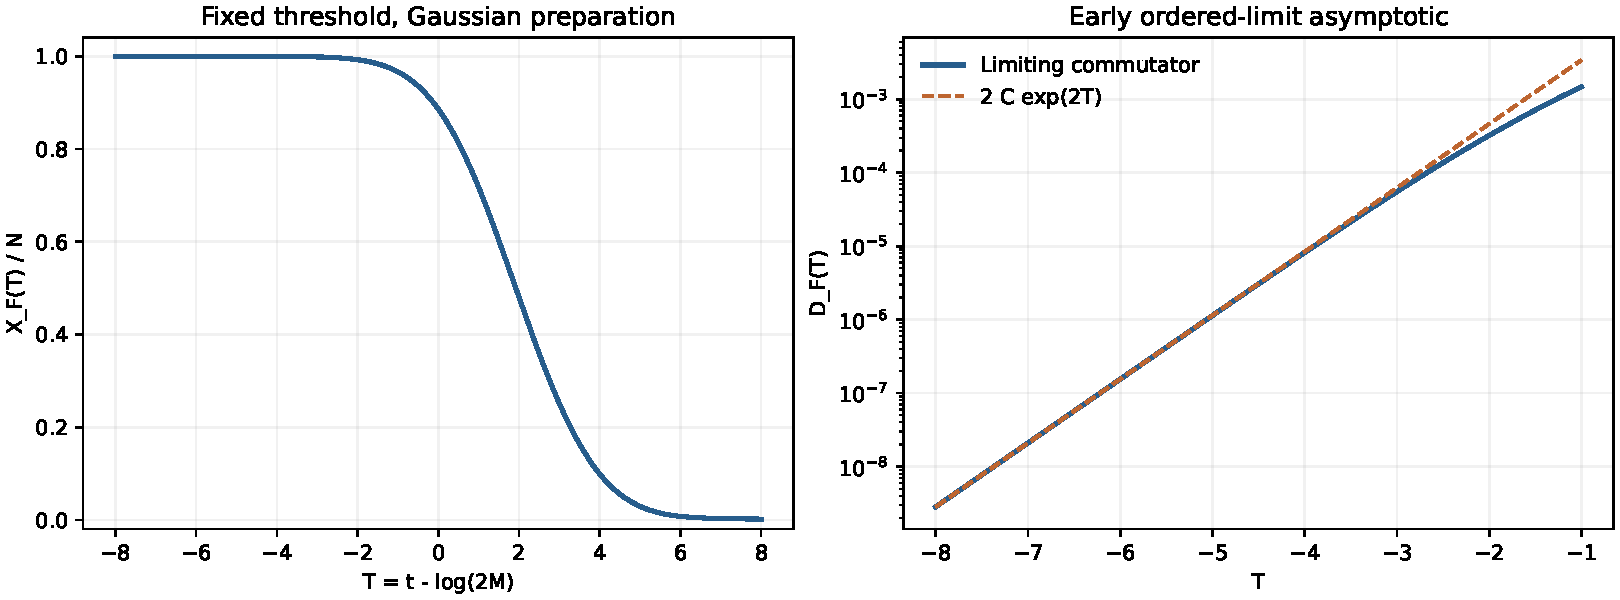
\includegraphics[width=.94\linewidth]{../results/stage3/preparation/fixed-curve.pdf}
 \caption{Fixed-threshold Gaussian limiting curve for $\nu=0.6$,
 $\sigma=1$. The right panel compares the commutator norm with its
 proven ordered-limit early asymptotic. Displayed curves have empirical
 quadrature checks; they are not finite-$M$ data.}
 \label{fig:prep-fixed}
\end{figure}

\section{A resolved moving-threshold curve}
\label{sec:movingcurve}
We now evaluate the full limiting integral of
Section~\ref{sec:preparation}, rather than constructing a curve from its
local corner coefficient. The model remains dS$_2$, $L=1$, proper
$SO^+(2,1)$, strict $G_N\to0$, BD free matter with two independent equal
principal-series species, a normalized vacuum external packet, fixed
proper Gaussian smearing, and the repeated moving projection $Q_M$.
Here $\pi_0(r)=\beta e^{-\beta r}$. The numerical example fixes
$\nu=0.6$, $\sigma=\beta=1$. All times use
$t_M=\log(2M)+T$, with $M\to\infty$ taken first.

\subsection{Splitting every transverse boundary}
Integrating the external excess $r$ exactly gives
\begin{equation}
 J_Q(\chi)=\iint_{\mathbb R^2} f_\chi(u)f_\chi(v)
 \exp\!\left[-\beta\max\left(0,-u-\frac\chi2,
                  -v-\frac\chi2,-u-v\right)\right]\dd u\dd v.
 \label{eq:mq-weight}
\end{equation}
This is still the hard projection, with no smoothing of its boundaries.
For fixed $u$, set
\begin{align}
 a_\chi(u)&=\max(0,-u-\chi/2),&
 b_\chi(u)&=\max(-\chi/2,-u),\notag\\
 E_\chi(s)&=\int_{-\infty}^s e^{\beta v}f_\chi(v)\dd v,&
 H_\chi(s)&=\int_s^\infty f_\chi(v)\dd v.
\end{align}
The maximum in \eqref{eq:mq-weight} is
$\max(a_\chi,b_\chi-v)$. Its two branches meet at $v=b_\chi-a_\chi$, so
\begin{equation}
 J_Q(\chi)=\int f_\chi(u)
 \left[e^{-\beta b_\chi}E_\chi(b_\chi-a_\chi)
       +e^{-\beta a_\chi}H_\chi(b_\chi-a_\chi)\right]\dd u.
 \label{eq:mq-slice}
\end{equation}
The outer panels split at $u=\pm\chi/2$, and each inner panel ends at
the actual moving boundary. No tensor rule is applied across a max fold.

As an independent geometric representation, use symmetry to restrict to
$v\le u$, and put $d_\chi(u)=\chi/2$ for $u\ge\chi/2$ and
$d_\chi(u)=u$ otherwise. Then
\begin{equation}
 J_Q(\chi)=2\int f_\chi(u)\left[
 e^{\beta d_\chi(u)}E_\chi\bigl(\min(u,-d_\chi(u))\bigr)
 +\one_{u>-d_\chi(u)}\int_{-d_\chi(u)}^u f_\chi(v)\dd v
 \right]\dd u.
 \label{eq:mq-ordered}
\end{equation}
Indeed, in this half-plane $-v-\chi/2\ge-u-\chi/2$; comparison with
$-u-v$ switches at $u=\chi/2$. Both implementations retain complex
$f_\chi$. They share the same special-function routine, so agreement
checks geometry and quadrature, not independent Gamma certification.

\subsection{Static normalization and stable small differences}
At $\chi=0$, the weight factorizes. With $k(w)=f_0(w)/(16\pi^3)$, define
\begin{align}
 g&=\int_0^\infty k(x)\dd x,&
 \ell&=\int_0^\infty k(-u)e^{-\beta u}\dd u,\notag\\
 m&=\int_0^\infty\!\int_0^\infty
       k(x)k(-u)e^{-\beta(u-x)_+}\dd u\dd x.
\end{align}
The two-step path norm and early crossed plateau are
\begin{equation}
 N_\infty^Q=g^2+g\ell+m+\ell^2,\qquad
 X_\infty^Q=(g+\ell)^2,\qquad
 \mathcal D_{\rm edge}=2(m-g\ell).
 \label{eq:mq-static}
\end{equation}
The last difference is computed directly as a positive integral with
weight $e^{-\beta(u-x)_+}(1-e^{-\beta\min(u,x)})$, using
\texttt{expm1}. The resulting values are
\begin{align}
 N_\infty^Q&\simeq0.007843474197608,\notag\\
 X_\infty^Q&\simeq0.007649270098482,\notag\\
 \mathcal D_{\rm edge}&\simeq0.0003884081982512.
 \label{eq:mq-static-values}
\end{align}
The independently evaluated $J_Q(0)/(256\pi^6)$ agrees with
$X_\infty^Q$.

For either subtraction width $a=1$ or $2$, let
\begin{equation}
 I_a(T)=\int e^{iT\chi}
 \left[A_Q(\chi)-\frac{iX_\infty^Q e^{-a\chi^2}}{2\pi\chi}\right]\dd\chi.
\end{equation}
The exact representations used in the numerical calculation are
\begin{align}
 \mathcal X_Q(T)&=\frac{X_\infty^Q}{2}
       \left[1-\operatorname{erf}\!\left(\frac{T}{2\sqrt a}\right)\right]
       +I_a(T),\notag\\
 \mathcal D_Q(T)-\mathcal D_{\rm edge}
   &=X_\infty^Q\left[1+\operatorname{erf}\!\left(\frac{T}{2\sqrt a}\right)\right]
       -2\operatorname{Re}I_a(T).
 \label{eq:mq-small-difference}
\end{align}
The second line avoids subtracting two plateau-size commutators. It
does not remove cancellation inside the Fourier integral. Unlike the
fixed protocol, $\mathcal X_Q$ need not be real: for example
$\mathcal X_Q(0)\simeq0.00691324056+0.00008422460\,i$.

\subsection{Numerical comparison with the corner prediction}
Composite Gauss--Legendre integration uses a transverse box
$[-10,10]^2$ and $\chi\in[-12,12]$, with a panel break at zero.
Transverse/Fourier orders are varied separately as
$(24,40)$, $(32,40)$ and $(24,64)$. The central Fourier panels have
width $1/2$. Both PV subtraction widths, both transverse representations
at selected frequencies, and transverse radii $8,10,12$ are recorded.
Twenty-five detailed times and a 257-point central curve retain full
complex values.
The maximum changes in the 25 complex correlators are approximately
$6.14\times10^{-18}$ under transverse refinement and
$2.08\times10^{-17}$ under Fourier refinement. Relative to the real
early plateau difference or the real late correlator, the largest
observed change is $1.90\times10^{-7}$. These are empirical differences
between rules, not rigorous accuracy estimates.

The actual integrals give dimensionless ratios to the leading coefficient
of Theorem~\ref{thm:prep-moving}, defined by
\[
 R_{\rm early}(s)=\frac{(\mathcal D_Q(-s)-\mathcal D_{\rm edge})s^3}{2B},
 \qquad R_{\rm late}(s)=\frac{\operatorname{Re}\mathcal X_Q(s)s^3}{B}.
\]
\begin{center}
\begin{tabular}{rcc}
\toprule
$|T|$ & $R_{\rm early}(|T|)$ & $R_{\rm late}(|T|)$\\
\midrule
16 & 0.74636 & 1.75824\\
32 & 0.85907 & 1.16537\\
64 & 0.92589 & 1.08068\\
128 & 0.96205 & 1.03962\\
\bottomrule
\end{tabular}
\end{center}
These approach the predicted value one without a
fitted time shift. Even at $|T|=128$, finite-$T$ corrections are several
percent; the leading asymptotic is not an exact finite-time curve.
At $T=-128$ the early difference is about $1.09044\times10^{-10}$,
and the absolute regular-integrand scale divided by half that signal
is about $7.28\times10^7$. Refinement comparisons must therefore be
reported relative to this small signal, not only to $N_\infty^Q$.

For real frequencies Euler's integral gives
$|f_\chi(w)|\le\Gamma(1/4)^4e^{-\pi w-w^2}$ at the stated $\sigma=1$.
If $G$ is the integral of this envelope and $g_R$ its tail outside
$[-R,R]$, then the omitted transverse region contributes at most
$2Gg_R$ to $J_Q(\chi)$, since the projection weight is at most one.
The outer Gaussian similarly controls the omitted real-frequency tail.
The archived bound expressions are evaluated in floating point, without
outward rounding. They are separate tail bounds, not a certified total
error for the subtracted PV quadrature. Order comparisons provide
empirical numerical support for the curve and the corner prediction.

\begin{figure}[htbp]
 \centering
 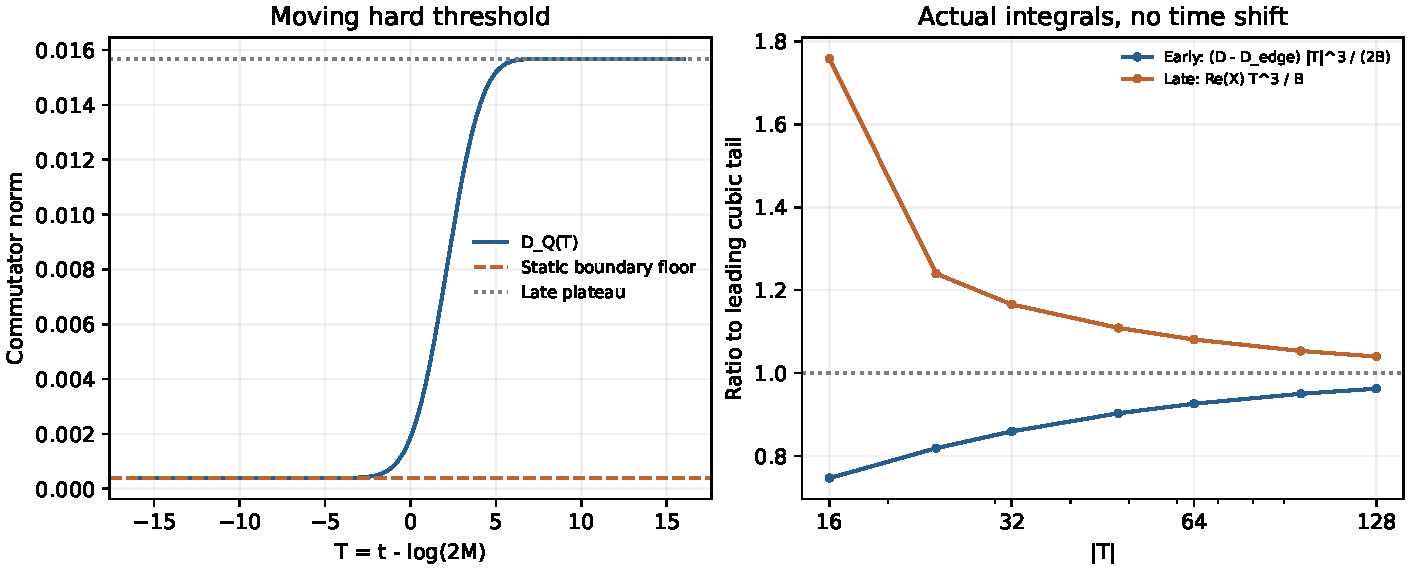
\includegraphics[width=.98\linewidth]{../results/stage3/moving-curve/moving-curve.pdf}
 \caption{Actual limiting integrals for the exponential packet and repeated
 moving hard threshold. The right panel compares independently computed
 time curves with the analytic corner coefficient; the coefficient was
 not used to generate the curves. This is ordered-limit data, not a
 finite-mass simulation or finite-$G_N$ calculation.}
 \label{fig:moving-curve}
\end{figure}

\section{Preparation endpoints, phases, and the real commutator}
\label{sec:densityendpoints}
We retain the state, free-matter algebra, projected Gaussian operators,
proper group, units, and strict-$G_N\to0$ assumptions of
Section~\ref{sec:movingcurve}. We change only the normalized external
excess density. The limit remains $M\to\infty$ at
$t_M=\log(2M)+T$, followed by large positive or negative $T$.
The endpoint Fourier expansion is standard (DLMF 2.3.4~\cite{DLMF}); the issue here
is which complex coefficient survives taking the real part of this
particular correlator. No priority claim is made.

\subsection{Gamma densities and a two-term corner expansion}
For a fixed integer $p\ge0$ and $\beta>0$, take
\begin{equation}
 \pi_p(r)=\frac{\beta^{p+1}}{p!}r^pe^{-\beta r}\one_{r\ge0}.
 \label{eq:dep-density}
\end{equation}
Write $J_p$ for \eqref{eq:prep-moving-domain} with this density.
The square-minus-triangle formula \eqref{eq:prep-triangle} still holds.
Let $J_{p,\rm sm}$ denote the reference obtained by replacing $L_+^2$
by $L^2$ inside the $r$ integral. Its exact difference is
\begin{equation}
 J_p(\chi)-J_{p,\rm sm}(\chi)
 =\one_{\chi<0}\int_0^{-\chi}\pi_p(r)(r+\chi)^2 B(r,\chi)\dd r.
 \label{eq:dep-difference}
\end{equation}
This reference is an algebraic device, not a different projection.
Define real constants
\begin{align}
 F_\nu&=f_0(0)=\left|\Gamma(1/4+i\nu/2)\right|^4,\notag\\
 q_\nu&=\operatorname{Re}\psi(1/4+i\nu/2),&
 H_\nu&=2q_\nu+\gamma_E+2\log2,\notag\\
 d_p&=\frac{\pi p-\beta(p+1)}{p+4},&
 S_p&=\frac{\beta^{p+1}F_\nu^2}{512\pi^7}.
 \label{eq:dep-coefficients}
\end{align}
Here $H_\nu$ is a scalar coefficient, distinct from the external-leg
function $H_\nu(x,y,z)$ of Section~\ref{sec:logtime}.

\begin{lemma}[Differentiated endpoint expansion]
For $h\downarrow0$,
\begin{equation}
 J_p(-h)-J_{p,\rm sm}(-h)
 =\frac{\beta^{p+1}F_\nu^2}{(p+3)!}h^{p+3}
       \left[1+h(d_p-2iq_\nu)+O(h^2)\right].
 \label{eq:dep-corner-two}
\end{equation}
The bracket is smooth in $h$ near zero, so the remainder has its
corresponding one-sided derivative bounds.
\end{lemma}
\begin{proof}
Set $r=h\rho$, $\chi=-h$, $0\le\rho\le1$. In the unit triangle
$s,t\ge0$, $s+t<1$, its two arguments become
\[
 u=h\left(\frac12-\rho+(\rho-1)s\right),\qquad
 v=h\left(\frac12-\rho+(\rho-1)t\right).
\]
At the origin the derivatives are
\begin{equation}
 \partial_w\log f_\chi(w)\big|_{0,0}=-\pi,\qquad
 \partial_\chi\log f_\chi(w)\big|_{0,0}=iq_\nu.
 \label{eq:dep-derivatives}
\end{equation}
The Gamma factors are even in $w$ at zero, while their four digammas
sum to $4q_\nu$. The Gaussian has no first derivative there.
The triangle has area $1/2$ and mean $s+t=2/3$, hence
\[
 B(h\rho,-h)=\frac{F_\nu^2}{2}
 \left[1+h\left(-2iq_\nu-\frac\pi3+\frac{4\pi}3\rho\right)
       +O(h^2)\right].
\]
Combining this with $e^{-\beta h\rho}$, use
\[
 \int_0^1\rho^p(1-\rho)^2\dd\rho
 =\frac{2p!}{(p+3)!},\qquad
 \frac{\int_0^1\rho^{p+1}(1-\rho)^2\dd\rho}
      {\int_0^1\rho^p(1-\rho)^2\dd\rho}=\frac{p+1}{p+4}.
\]
This gives \eqref{eq:dep-corner-two}. The rescaled integration domain
is compact and all Gamma arguments stay away from poles in a common
neighborhood of $h=0$. Differentiation under the integral proves the
claimed remainder control.
\end{proof}

\subsection{Taking the real part changes the leading power}
Let $\mathcal P_p(T)=X_{\infty,p}^Q$ for $T<0$ and zero for $T>0$;
this notation specifies the two asymptotic plateaux, not an additional
time-domain term in the experiment.
\begin{theorem}[Gamma-packet ordered-time tails]
For fixed $p\in\mathbb Z_{\ge0}$ and $\beta,\nu,\sigma>0$,
\begin{equation}
 \mathcal X_p(T)-\mathcal P_p(T)
 =S_p\left[\frac{-i}{(p+3)(iT)^{p+3}}
      +\frac{-H_\nu-id_p}{(iT)^{p+4}}\right]
      +O(|T|^{-p-5}),\qquad T\to\pm\infty.
 \label{eq:dep-complex-tail}
\end{equation}
Consequently, for $s\to+\infty$,
\begin{align}
 \mathcal D_p(-s)-\mathcal D_{{\rm edge},p}
 &=\frac{2(-1)^k S_p}{p+3}s^{-p-3}+O(s^{-p-4}),
       &&p=2k,\notag\\
 &=2(-1)^{k+1}S_p d_p\,s^{-p-4}+O(s^{-p-5}),
       &&p=2k+1.
 \label{eq:dep-real-tail}
\end{align}
If $p$ is odd and $\beta=\pi p/(p+1)$, the displayed real coefficient
vanishes; this theorem then supplies an $O(s^{-p-5})$ bound, not a
nonzero leading coefficient at that order.
\label{thm:dep-gamma}
\end{theorem}
\begin{proof}
The prefactor multiplying $J_p$ in the Fourier amplitude is
\begin{equation}
 P_\sigma(\chi)=\frac{2^{2i\chi}}{512\pi^7}
   \Gamma(-i\chi)\cosh(\pi\chi/2)e^{-\sigma^2\chi^2/2}.
 \label{eq:dep-prefactor}
\end{equation}
At $\chi=-h$ it equals
\[
 P_\sigma(-h)=\frac1{512\pi^7}
       \left[-\frac ih-\gamma_E-2\log2+O(h)\right].
\]
Thus the two nonsmooth amplitude terms, expressed in $h=-\chi>0$,
are
\begin{equation}
 \frac{S_p}{(p+3)!}\left[-ih^{p+2}
                   +(-H_\nu-id_p)h^{p+3}\right]\one_{h>0}.
 \label{eq:dep-amplitude}
\end{equation}
For a smooth cutoff equal to one at $h=0$, the endpoint transform of
$h^n$ under $e^{-iTh}$ has leading term $n!/(iT)^{n+1}$.
This follows by repeated integration by parts on the half-line, with
the same formula for either sign of real $T$. It is not an absolutely
convergent transform of an uncut polynomial.

For completeness, the needed global bounds follow from Euler's Gamma
integral and its logarithmic moments. All fixed real derivatives of
$f_\chi$ are bounded by a Gaussian in $w$ times a polynomial in $w$.
The square and rescaled-triangle terms and their derivatives have at
most polynomial growth in $r,\chi$; every $r$ moment of \eqref{eq:dep-density}
is finite. Multiplication by the outer Gaussian makes all one-sided
amplitude derivatives integrable at infinity. Subtracting the PV pole
$iX_{\infty,p}^Q e^{-\chi^2}/(2\pi\chi)$ removes the remaining zero
singularity. A local smooth cutoff separates
\eqref{eq:dep-amplitude} from a smooth rapidly decreasing part. The
differentiated Taylor remainder and one further integration by parts
give $O(|T|^{-p-5})$. The subtracted pole supplies the two plateaux,
up to Gaussian-small terms. This proves \eqref{eq:dep-complex-tail}.
Finally use
$\mathcal D_p=2(N_{\infty,p}^Q-\operatorname{Re}\mathcal X_p)$ and
$\mathcal D_{{\rm edge},p}=2(N_{\infty,p}^Q-X_{\infty,p}^Q)$.
The first coefficient in \eqref{eq:dep-complex-tail} is real for even
$p$ and purely imaginary for odd $p$, giving \eqref{eq:dep-real-tail}.
\end{proof}
For $p=0$ the leading term recovers Theorem~\ref{thm:prep-moving}.
The first two complex coefficients are independent of $\sigma$ at
fixed $\sigma>0$, because its Gaussian begins contributing at second
order at this corner. Remainders and useful time ranges are not uniform
as $\sigma$ varies.

For $\beta=1$, $p=1$ has a purely imaginary $T^{-4}$ term but a
real $T^{-5}$ correction. Since $d_1=(\pi-2)/5>0$, its early
$\mathcal D_1-\mathcal D_{{\rm edge},1}$ is negative. The $p=2$
early correction is also negative. Therefore
$\mathcal D_{\rm edge}$ is an early plateau, not a universal lower
bound on $\mathcal D(T)$. This is compatible with positivity of the
full commutator norm: its plateau is strictly positive. It also
precludes universal monotone growth from the early plateau across
these preparations.

\subsection{A support gap moves the singularity away from the PV pole}
Now take a fixed gap $g>0$ and
\begin{equation}
 \pi_g(r)=\beta e^{-\beta(r-g)}\one_{r\ge g}.
 \label{eq:dep-gap-density}
\end{equation}
The projection is still $Q_M$, not $Q_{M+g}$. Only the external state
has changed. The triangle correction begins at $\chi=-g$. Writing
$\chi=-g-h$, $r=g+h\rho$ gives
\[
 J_g(-g-h)-J_{g,\rm sm}(-g-h)
 =\frac{\beta f_{-g}(-g/2)^2}{6}h^3+O(h^4).
\]
This again has differentiated one-sided remainders. Now $P_\sigma$
is regular and nonzero at $-g$, so no zero-frequency pole lowers
the corner order.
\begin{proposition}[Gapped exponential packet]
Define the nonzero complex number
\begin{equation}
 C_g=\beta P_\sigma(-g)f_{-g}(-g/2)^2.
 \label{eq:dep-gap-coefficient}
\end{equation}
With the analogous early/late plateau notation,
\begin{align}
 \mathcal X_g(T)-\mathcal P_g(T)
   &=\frac{C_g e^{-igT}}{T^4}+O(|T|^{-5}),&&T\to\pm\infty,\notag\\
 \mathcal D_g(-s)-\mathcal D_{{\rm edge},g}
   &=-\frac{2\operatorname{Re}(C_g e^{igs})}{s^4}+O(s^{-5}),
      &&s\to+\infty.
 \label{eq:dep-gap-tail}
\end{align}
The constants are for fixed $g>0$; the expansion is not uniform as
$g\downarrow0$.
\label{prop:dep-gap}
\end{proposition}
\begin{proof}
Apply the same cutoff and derivative argument at $\chi=-g$.
The transform of $h^3$ supplies $6/(iT)^4=6/T^4$, and translation
supplies $e^{-igT}$. The smooth part at $\chi=0$ retains its PV pole
and therefore the usual plateaux. All external moments remain finite.
Gamma has no zeros and no pole at the arguments in
\eqref{eq:dep-gap-coefficient}, so $C_g\ne0$.
\end{proof}
The signed early correction thus has oscillatory sign changes along
sequences of arbitrarily early ordered-limit times. Removing density
near $r=0$ has not restored the fixed-threshold exponential: it has
displaced the nonsmooth endpoint. Taking $g\to0$ before the time
asymptotic requires a separate crossover analysis.

\subsection{Direct integral checks}
For \eqref{eq:dep-density}, the survival weight is
$e^{-\beta q}\sum_{j=0}^p(\beta q)^j/j!$ for $q\ge0$
(DLMF 8.4.8). The gapped exponential uses
$e^{-\beta(q-g)_+}$. In both cases $q$ is the actual max in
\eqref{eq:mq-weight}. The first implementation integrates polynomial
moments over exact slice domains; the second uses the survival
function directly on the symmetric half-plane. No endpoint coefficient
is used in generating the full curves.

The archived runs vary transverse/Fourier orders as $(24,40)$,
$(32,40)$, and $(24,64)$ for $p=1,2$ at $\beta=1$ and for
$g=\beta=1$. They keep $\nu=0.6$, $\sigma=1$, complex amplitudes,
and separate small real differences. Local corner integrals separately
test the two-term Taylor coefficient. Numerical diagnostics and their
precision limits are reported with the data; they do not independently
certify these proof drafts, priority, or a total quadrature error.

For the numerical parameters, $H_\nu\simeq-1.65594788424$ and the
early real coefficients multiplying $s^{-5}$ are approximately
$-1.62815710723\times10^{-4}$ for $p=1$ and
$-1.42621547371\times10^{-4}$ for $p=2$. The directly integrated
real corrections divided by these signed leading terms are
\begin{center}
\begin{tabular}{rcc}
\toprule
$s=|T|$ & $p=1$ & $p=2$\\
\midrule
16 & 0.65345 & 0.62126\\
32 & 0.78681 & 0.77729\\
64 & 0.8824 & 0.8800\\
\bottomrule
\end{tabular}
\end{center}
At $T=-64$, the actual corrections are about
$-1.3380\times10^{-13}$ and $-1.1689\times10^{-13}$, respectively.
The largest observed relative changes of the small real component over
the detailed times with $|T|\le64$ are $4.64\times10^{-4}$ and
$6.62\times10^{-4}$. At $|T|=128$, the signals are only a few
$10^{-15}$ and their observed changes rise to about $0.65\%$ and
$0.95\%$. Those samples are retained but excluded from the primary
quantitative table. The visible difference from unity is a finite-time
effect, much larger than the displayed empirical refinement differences.

For $g=1$, $C_g\simeq0.000479119472+0.000588336141\,i$.
The normalized signed oscillation in Figure~\ref{fig:dep-curves}
has maximum observed refinement change about $1.74\times10^{-5}$
over its 513 plotted times. Its remaining phase and amplitude corrections
are not removed by fitting. The survival weights in all three examples
are between zero and one, so the separate real-frequency and transverse
envelope bounds of Section~\ref{sec:movingcurve} continue to apply.
They still do not certify the total PV quadrature error. The archive
contains 384 diagnostics, full complex spectra, local-corner data, and
the reduced-precision far-time samples.
\begin{figure}[htbp]
 \centering
 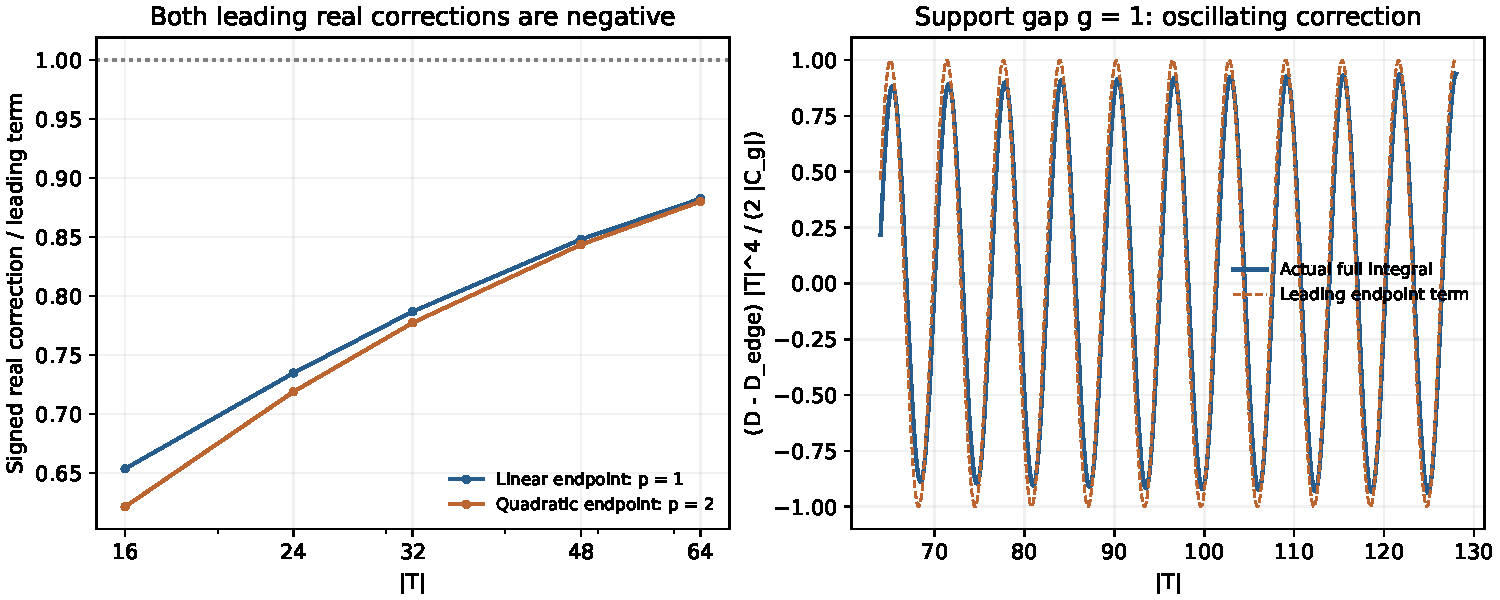
\includegraphics[width=.98\linewidth]{../results/stage3/density-endpoints/endpoint-curves.pdf}
 \caption{Actual full integrals versus endpoint predictions for
 $\nu=0.6$, $\sigma=\beta=1$. Left: ratios to the negative early
 $s^{-5}$ corrections for Gamma packets. Right: the signed early
 correction for a fixed support gap $g=1$, rescaled by $s^4/(2|C_g|)$,
 compared with $-\cos(\arg C_g+gs)$. These are empirical ordered-limit
 calculations, not finite-$M$ data.}
 \label{fig:dep-curves}
\end{figure}

\section{Keeping both branches at finite mass}
\label{sec:twobranch}
We retain the dS$_2$, $L=1$, proper-group, strict-$G_N\to0$ model,
BD vacuum, two equal independent principal-series species, fixed
$\nu,\sigma>0$, and the repeated projections of Section~9. The external
packet is normalized in exact energy. This section separates an identity
for the assembled leading kernel from its error relative to the exact
finite-mass correlator. All proof statements are author self-reviewed
drafts. The two branches originate in KL (B.41)--(B.50)~\cite{KL}; no
new gravitational interaction or priority claim is intended.

\subsection{Conjugate amplitudes with the actual projection}
Put $\ell=\log(2M)$, $T=t-\ell$, and $k=t+\ell=2\ell+T$.
For either protocol let $A_P(\chi)$ denote the integrated minus-branch
amplitude of Section~13, with the density replacements of Section~15
when appropriate. The plus-branch amplitude at the \emph{same}
real $\chi$ is $\overline{A_P(\chi)}$.
This is not the claim $A_Q(-\chi)=\overline{A_Q(\chi)}$, which generally
fails because the projection domain changes with $\chi$.
Indeed the pointwise identity, before any transverse integration, is
\begin{equation}
 \frac{H_\nu V_+}{\pi^3}e^{-\sigma^2\mathcal Q/2}
 =\frac{2^{-2i\chi}\cosh(\pi\chi/2)}{512\pi^7}
 e^{-\sigma^2\chi^2/2}f_{-\chi}(u)f_{-\chi}(v).
 \label{eq:tb-plus-factor}
\end{equation}
For example, the $c$-ratio numerator in $V_+$ contains
$c(1/2+i(x-y\pm\nu))$, and the denominator contains
$c(1/2-i(z\pm\nu))$. They cancel the corresponding oriented external
Gamma factors. The four remaining $x$ factors have common real part
$1/4$ and shift $-i\chi/4$, and likewise for $z$.
Since $f_{-\chi}(w)=\overline{f_\chi(w)}$ for real $\chi,w$, comparison
with (13.3) proves the identity. Multiplication by $\Gamma(i\chi)$
and integration against the same real density and region $D_{r,\chi}$
preserve conjugation.

Define the two-branch leading packet by
\begin{equation}
 X^{(2),P}_M(t)=\operatorname{PV}\int_{\mathbb R}
 \left[e^{iT\chi}A_P(\chi)
       +e^{ik\chi}\overline{A_P(\chi)}\right]\dd\chi.
 \label{eq:tb-definition}
\end{equation}
The two pole residues cancel before integration; for the Gamma and
gapped packets this is an ordinary integral of their combined amplitude.
For other fixed $L^1$ densities use the common approximation prescription
of Section~12. The superscript $(2)$ identifies a leading-kernel
quantity, not an exact 6j evaluation.
\begin{proposition}[Mirror identity]
With $X^P_\infty$ the real fixed-time crossed plateau,
\begin{align}
 X^{(2),P}_M(t)
 &=\mathcal X_P(t-\ell)+\overline{\mathcal X_P(-t-\ell)}-X^P_\infty,
 \label{eq:tb-mirror}\\
 D^{(2),P}_M(t)
 &:=2\bigl(N^P_\infty-\operatorname{Re}X^{(2),P}_M(t)\bigr)\notag\\
 &=\mathcal D_P(t-\ell)+\mathcal D_P(-t-\ell)
                         -\mathcal D_{{\rm edge},P}.
 \label{eq:tb-D}
\end{align}
Here $\mathcal D_{{\rm edge},F}=0$. In particular
$X^{(2),P}_M(-t)=\overline{X^{(2),P}_M(t)}$ and $D^{(2),P}_M$ is even.
\end{proposition}
\begin{proof}
Each Fourier integral in (16.2) is the corresponding $\mathcal X$
minus $X_\infty/2$. Complex conjugation changes the sign of the time
argument. Adding them proves (16.3), and taking real parts proves
(16.4). The same calculation works for every real smooth compact
cutoff before its removal, so also for the regularized definition.
\end{proof}
The fast-branch remainder relative to its delta limit is therefore
$\overline{\mathcal X_P(-k)-X^P_\infty}$, with no fitted time shift.
It retains the full preparation-dependent early tail.

\subsection{A compact estimate that does not differentiate the time phase}
Let $0\le r\le L$ and $|x|,|y|,|z|\le R$, with $L,R$ fixed.
Denote this box by $\Omega_{L,R}$. Set
\begin{equation}
 C^0_M(x,y,z)=\frac{H_\nu(x,y,z)}{\pi^3}
 \left[e^{i\ell\chi}\Gamma(i\chi)V_+
       +e^{-i\ell\chi}\Gamma(-i\chi)V_-\right],
 \quad \chi=x-y+z.
 \label{eq:tb-C0}
\end{equation}
The bracket is evaluated at its removable value when $\chi=0$.
\begin{lemma}[Uniform compact density error]
For $0<\epsilon<1/4$ and sufficiently large $M$, there is a constant
$C_{L,R,\epsilon}$ independent of $M$ and of all real $t$ such that
\begin{align}
 \sup_{\Omega_{L,R}}|\widetilde{\mathcal C}_M-C^0_M|
 &\le C_{L,R,\epsilon}\,e_\epsilon(M),\notag\\
 e_\epsilon(M)&=M^{-1+\epsilon}
       +\frac{1+\ell}{M}+\frac{(1+\ell)^2}{M^2}.
 \label{eq:tb-compact-error}
\end{align}
The same bound times the finite weighted volume controls the truncated
crossed integral, uniformly over all real physical times $t$.
\label{lem:tb-compact}
\end{lemma}
\begin{proof}
Use $\Lambda=M$ in Theorem~11.1. On the box,
\[
 s(M+\xi)-M=\xi-\frac{1}{8M}+O_{L,R}(M^{-2}),
 \qquad j(M+\xi)=1+O_{L,R}(M^{-2}).
\]
The common $-1/(8M)$ cancels in every label difference. The external
factor divided by $M$ differs from $H_\nu$ by $O_{L,R}(M^{-1})$.
The assembled bracket is $O_{L,R}(1+\ell)$ and its first offset
derivatives are $O_{L,R}((1+\ell)^2)$. To see this through $\chi=0$,
subtract its explicit sinc term (11.11); its smooth remaining
amplitudes multiply $e^{\pm i\ell\chi}$. Differentiating the sinc
costs at most $O(\ell^2)$. This controls the $O(M^{-2})$ change of
differences without differentiating the unknown exact remainder.
Multiplication by the external factor and the three Jacobians gives
(16.6). Crucially, both densities are compared in the \emph{same exact
energy coordinates}, then multiplied by the identical unit-modulus
factor $e^{it\chi}$. There is no $|t|$ loss in this comparison.
Bounded hard indicators can be retained in its ordinary compact integral.
\end{proof}
This improves the deliberately coarse phase-change argument in
Section~12. It does not supply bounds on $C_{L,R,\epsilon}$ as the box
grows with $M$.

\subsection{Uniform absolute approximation on the full time axis}
Let $A,B,b$ be the positive-envelope quantities in Section~9 and put
\begin{align}
 \tau_X(L,R)&=2A\sqrt{2A b(R/2)}
                  +A^2\int_L^\infty\pi_0(r)\dd r,\notag\\
 \tau_N(L,R)&=2A b(R/2)+A^2\int_L^\infty\pi_0(r)\dd r.
 \label{eq:tb-tails}
\end{align}
The external tail is a Gamma survival function or a shifted exponential
for the packets of Section~15, and $b$ is a Gaussian tail. Their
constants remain those of the analytic envelope, not certified numbers.
\begin{theorem}[Two-branch absolute approximation]
For either fixed protocol and every fixed normalized $L^1$ external
density, with fixed $\nu,\sigma>0$,
\begin{equation}
 \sup_{t\in\mathbb R}|X^P_M(t,0,t,0)-X^{(2),P}_M(t)|\longrightarrow0.
 \label{eq:tb-uniform-X}
\end{equation}
More precisely, for each fixed box and sufficiently large $M$,
\begin{align}
 \sup_t|X^P_M-X^{(2),P}_M|
 &\le C_{L,R,\epsilon}'e_\epsilon(M)+4\tau_X(L,R),\notag\\
 |N^P_M-N^P_\infty|
 &\le C''_{L,R}/M+2\tau_N(L,R).
 \label{eq:tb-cutoff-bound}
\end{align}
Consequently $\delta_M^P:=\sup_t|D^P_M(t)-D^{(2),P}_M(t)|\to0$.
No explicit rate for this supremum is claimed.
\label{thm:tb-uniform}
\end{theorem}
\begin{proof}
Truncate each ordered tree as in Proposition~9.1 and discard $r>L$.
The exact crossed error is at most $\tau_X$, uniformly in $M,t$.
The truncated two-branch expression satisfies the same mirror identity,
with truncated limiting curves $\mathcal X_{L,R}$ and plateau
$X_{\infty,L,R}$. These curves can first be defined with smooth cutoffs
and thresholds; the norm bounds allow their removal. Equivalently,
on this compact box the transverse integral has a locally Lipschitz
amplitude at $\chi=0$: moving any of the finitely many linear faces
changes a volume by $O(|\Delta\chi|)$, uniformly in bounded $r$, and
the remaining smooth integrand has bounded derivatives. Integration
against the $L^1$ density preserves this bound. Its pole-subtracted
PV thus exists, including the hard faces.

For each fixed argument $U$, take the logarithmic-time limit of the
exact full and truncated pairings. Their difference is at most
$\tau_X$, so $|\mathcal X_P(U)-\mathcal X_{L,R}(U)|\le\tau_X$
for \emph{every} real $U$. This gives a supremum bound without
interchanging a supremum and a convergence limit. The fixed-time limit
likewise gives $|X^P_\infty-X_{\infty,L,R}|\le\tau_X$.
The mirror identity now bounds the full-minus-truncated two-branch
expression by $3\tau_X$, independently of $M,t$. On the compact box
Lemma~\ref{lem:tb-compact} bounds the remaining exact-minus-leading
difference. This proves the first inequality in (16.9).

The positive ordered norms have excluded mass at most $\tau_N$.
Their compact one-step Gamma-ratio error is $O_{L,R}(M^{-1})$;
passing the same tail bound to the limit proves the second inequality.
For the fixed threshold the boundary has left the box once $M$ is
large enough. The moving threshold is identical in both integrands.
Finally, first choose $L,R$ large at fixed parameters, then take $M$
large. The commutator error is at most twice the crossed error plus
twice the norm error, proving the assertion.
\end{proof}
This theorem keeps both branches. Replacing the second branch by its
delta before applying the theorem would give a different approximation
and would discard the correction examined next.

\subsection{Which early signals can the fast branch compete with?}
Write $t=\ell-s$ so that $T=-s$ and $k=2\ell-s$. Assume $s,k\to\infty$.
Let $E_P(s)=\mathcal D_P(-s)-\mathcal D_{{\rm edge},P}$. Exactly,
\begin{equation}
 D^{(2),P}_M(\ell-s)-\mathcal D_{{\rm edge},P}=E_P(s)+E_P(k).
 \label{eq:tb-early-sum}
\end{equation}
For a Gamma packet with nonzero real coefficient $c_p$ in \eqref{eq:dep-real-tail}, put
$n=p+3$ for even $p$ and $n=p+4$ for odd $p$. Then
\begin{align}
 D^{(2),p}_M(\ell-s)-\mathcal D_{{\rm edge},p}
 &=c_p(s^{-n}+k^{-n})+O(s^{-n-1}+k^{-n-1}),\notag\\
 \frac{E_p(k)}{E_p(s)}
 &=\left(\frac{s}{k}\right)^n[1+O(s^{-1}+k^{-1})].
 \label{eq:tb-power-window}
\end{align}
In particular, for $s=a\ell$ with fixed $0<a<2$, the relative
fast-branch contribution tends to $(a/(2-a))^n$, not zero.
For positive physical times in this scaling take $0<a<1$.
Dropping the fast branch is relatively valid for these power tails
only when $s/k\to0$, equivalently $s=o(\ell)$ in the early regime.
The critical odd-$p$ density with $c_p=0$ is excluded.
At fixed $T$, the fast residual itself has a power of $\log M$;
this is a statement about the two-branch expression, not a determined
leading rate for the exact-minus-single-branch correlator.

For the fixed-threshold Gaussian, (13.6) instead gives, for $2<h<4$,
\begin{equation}
 D^{(2),F}_M(\ell-s)
 =2C_{\nu,\sigma}(e^{-2s}+e^{-2k})
      +O(e^{-hs}+e^{-hk}).
 \label{eq:tb-exponential-window}
\end{equation}
Its fast/slow ratio is $e^{-4t}[1+o(1)]$, so relative suppression
requires $t\to+\infty$ while $s\to\infty$. For a fixed gap,
\begin{equation}
 D^{(2),g}_M(\ell-s)-\mathcal D_{{\rm edge},g}
 =-2\operatorname{Re}\left[C_g\left(\frac{e^{igs}}{s^4}
                          +\frac{e^{igk}}{k^4}\right)\right]
    +O(s^{-5}+k^{-5}).
 \label{eq:tb-gap-window}
\end{equation}
Near zeros of the first oscillatory term only an envelope comparison
is meaningful; there is no uniform relative estimate there.

To transfer any displayed small signal to the exact finite-$M$
observable one must additionally have $\delta_M^P=o(s^{-n})$,
$o(e^{-2s})$, or $o(s^{-4})$, respectively. Theorem~16.3 proves
$\delta_M^P\to0$, not these explicit rates. It does imply existence
of some slowly growing windows. For a noncritical Gamma packet one
may take, for sufficiently large $M$,
\[
 s(M)=\min\{\sqrt\ell,(\delta_M^P)^{-1/(2n)}\},
\]
with the second entry interpreted as infinity at zero error. Then
$s\to\infty$, $s=o(\ell)$ and $\delta_M^P s^n\to0$.
For $F$ replace the second entry by
$\tfrac14\log(1/\delta_M^F)$, which gives
$\delta_M^F e^{2s}\to0$. These are existence constructions in terms
of an unknown error, not computable experimental windows. Quantifying
the growth of the compact constants in (16.9) is still required.

\subsection{Checks and the remaining finite-mass task}
The accompanying calculation verifies (16.1) directly from the original
$c$ ratios at high precision. It then reuses the frozen full projected
spectra of Sections~14--15, combines the two amplitudes before quadrature,
and compares with (16.3). Small early differences are formed from the
pole-subtracted integrals, not by subtracting two plateau-sized values.
The numerical records distinguish exact algebra, empirical quadrature,
and the still-uncomputed exact finite-mass remainder.

At $\nu=0.6$, $\sigma=\beta=1$, 300 empirical diagnostics pass.
For $s=\ell/2$ and $\ell=40$, the directly integrated fast/slow
real-correction ratios for $p=0,1,2$ are respectively $0.043283$,
$0.005156$, and $0.005305$. Their asymptotic targets are $1/27$,
$1/243$, and $1/243$. The three independent stored quadrature rules
give maximum relative changes of the small real quantities of
$4.14\times10^{-8}$, $4.30\times10^{-4}$, and $6.69\times10^{-4}$,
respectively; the gapped case gives $3.60\times10^{-6}$.
These are empirical refinement differences, not certified total errors.
The $p=2$ slow correction has not reached its negative asymptotic
regime at $\ell=16$; its negative fast/slow ratio there is retained
in the data. Figure~\ref{fig:tb-window} shows only $\ell\ge24$ to
resolve the subsequent approach, without treating earlier sign changes
as numerical failures.
\begin{figure}[htbp]
 \centering
 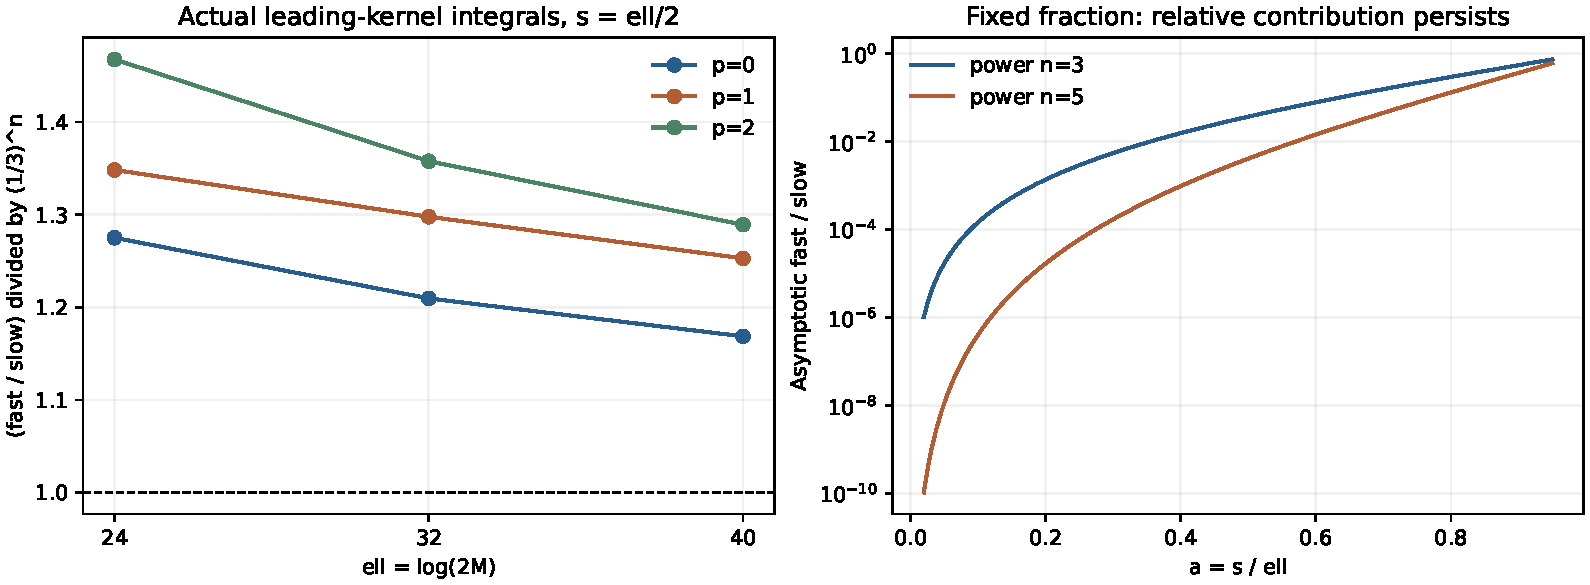
\includegraphics[width=.98\linewidth]{../results/stage3/two-branch/branch-window.pdf}
 \caption{Left: actual two-branch leading-kernel packet integrals, with
 $s=\ell/2$ and $k=3\ell/2$, normalized by the asymptotic fast/slow
 ratio. Right: the analytic limiting ratio for fixed $a=s/\ell$.
 Neither panel is an exact finite-$M$ 6j calculation.}
 \label{fig:tb-window}
\end{figure}

The next task is to bound $C_{L,R,\epsilon}'$ and $C''_{L,R}$ for an
explicit growing choice of $L,R$. Gaussian path tails suggest
$R$ of order $\sqrt{\log\log M}$ and exponential external tails suggest
$L$ of order $\log\log M$ for inverse-logarithmic target errors, but
these choices are not justified until the local constants are tracked.
No threshold smoothing loss is necessary for the compact two-branch
comparison; the positive-tail argument controls its removal globally.
Exact 6j packet calculations and total certified numerical errors remain
separate open work, as do finite-$G_N$ dynamics and a complete dual.

\section{Growing cutoffs and explicit asymptotic time windows}
\label{sec:growingbox}
We keep the states, projected Gaussian operators, exact-energy convention,
proper group and strict-$G_N\to0$ assumptions of Section~16. The issue is
the dependence of its compact constants on the offsets. We give deliberately
coarse analytic bounds, sufficient for explicit asymptotic windows. They
do not provide a certified numerical minimum mass for a prescribed accuracy.
The proofs below are author self-reviewed drafts, using the Euler and
Stirling estimates of DLMF~\cite[5.11, 15.6, 15.8, 2.3]{DLMF} and the
exact KL kernel~\cite{KL}; no priority claim is made.

\subsection{Constants in the Euler endpoint argument}
Let $Q_0\ge1$ bound the absolute values of the four real representation
offsets, with fixed $\nu>0$. The symbol $Q_0$ is unrelated to either
projection $Q_M$ or the Gaussian quadratic form $\mathcal Q$.
All the small parameters in Sections~10--11 then have imaginary parts
bounded by $c_0(1+Q_0)$, where $c_0$ is independent of $M,Q_0$.
Fix $0<\epsilon<1/4$. A complex tube of radius $\rho_\epsilon>0$
can be chosen independently of $Q_0$ so that every Euler endpoint real
part is between $1/4$ and $3/4$, the Gauss denominator real parts stay
near one, and $|\operatorname{Re}\delta|<\epsilon/4$.
The balanced identity remains exact. We take smaller nested disks when
removing the apparent $e=0$ and $\delta=0$ poles.

We will use an envelope
\begin{equation}
 \mathcal K(Q_0)=C e^{c Q_0}(1+Q_0)^d.
 \label{eq:gb-envelope}
\end{equation}
The fixed constants may be enlarged a finite number of times below;
they depend on $\nu,\epsilon$ and the tube margins, not on $Q_0$ or $M$.
Products and finite sums of such envelopes have the same form.

\begin{lemma}[Parameter-dependent endpoint bounds]
For the four KL hypergeometric factors in Section~11, the endpoint
remainder in \eqref{eq:endpoint-two-branch}, away from the small pole
disks, is bounded by
\begin{equation}
 \mathcal K(Q_0) M^{-1+\epsilon/4},
 \qquad M\ge C_0(1+Q_0)^2.
 \label{eq:gb-endpoint-bound}
\end{equation}
The same envelope class controls the required finite derivative norms
of the endpoint amplitudes. The constants and the large-mass threshold
are uniform over the indicated growing offset boxes.
\label{lem:gb-endpoint}
\end{lemma}
\begin{proof}
There are four separate estimates, with fixed differentiation order.

First, Gamma functions and their reciprocals on fixed vertical strips,
away from the finitely many poles in those strips, are bounded by an
exponential in the imaginary part times a polynomial. Stirling's formula
on the tails and compactness on the bounded part give this bound; fixed
derivatives obey it as well. Thus every small-parameter Gamma product,
connection coefficient $G_\pm$, and $c$ ratio off the pole disks is
bounded by \eqref{eq:gb-envelope}. The pole distance is fixed by
$\rho_\epsilon$, not by $Q_0$.

Second, for $Z=\pm i\lambda$, $\lambda$ proportional to $M$, and shifts
$|a|,|b|\le c_1(1+Q_0)$ with bounded real parts, the sectorial Stirling
remainder gives
\begin{align}
 \frac{\Gamma(Z+a)}{\Gamma(Z+b)}Z^{b-a}&=e^{E(Z;a,b)},\notag\\
 |E(Z;a,b)|&\le C_1(1+Q_0)^2/M,
 \qquad M\ge C_0(1+Q_0)^2.
 \label{eq:gb-gamma-ratio}
\end{align}
Here $E$ is defined using the analytic log-Gamma branch in the fixed
sector about $\pm i\mathbb R_+$, rather than the principal logarithm
of the final ratio. To see the bound directly, write
\[
 E=\int_b^a[\psi(Z+z)-\log Z]\dd z.
\]
On the joining segment $|Z+z|\asymp M$ and its argument stays away
from the negative real axis. The digamma expansion with sectorial
remainder bounds its integrand by $C(1+Q_0)/M$; the segment length is
$O(1+Q_0)$. Exponentiating gives a relative error bounded by
$C(1+Q_0)^2/M$ after increasing $C_0$. This derives a growing-shift
estimate, rather than substituting growing parameters into a fixed-shift
ratio formula. Factors such as $Z^{i y}$ cost at most $e^{C Q_0}$.

Third, all Gauss functions needed near either endpoint have an Euler
integral with real positive bases. For $0\le z\le z_*<1$,
$\operatorname{Re}B,\operatorname{Re}(C-B)>0$, and fixed $j\le5$,
the ordinary Gauss function obeys
\begin{align}
 |\partial_z^j{}_2F_1(A,B;C;z)|
 &\le |(A)_j|\left|\frac{\Gamma(C)}{\Gamma(B)\Gamma(C-B)}\right|
 \mathrm B(\operatorname{Re}B+j,\operatorname{Re}(C-B))\notag\\
 &\hspace{12mm}\times
 (1-z_*)^{-\max(\operatorname{Re}A+j,0)}.
 \label{eq:gb-euler-derivative}
\end{align}
This follows by differentiating Euler's integral: $t,1-t,1-zt$ are
positive, so their imaginary exponents have modulus one. It uses the
ordinary function, with the $\Gamma(C)$ restored from DLMF 15.6.1.
On the tube, the needed $(A,B;C)$ are $(b,d;g)$,
$(b,d;1-\delta)$ and $(g-b,g-d;1+\delta)$; all satisfy the stated
real-part conditions with fixed margins. Their derivative bounds have
form \eqref{eq:gb-envelope}. Near $w=0$ apply the latter two to
$z=1-e^{-w}$ on $0\le w\le1$; for $w$ away from zero apply the first
to $z=e^{-w}$.

Fourth, in \eqref{eq:endpoint-J}, $h(z)=(1-e^{-z})/z$ is positive
on the real half-line, $h(z)\asymp(1+z)^{-1}$, and its logarithmic
derivatives of any fixed positive order are bounded there. Direct
differentiation of $J$ therefore gives, for $j\le5$,
\begin{equation}
 |J^{(j)}(w)|\le C_j(1+Q_0)^{d_j}(1+w)^{d_j}e^{-w/4}.
 \label{eq:gb-J-bound}
\end{equation}
The $t$ weights remain integrable with fixed endpoint margins.
For $w\le1$, the same bounds apply to the smooth factors multiplying
$w^{a-1}$ and $w^0$ in the connection expansion, with
$a=1-\delta$. Their first Taylor remainders have respective forms
$w^a R_1(w)$ and $wR_2(w)$, with derivatives through order four bounded by
$\mathcal K(Q_0)$. Choose a smooth cutoff at zero once and for all,
independent of the parameters. Splitting at $w=1/|Z|$ and integrating
by parts four times on dyadic intervals gives transform bounds
$\mathcal K(Q_0)|Z|^{-\operatorname{Re}a-1}$ and
$\mathcal K(Q_0)|Z|^{-2}$. Differentiating $w^a$ only introduces
fixed-degree polynomials in $a$; the dyadic sums are uniform because
$\operatorname{Re}a$ stays near one. The exponentially decreasing
part away from zero has four integrable derivatives, with the same
envelope. The leading transforms are the Abel boundary values
$\Gamma(a)Z^{-a}$ and $Z^{-1}$, with their cutoff errors handled by
the same integrations by parts.

Finally, \eqref{eq:gb-gamma-ratio} controls the normalization
$\mathcal N_M\mathrm B(\alpha,\beta)$ in Section~10. Multiplying
the transform estimates by it, including its relative error, gives
\eqref{eq:gb-endpoint-bound}. No derivative order grows with $Q_0$.
\end{proof}

\subsection{Assembly and the growth of the compact constants}
\begin{proposition}[Growing-box density control]
There are $C,c,d,C_0>0$, for each fixed $\nu,\sigma,\epsilon$, such
that the compact constants in \eqref{eq:tb-cutoff-bound} may be chosen as
\begin{equation}
 C'_{L,R,\epsilon}+C''_{L,R}
 \le C e^{c(L+R)}(1+L+R)^d,
 \qquad M\ge C_0(1+L+R)^2.
 \label{eq:gb-compact-growth}
\end{equation}
The estimate retains the hard moving threshold. For $F$ one also
requires $M-R>m_*$, which holds eventually for the choices below.
\label{prop:gb-growth}
\end{proposition}
\begin{proof}
For representation offsets bounded by $Q_0$, the exact beta-like
prefactors have relative Gamma-ratio error
$\mathcal K(Q_0)/M$, and size
$\mathcal K(Q_0)M^{-1+\epsilon/4}$ off the apparent poles.
Lemma~\ref{lem:gb-endpoint}, the exact cancellation (11.6), and the
leading coefficients (11.7) consequently give
\begin{equation}
 |S-S_M^0|\le\mathcal K(Q_0)M^{-2+\epsilon}
 \label{eq:gb-raw-bound}
\end{equation}
there, leaving room in $\epsilon$ for the fixed tube margins.
The exact triple-integral holomorphy argument of Section~11 uses
real parts of exponents only. Those margins are independent of the
real offsets; hence its complex tube need not shrink with $Q_0$.
Use fixed-radius disks in $e,\delta$ at their intersections. Their
boundary stays in a box enlarged by a constant, on which the envelope
has the same form. Maximum modulus transfers \eqref{eq:gb-raw-bound}
inside. A pointwise choice of these disks has uniformly bounded overlap;
one does not multiply the bound by an uncontrolled covering constant.
Other Gamma arguments stay near real part $1/2$, so no new poles are
encountered on enlarging the real offsets.

The eight large external Gamma factors satisfy the same growing-shift
Stirling estimates. Their exponentially large mass factors cancel
the hyperbolic prefactor exactly at leading order, as in (11.14).
The remaining small Gamma factors and fixed offset derivatives have
envelope \eqref{eq:gb-envelope}. Thus $F_M/M-H_\nu$ is bounded by
$\mathcal K(Q_0)/M$; the same type of bound applies to the one-step
positive-kernel error. Hyperbolic errors are exponentially small for
$M\ge C_0(1+Q_0)^2$ and are absorbed in these estimates.

In exact-energy coordinates $|\xi|\le L+R$, Taylor expansion gives
\[
 s(M+\xi)=M+\xi-\frac1{8M}
                   +O((1+L+R)M^{-2}).
\]
The Jacobians have uniform $O(M^{-2})$ error when $M>2(L+R+1)$.
After removal of the pole, the first derivatives of the leading bracket
are bounded by $\mathcal K(Q_0)(1+\log(2M))^2$; this follows either
by its explicit sinc subtraction or the small-Gamma bounds above.
The argument of Lemma~16.2 now proves its density bound with an
envelope of the stated form, taking $Q_0=1+L+R$ and enlarging the
constants for fixed $\nu$. Compact volume factors add only a polynomial.
The external density contributes its mass, at most one, rather than
its supremum or derivatives. The Gaussian has modulus at most one.
For the ordered norms, apply the same positive one-step estimate twice.
No growing time seminorm or threshold smoothing constant is introduced.
\end{proof}

\subsection{An explicit cutoff choice for exponential-moment packets}
We now assume a fixed positive exponential moment:
\begin{equation}
 B_0:=\int_0^\infty e^{\beta_0r}\pi_0(r)\dd r<\infty,
 \qquad \beta_0>0.
 \label{eq:gb-moment}
\end{equation}
All fixed Gamma and shifted-exponential packets used above satisfy this,
for example with $\beta_0=\beta/2$; their $B_0$ are respectively
$2^{p+1}$ and $2e^{\beta g/2}$. This extra assumption is not made for
the arbitrary $L^1$ packets of Theorem~16.3.

\begin{theorem}[Rate and asymptotic cutoffs]
For a packet satisfying \eqref{eq:gb-moment}, both protocols obey,
for every fixed $q>0$,
\begin{equation}
 \delta_M^P:=\sup_{t\in\mathbb R}|D_M^P(t)-D_M^{(2),P}(t)|
 =O_q\bigl(\ell^{-q}\bigr),\qquad \ell=\log(2M).
 \label{eq:gb-log-rate}
\end{equation}
The same statement holds separately for the crossed error and the norm
error. An explicit admissible cutoff choice, for sufficiently large $M$, is
\begin{equation}
 L_M=\frac{q+2}{\beta_0}\log\ell,
 \qquad R_M=\sqrt{\frac{8(q+2)}{\sigma^2}\log\ell}.
 \label{eq:gb-explicit-cutoffs}
\end{equation}
There is also a positive mass-power rate $\delta_M^P=O(M^{-\kappa})$
for some $\kappa>0$ depending on the envelope constants and the packet.
We do not evaluate a numerical value of $\kappa$ here.
\label{thm:gb-rate}
\end{theorem}
\begin{proof}
Markov's inequality gives $\Pr(r>L)\le B_0e^{-\beta_0L}$.
For $R\ge1$, the Gaussian envelope of Section~9 gives
\[
 b(R/2)\le C e^{-\sigma^2R^2/4},\quad
 \tau_X+\tau_N\le C\{e^{-\sigma^2R^2/8}+e^{-\beta_0L}\}.
\]
With \eqref{eq:gb-explicit-cutoffs}, both tails are
$O(\ell^{-q-2})$. Write $Q_0=1+L_M+R_M=O_q(\log\ell)$.
The compact term in Theorem~16.3 and
Proposition~\ref{prop:gb-growth} is then at most
\[
 C_q\ell^{a_q+o(1)}
 \left[M^{-1+\epsilon}+\frac{1+\ell}{M}
                        +\frac{(1+\ell)^2}{M^2}\right],
\]
for a finite constant $a_q$. For each fixed $q$ this is smaller than
every inverse power of $\ell$, and $M\ge C_0Q_0^2$ holds eventually.
This proves \eqref{eq:gb-log-rate}, with no exchange of a fixed-box
limit and a growing box.

For the last assertion set $\epsilon=1/8$, let $c$ be the enlarged
coefficient in \eqref{eq:gb-compact-growth}, and put
\[
 \kappa=\frac{\beta_0}{8(c+\beta_0)},\quad
 L_M=\frac{\log M}{4(c+\beta_0)},\quad
 R_M=\sqrt{\frac{16\kappa}{\sigma^2}\log M}.
\]
Both tails are $O(M^{-2\kappa})$. The compact term is
$M^{-7/8+c/[4(c+\beta_0)]+o(1)}$, which is $O(M^{-\kappa})$
since $\kappa\le1/8$. The other terms are smaller; the required
large-mass condition still holds. The constants $c,C_0$ have analytic
existence bounds above but have not been numerically certified.
\end{proof}

\subsection{Consequences for the exact finite-mass observable}
Let $c_p\ne0$ be the real coefficient in \eqref{eq:dep-real-tail},
and $n=p+3$ for even $p$, $n=p+4$ for odd $p$. All density, field,
Gaussian and projection parameters are fixed in the following limits.
For every fixed $0<\alpha<1$, the \emph{exact} commutator satisfies
\begin{equation}
 D_M^p(\ell-\ell^\alpha)-\mathcal D_{{\rm edge},p}
 =c_p\ell^{-\alpha n}
  \left[1+O\left(\ell^{-\alpha}
                         +\ell^{-n(1-\alpha)}\right)\right].
 \label{eq:gb-gamma-window}
\end{equation}
In particular $s=\sqrt\ell$, which was not justified by Section~16
alone, is now an explicit asymptotic window. The signed coefficient
remains negative for $p=1,2$, $\beta=1$.
For a fixed fraction $0<a<2$ one instead obtains
\begin{equation}
 D_M^p((1-a)\ell)-\mathcal D_{{\rm edge},p}
 =c_p\ell^{-n}\{a^{-n}+(2-a)^{-n}\}
                         +O(\ell^{-n-1}).
 \label{eq:gb-gamma-fraction}
\end{equation}
This estimate is uniform on closed subintervals of $0<a<2$.
It retains both tails, including for positive physical time $a<1$.
For fixed physical $t$ in a bounded interval, it implies
\begin{equation}
 D_M^p(t)-\mathcal D_{{\rm edge},p}
 =2c_p\ell^{-n}+O(\ell^{-n-1}).
 \label{eq:gb-fixed-time-rate}
\end{equation}
For bounded $T$ at the positive logarithmic-time transition, it also gives
\begin{equation}
 D_M^p(\ell+T)-\mathcal D_p(T)
 =c_p(2\ell+T)^{-n}+O(\ell^{-n-1}).
 \label{eq:gb-fixed-T-rate}
\end{equation}
The critical odd-$p$ case with $c_p=0$ is excluded from these leading
coefficient statements.

For $F$, every fixed $b>0$ and $2<h<4$ give a different explicit window:
\begin{equation}
 D_M^F(\ell-b\log\ell)
 =2C_{\nu,\sigma}\ell^{-2b}
                  [1+O_h(\ell^{-(h-2)b})].
 \label{eq:gb-F-window}
\end{equation}
These formulas follow by inserting the Section~13--15 tails in the
mirror identity and choosing $q$ in \eqref{eq:gb-log-rate} larger than
the power being resolved. For \eqref{eq:gb-gamma-window}, the fast tail
relative to the slow one is $O(\ell^{-n(1-\alpha)})$; for
\eqref{eq:gb-F-window} it is exponentially small in $\ell$.
No unknown $\delta_M$ appears in the time choices.

For a fixed gap $g>0$, \eqref{eq:tb-gap-window} transfers to the exact
$D_M^g$ with its displayed $O(s^{-5}+k^{-5})$ error whenever $s,k$
are fixed positive powers of $\ell$ or fixed fractions away from zero.
This is an absolute envelope result. A relative statement still requires
separation from zeros of the relevant oscillatory combination, and the
estimate is not uniform as $g\downarrow0$.

The asymptotic window shapes are explicit, but these theorems do not
give a numerical mass at which a chosen percentage accuracy begins.
They are restricted to the stated free-matter, $G_N\to0$ model and do
not identify a finite-gravity chaos exponent. In particular the
$M^{-4}$ mirror correction for $F$ at fixed $T$ need not be the leading
exact correction; the above error bound need not resolve that power.

\subsection{Diagnostic scope and next physical comparison}
The new diagnostics check the shifted Gamma ratios on growing-parameter
fixtures, the explicit Euler derivative inequality and exact-energy
coordinate estimates. These probe the ingredients and conventions of
the proof. They do not certify its supremum constants, perform a full
finite-$M$ 6j packet integration, or independently validate the proof.
Previously frozen limiting spectra are not recomputed.

The saved run contains 290 checks at 80 decimal digits, with 110-digit
Gamma-ratio cross-checks. On the recorded shifts up to $Q_0=64$, the
largest $M|E|/(1+Q_0)^2$ is about $0.080004$; this is a sampled
quantity, not the universal constant in \eqref{eq:gb-gamma-ratio}.
The largest sampled ratio of a Gauss derivative to its Euler-integral
bound is about $0.883322$. The energy-coordinate and normalized tail
inequalities are checked separately. No finite collection of these
values proves the growing-box supremum estimate.

With the explicit asymptotic window established at this level, the next
physical step is a matched finite-$G_N$ comparison. The external state,
projection, proper time, normalization, matter representation and contour
must agree before the current preparation effects can be compared with
a genuine gravitational interaction or a microscopic candidate.
Numerically useful error constants and exact finite-mass packet checks
remain a separate validation task.


\section{Open questions}
The weak realization fixes the space and the order of regulation.
Section~\ref{sec:position} removes auxiliary position and group cutoffs
for the creation pairing on explicit test seeds and arbitrary physical
inputs. Section~\ref{sec:annihilation} identifies annihilation as an
integrated mode limit on all physical inputs and as an absolute uncut
position formula on seed inputs. Pointwise convergence and absolute
position formulas for arbitrary physical inputs remain open. The Gaussian
proper-time smearing and observer threshold have not been removed.

Two further questions are central to the original holographic objective.
First, Sections~\ref{sec:logtime} and \ref{sec:preparation} give the
logarithmic-time limit and distinguish the fixed-protocol exponential
early correction from an inverse-cubic hard-boundary correction for an
exponential packet.
Section~\ref{sec:twobranch} retains both oscillatory branches and
proves uniform absolute approximation on the full time axis. Its
mirror identity determines the fast-branch tail.
Section~\ref{sec:growingbox} supplies their exponential-polynomial
growth bounds and explicit asymptotic windows for packets with a
positive exponential moment. A numerically certified onset mass and
full exact finite-mass packet checks remain open.
Section~\ref{sec:densityendpoints} classifies the stated integer-order
Gamma densities and gapped exponential packets. General densities,
degenerate real coefficients, and a uniform gap-closing crossover still
require separate analysis. Section~\ref{sec:movingcurve} supplies a numerically
resolved moving-protocol curve for the exponential packet, with empirical
quadrature diagnostics rather than certified total error bars.
The constant source
time-origin discrepancy is now isolated algebraically, but is not an
author-confirmed correction.
Second, a finite-$G_N$ or microscopic comparison must
match states, spectral weights, time conventions, external legs, and
integration contours in a common parameter regime. The results here do not
settle either question. The known noncrossed large-mass expansion and the
finite-$G_N$ comparison notes remain separate parts of the research project.

\appendix
\section{Observer wave packets and spectral normalization}
\label{app:normalization}
This appendix supplies the positive/negative frequency normalization without
formally multiplying generalized eigenfunctions and delta functions.
Fix $k=|n|$, $h=k+1/2$, and $r(s)=s\tanh\pi s$. In the phase convention
of~\cite[(3.11), (4.9), (A.5)--(A.6)]{KL},
\begin{align}
 v_s(t)&:=\sqrt{\cosh t}\,\Psi_n^s(t,0)
 =N_k(s)\cosh^h t\,
 \mathbf F(h-is,h+is;k+1;z(t)),\\
 z(t)&=\frac{1-i\sinh t}{2},\\
 N_k(s)&=\sqrt{\frac{r(s)}{\pi}}\,
 e^{i\phi_{-k,s}/2}
 \frac{(1-i)(2i)^{-k}\Gamma(1/2-is)}
      {2\sqrt{2\cosh\pi s}\,\Gamma(1/2-k-is)}.
\end{align}
Here $\mathbf F={}_2F_1/\Gamma(c)$ and the half phase is chosen smoothly
and compatibly with the $n\leftrightarrow-n$ relation. Gamma recurrence
gives
\begin{equation}
 |N_k(s)|^2=\frac{r(s)2^{-2k}}{4\pi^2}
                         |\Gamma(h+is)|^2.
\end{equation}
For $t=\epsilon\tau$, $\epsilon=\pm1$, $\tau>0$, set $x=e^{-\tau}$.
The identity $-z(\epsilon\tau)=i\epsilon(1+i\epsilon x)^2/(4x)$ and
the hypergeometric connection formula~\cite[15.8.2]{DLMF} give
\begin{align}
 v_s(\epsilon\tau)&=\sum_{\sigma=\pm1}
       A_{\epsilon\sigma}(s)e^{i\sigma s\tau}
       M_{\epsilon\sigma}(x,s),\\
 A_{\epsilon\sigma}(s)&=B_\sigma(s)
          e^{-i\epsilon\pi h/2}e^{-\epsilon\sigma\pi s/2},\\
 B_\sigma(s)&=
 N_k(s)2^{h-2i\sigma s}
 \frac{\Gamma(2i\sigma s)}
      {\Gamma(h+i\sigma s)\Gamma(1/2+i\sigma s)},\\
 M_{\epsilon\sigma}(x,s)&=(1+x^2)^h
 (1+i\epsilon x)^{-2q_\sigma}
 {}_2F_1\left(q_\sigma,\tfrac12-i\sigma s;1-2i\sigma s;
       \frac{4i\epsilon x}{(1+i\epsilon x)^2}\right),\\
 q_\sigma&=h-i\sigma s.
\end{align}
The linear terms in the last expression cancel, so $M=1+x^2Q$ with
$Q$ analytic near $x=0$ on every compact positive spectral interval.
For fixed spectral and time derivative orders,
$|\partial_s^j\partial_\tau^l(M-1)|\le Ce^{-2\tau}$ for
$\tau\ge\log32$. Including the phase in the differentiated remainder
adds a factor $(1+\tau)^j$.
Thus $\int f(s)v_s(t)\dd s$ is Schwartz for $f\in\Cc((0,\infty))$.

The standard gamma moduli give
\begin{equation}
 |\Gamma(2is)|^2=\frac{\pi}{2s\sinh2\pi s},\qquad
 |\Gamma(1/2+is)|^2=\frac{\pi}{\cosh\pi s},\qquad
 |B_\sigma(s)|^2=\frac{1}{8\pi^2\cosh\pi s}.
 \label{eq:B-modulus}
\end{equation}
Now use the unitary radial variable $r_s(t)=\sqrt{2\pi}\,v_s(t)$ and
write $W_f=\int r_s f(s)\dd s$. Its Schwartz property and differential
equation imply
\begin{equation}
 e^{-iTH_k}W_f=W_{e^{-iTs^2}f}.
\end{equation}
As $T\to+\infty$, on each half-axis only the $\sigma=+$ outgoing
free packet remains. The $\sigma=-$ phase has no stationary point there,
and repeated spectral integration by parts bounds its $L^2$ norm by a
quantity tending to zero. The exponentially small Jost remainder tends
to zero on compact positions by nonstationary phase, and its tail is
uniformly $L^2$ dominated. The outgoing packet restricted to that half-axis
has the full-line Fourier norm in the limit; its omitted half-line is
again nonstationary. Plancherel therefore gives the packet Gram density
\begin{equation}
 4\pi^2\sum_{\epsilon=\pm1}
       \overline{A_{\epsilon,+}(s)}A'_{\epsilon,+}(s).
 \label{eq:packet-gram}
\end{equation}
For two positive columns, \eqref{eq:B-modulus} makes this density one.
For the negative-frequency column,
$A'_{\epsilon,+}=(-1)^nA_{-\epsilon,+}$. Its cross density is
\begin{equation}
 8\pi^2(-1)^n|B_+(s)|^2\cos(\pi h)=0.
\end{equation}
The negative column has the same unit norm. Different $n$ are already
orthogonal in $\theta$.

Finally the two asymptotic coefficient columns at $+\infty$ have determinant
\[
 -2(-1)^nB_+B_-\sinh\pi s\ne0.
\]
They span the two-dimensional
continuous solution space and are a smooth invertible change of basis
from the scattering modes on every compact positive interval. The bound
modes are orthogonal to these packets by the self-adjoint radial spectral
decomposition. This proves the full continuous normalization and
completeness needed in Section~\ref{sec:physical}; it makes no assertion
that the entire position representation lacks discrete series.

\section{Local vertex conventions and the crossed prefactor}
\label{app:vertex}
We distinguish the vertex reconstructed from the mode integral from the
literal expression in (A.7) of~\cite{KL}. This appendix fixes the convention
used in \eqref{eq:local-mode}; it is not an author-confirmed erratum.
Set $r_j=s_j\tanh\pi s_j$, $c_j=\cosh\pi s_j$, and define
\begin{align}
 G_4(s_1,s_2,s_3)
 &=\Gamma\!\left(\tfrac14+\tfrac i2(-s_1+s_2+s_3)\right)
   \Gamma\!\left(\tfrac14+\tfrac i2(-s_1-s_2+s_3)\right)\notag\\
 &\quad\times
   \Gamma\!\left(\tfrac14+\tfrac i2(-s_1+s_2-s_3)\right)
   \Gamma\!\left(\tfrac14+\tfrac i2(s_1+s_2+s_3)\right),\\
 D(s_1,s_2,s_3)
 &=\Gamma(1/2-is_1)\Gamma(1/2+is_2)\Gamma(1/2+is_3).
\end{align}
Then the reconstructed vertex is
\begin{equation}
 \mathcal V^{s_1}_{s_2,s_3,\mathrm{rec}}
 =e^{-i\pi/4}\frac{c_1\sqrt{r_1r_2r_3}}
                    {8\pi\sqrt{c_1c_2c_3}}\frac{G_4}{D}
 =\frac{\mathcal V^{s_1}_{s_2,s_3,\mathrm{literal}}}
        {\Gamma(1/2+is_3)^2}.
 \label{eq:reconstructed-vertex}
\end{equation}
The second equality states the discrepancy explicitly.

Here is its analytic normalization check. Write
\[
 P_j(z)=P_{-1/2+is_j}(z),\qquad
 \Psi_0^{s_j}(t)=\frac{\sqrt{r_j}\,P_j(i\sinh t)}{2\sqrt{\pi c_j}}.
\]
Closing the vertical contour to the right and using the Legendre jump
relation gives
\begin{equation}
 \int_{\mathbb R}\cosh t\,P_1(-i\sinh t)P_2(i\sinh t)P_3(i\sinh t)\dd t
 =2c_1\int_1^\infty P_1(u)P_2(u)P_3(u)\dd u.
\end{equation}
The endpoint circle is $O(\epsilon|\log\epsilon|)$ and the large
semicircle is $O(R^{-1/2})$, for fixed positive labels. The triple-Legendre
identity of~\cite{Bros} is
\begin{equation}
 \int_1^\infty P_1P_2P_3\dd u
 =\frac{\Gamma_8\,c_1c_2c_3}{4\pi^5},\qquad
 \Gamma_8=\prod_{\epsilon_j=\pm1}
 \Gamma\!\left(\tfrac14+\tfrac i2\sum_{j=1}^3\epsilon_js_j\right).
\end{equation}
Including the angular integral yields
\begin{equation}
 T_{000}=\frac{c_1\sqrt{r_1r_2r_3}\sqrt{c_1c_2c_3}}
                     {8\pi^{11/2}}\Gamma_8.
\end{equation}
The circle three-point integral in the same convention gives
$C_{S,000}^{\mathrm{phys}}=e^{-i\pi/4}G_4/(\pi^{3/2}D)$.
Dividing by its conjugate proves \eqref{eq:reconstructed-vertex} at zero
magnetic labels. It fixes all finite-mode vertices as follows: the complete
principal three-leg invariant has $S$ and $A$ channels; the position integral
is even under simultaneous angular reflection, while the explicit
$A$-channel sign product is odd. The $A$ coefficient vanishes and the
nonzero $S,000$ coefficient fixes the remaining scalar. This uses the
stated reflection and half-phase conventions; the wording of footnote 33
in~\cite{KL} should not be used to override its explicit antisymmetric
kernel. Continuity on compact positive label sets extends the
almost-everywhere decomposition identity to fixed positive labels.

For the crossing graph put $(s_1,s_2,s_3,s_4)=(d,a,b,c)$ and let
$A=\nu_A$, $B=\nu_B$. The four scalar factors in (B.2) of~\cite{KL} are
\begin{equation}
 P_{\mathcal V}=
 \overline{\mathcal V^d_{A,a,\mathrm{rec}}}\,
 \overline{\mathcal V^a_{B,b,\mathrm{rec}}}\,
 \mathcal V^c_{A,b,\mathrm{rec}}\,
 \mathcal V^d_{B,c,\mathrm{rec}}.
\end{equation}
Their half phases cancel. Define the sixteen-gamma numerator explicitly by
\begin{equation}
 \Gamma_{16}^{B}
 =\overline{G_4(d,A,a)}\,\overline{G_4(a,B,b)}
                    G_4(c,A,b)G_4(d,B,c).
\end{equation}
The six pairs of denominator gamma functions give
$\prod_{s=d,a,b,c,A,B}c_s/\pi^6$. Thus
\begin{equation}
 P_{\mathcal V}
 =\frac{r_dr_ar_br_cr_Ar_B\,c_d^2c_ac_c}{4096\pi^{10}}
                         \Gamma_{16}^{B}.
 \label{eq:four-vertex-product}
\end{equation}
The numerator is exactly the collection of arguments in (B.27).

Let $S(d,a,b,c,A,B)$ denote the raw recoupling function in (B.17),
with its stated conjugation orientation. In normalized trees the $S/S$
subkernel acquires $\sqrt{w(a)w(c)}$. It is a subkernel of the complete
unitary Racah transform, not by itself a unitary transform.
The scalar local factors contribute the inverse
$w(d)\sqrt{w(a)w(c)}$, together with $\pi^2/(r_Ar_B)$.
Using the physical measure $\rhoP(d)$ and the Hartle--Hawking weight
$\sech^2(\pi d)$, \eqref{eq:four-vertex-product} gives
\begin{equation}
 \frac{r_dr_ar_br_c\,c_ac_c}{4096\pi^{11}}
              \Gamma_{16}^{B}S(d,a,b,c,A,B).
 \label{eq:HH-prefactor}
\end{equation}
This is (B.25)--(B.27), with $a,c$ carrying $\sinh$ and $b,d$
carrying $\tanh$. The calculation uses normalized tree inner products,
not an uncancelled $\delta(0)$ or group volume.

Conjugation orientation can be checked independently. The original modes
are fixed by the antiunitary map
$f(t,\theta)\mapsto\overline{f(-t,-\theta)}$. Applying it to the
absolutely convergent integral \eqref{eq:local-mode} shows that each
zero-time finite-mode local matrix element is real. The complete
zero-time contracted spectral kernel is therefore real as well, by
normalized spectral limits. Reversing bra and ket conjugates both the four
vertex factors and the Racah kernel and gives the same zero-time result.
It does not justify conjugating a nonzero-time phase independently.

For equal matter labels, the assembled symmetric function
$\mathcal S^\nu$ in (A.14) can be cyclically relabeled to $(a,b,c,d)$.
The raw $S$ or its gamma factor alone cannot be relabeled this way.
This distinction is necessary when comparing the local construction with
the archived implementation of the crossed kernel.

\begingroup
\small
\bibliographystyle{unsrt}
\bibliography{references}
\endgroup

\end{document}
